%!TEX root = /home/renaud/Documents/EPL/tfe/latex/tfe.tex
%-------------------------------------------CLUSTERING OVERTURNER-----------------------------------------------%
\newpage
\section{Clustering of the overturner problem}
% 1. Expliquer ce qu'on va faire
% 2. Décomposition du domaine en boxes, on cherche ce que donne le clustering sur ces boxes.
% 3. Résultats pour nboxy = 15, nboxz = 10 (et expliquer que ces choix permettent que y0 et z0 correspondent à des frontières de box)

This section presents the results of applying a stability-based community detection algorithm on the overturner problem. First, we explain how the method is applied and then we present the results for a given set of data's.

% %-----------------------DESCRIPTION OF THE METHOD---------------------------------%
% \subsection{Description of the method}
% In order to apply a clustering algorithm on the overturner problem, we have to define how the model can be considered as a graph. To this end, the domain is decomposed into $\nby \times \nbz$ boxes. We note $N_{box} = \nby\nbz$ the total number of boxes. Figure~\ref{fig:box_scheme} represents an example of such a domain decomposition with $\nby = 15$ and $\nbz = 10$. For any time $T$, the corresponding directed graph is build as follows : each node represents a box, and the weight of the edge between nodes $i$ and $j$ is the probability $m_{ij}(T)$ that a particle ends up in box $j$ after a time $T$ if it was initially in box $i$. If $m_{ij}(T) = 0$, one can equivalently consider that there is no edge between nodes $i$ and $j$. Since the problem is stationary, $m_{ij}(T)$ depends only on the elapsed time $T$, not on the initial time. Hence, the initial time can indifferently be considered as being zero. The adjacency matrix $\b M(T)$ of the graph is build from the weights $m_{ij}(T)$: $[\b M(T)]_{ij} = m_{ij}(T)$. For any time $T$, $\b M(T)$ is row-stochastic, i.e. $\b M(T)\b 1 = \b 1$, where $\b 1$ is the $N_{box}$-dimensional unit column vector. The latter has a straightforward physical interpretation: every particle remains in the domain.
% \begin{figure}[h!]
% 	\centering
% 	% This file was created by matlab2tikz.
%
%The latest updates can be retrieved from
%  http://www.mathworks.com/matlabcentral/fileexchange/22022-matlab2tikz-matlab2tikz
%where you can also make suggestions and rate matlab2tikz.
%
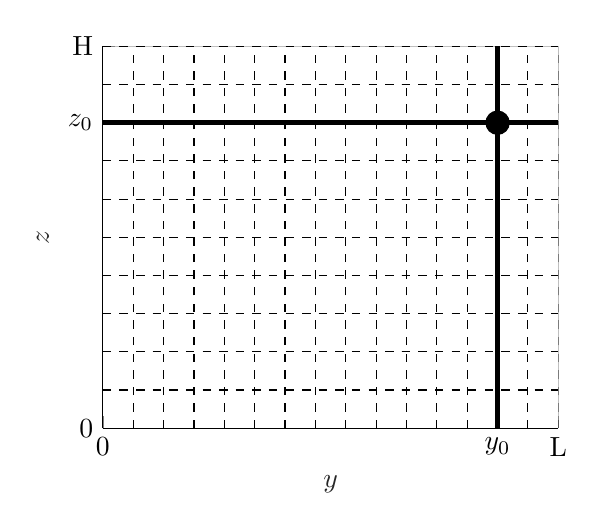
\begin{tikzpicture}

\begin{axis}[%
width=0.477\textwidth,
height=0.4\textwidth,
at={(0\textwidth,0\textwidth)},
scale only axis,
xmin=0,
xmax=15,
xtick={0,13,15},
xticklabels={{0},{$y_0$},{L}},
xlabel style={font=\color{white!15!black}},
xlabel={$y$},
ymin=0,
ymax=5,
ytick={0,4,5},
yticklabels={{0},{$z_0$},{H}},
ylabel style={font=\color{white!15!black}},
ylabel={$z$},
axis background/.style={fill=white},
axis x line*=bottom,
axis y line*=left,
xmajorgrids,
ymajorgrids
]
\addplot [color=black, dashed, forget plot]
  table[row sep=crcr]{%
0	0\\
0	0.0505050505050505\\
0	0.101010101010101\\
0	0.151515151515152\\
0	0.202020202020202\\
0	0.252525252525253\\
0	0.303030303030303\\
0	0.353535353535354\\
0	0.404040404040404\\
0	0.454545454545455\\
0	0.505050505050505\\
0	0.555555555555556\\
0	0.606060606060606\\
0	0.656565656565657\\
0	0.707070707070707\\
0	0.757575757575758\\
0	0.808080808080808\\
0	0.858585858585859\\
0	0.909090909090909\\
0	0.95959595959596\\
0	1.01010101010101\\
0	1.06060606060606\\
0	1.11111111111111\\
0	1.16161616161616\\
0	1.21212121212121\\
0	1.26262626262626\\
0	1.31313131313131\\
0	1.36363636363636\\
0	1.41414141414141\\
0	1.46464646464646\\
0	1.51515151515152\\
0	1.56565656565657\\
0	1.61616161616162\\
0	1.66666666666667\\
0	1.71717171717172\\
0	1.76767676767677\\
0	1.81818181818182\\
0	1.86868686868687\\
0	1.91919191919192\\
0	1.96969696969697\\
0	2.02020202020202\\
0	2.07070707070707\\
0	2.12121212121212\\
0	2.17171717171717\\
0	2.22222222222222\\
0	2.27272727272727\\
0	2.32323232323232\\
0	2.37373737373737\\
0	2.42424242424242\\
0	2.47474747474747\\
0	2.52525252525253\\
0	2.57575757575758\\
0	2.62626262626263\\
0	2.67676767676768\\
0	2.72727272727273\\
0	2.77777777777778\\
0	2.82828282828283\\
0	2.87878787878788\\
0	2.92929292929293\\
0	2.97979797979798\\
0	3.03030303030303\\
0	3.08080808080808\\
0	3.13131313131313\\
0	3.18181818181818\\
0	3.23232323232323\\
0	3.28282828282828\\
0	3.33333333333333\\
0	3.38383838383838\\
0	3.43434343434343\\
0	3.48484848484848\\
0	3.53535353535354\\
0	3.58585858585859\\
0	3.63636363636364\\
0	3.68686868686869\\
0	3.73737373737374\\
0	3.78787878787879\\
0	3.83838383838384\\
0	3.88888888888889\\
0	3.93939393939394\\
0	3.98989898989899\\
0	4.04040404040404\\
0	4.09090909090909\\
0	4.14141414141414\\
0	4.19191919191919\\
0	4.24242424242424\\
0	4.29292929292929\\
0	4.34343434343434\\
0	4.39393939393939\\
0	4.44444444444444\\
0	4.49494949494949\\
0	4.54545454545455\\
0	4.5959595959596\\
0	4.64646464646465\\
0	4.6969696969697\\
0	4.74747474747475\\
0	4.7979797979798\\
0	4.84848484848485\\
0	4.8989898989899\\
0	4.94949494949495\\
0	5\\
};
\addplot [color=black, dashed, forget plot]
  table[row sep=crcr]{%
1	0\\
1	0.0505050505050505\\
1	0.101010101010101\\
1	0.151515151515152\\
1	0.202020202020202\\
1	0.252525252525253\\
1	0.303030303030303\\
1	0.353535353535354\\
1	0.404040404040404\\
1	0.454545454545455\\
1	0.505050505050505\\
1	0.555555555555556\\
1	0.606060606060606\\
1	0.656565656565657\\
1	0.707070707070707\\
1	0.757575757575758\\
1	0.808080808080808\\
1	0.858585858585859\\
1	0.909090909090909\\
1	0.95959595959596\\
1	1.01010101010101\\
1	1.06060606060606\\
1	1.11111111111111\\
1	1.16161616161616\\
1	1.21212121212121\\
1	1.26262626262626\\
1	1.31313131313131\\
1	1.36363636363636\\
1	1.41414141414141\\
1	1.46464646464646\\
1	1.51515151515152\\
1	1.56565656565657\\
1	1.61616161616162\\
1	1.66666666666667\\
1	1.71717171717172\\
1	1.76767676767677\\
1	1.81818181818182\\
1	1.86868686868687\\
1	1.91919191919192\\
1	1.96969696969697\\
1	2.02020202020202\\
1	2.07070707070707\\
1	2.12121212121212\\
1	2.17171717171717\\
1	2.22222222222222\\
1	2.27272727272727\\
1	2.32323232323232\\
1	2.37373737373737\\
1	2.42424242424242\\
1	2.47474747474747\\
1	2.52525252525253\\
1	2.57575757575758\\
1	2.62626262626263\\
1	2.67676767676768\\
1	2.72727272727273\\
1	2.77777777777778\\
1	2.82828282828283\\
1	2.87878787878788\\
1	2.92929292929293\\
1	2.97979797979798\\
1	3.03030303030303\\
1	3.08080808080808\\
1	3.13131313131313\\
1	3.18181818181818\\
1	3.23232323232323\\
1	3.28282828282828\\
1	3.33333333333333\\
1	3.38383838383838\\
1	3.43434343434343\\
1	3.48484848484848\\
1	3.53535353535354\\
1	3.58585858585859\\
1	3.63636363636364\\
1	3.68686868686869\\
1	3.73737373737374\\
1	3.78787878787879\\
1	3.83838383838384\\
1	3.88888888888889\\
1	3.93939393939394\\
1	3.98989898989899\\
1	4.04040404040404\\
1	4.09090909090909\\
1	4.14141414141414\\
1	4.19191919191919\\
1	4.24242424242424\\
1	4.29292929292929\\
1	4.34343434343434\\
1	4.39393939393939\\
1	4.44444444444444\\
1	4.49494949494949\\
1	4.54545454545455\\
1	4.5959595959596\\
1	4.64646464646465\\
1	4.6969696969697\\
1	4.74747474747475\\
1	4.7979797979798\\
1	4.84848484848485\\
1	4.8989898989899\\
1	4.94949494949495\\
1	5\\
};
\addplot [color=black, dashed, forget plot]
  table[row sep=crcr]{%
2	0\\
2	0.0505050505050505\\
2	0.101010101010101\\
2	0.151515151515152\\
2	0.202020202020202\\
2	0.252525252525253\\
2	0.303030303030303\\
2	0.353535353535354\\
2	0.404040404040404\\
2	0.454545454545455\\
2	0.505050505050505\\
2	0.555555555555556\\
2	0.606060606060606\\
2	0.656565656565657\\
2	0.707070707070707\\
2	0.757575757575758\\
2	0.808080808080808\\
2	0.858585858585859\\
2	0.909090909090909\\
2	0.95959595959596\\
2	1.01010101010101\\
2	1.06060606060606\\
2	1.11111111111111\\
2	1.16161616161616\\
2	1.21212121212121\\
2	1.26262626262626\\
2	1.31313131313131\\
2	1.36363636363636\\
2	1.41414141414141\\
2	1.46464646464646\\
2	1.51515151515152\\
2	1.56565656565657\\
2	1.61616161616162\\
2	1.66666666666667\\
2	1.71717171717172\\
2	1.76767676767677\\
2	1.81818181818182\\
2	1.86868686868687\\
2	1.91919191919192\\
2	1.96969696969697\\
2	2.02020202020202\\
2	2.07070707070707\\
2	2.12121212121212\\
2	2.17171717171717\\
2	2.22222222222222\\
2	2.27272727272727\\
2	2.32323232323232\\
2	2.37373737373737\\
2	2.42424242424242\\
2	2.47474747474747\\
2	2.52525252525253\\
2	2.57575757575758\\
2	2.62626262626263\\
2	2.67676767676768\\
2	2.72727272727273\\
2	2.77777777777778\\
2	2.82828282828283\\
2	2.87878787878788\\
2	2.92929292929293\\
2	2.97979797979798\\
2	3.03030303030303\\
2	3.08080808080808\\
2	3.13131313131313\\
2	3.18181818181818\\
2	3.23232323232323\\
2	3.28282828282828\\
2	3.33333333333333\\
2	3.38383838383838\\
2	3.43434343434343\\
2	3.48484848484848\\
2	3.53535353535354\\
2	3.58585858585859\\
2	3.63636363636364\\
2	3.68686868686869\\
2	3.73737373737374\\
2	3.78787878787879\\
2	3.83838383838384\\
2	3.88888888888889\\
2	3.93939393939394\\
2	3.98989898989899\\
2	4.04040404040404\\
2	4.09090909090909\\
2	4.14141414141414\\
2	4.19191919191919\\
2	4.24242424242424\\
2	4.29292929292929\\
2	4.34343434343434\\
2	4.39393939393939\\
2	4.44444444444444\\
2	4.49494949494949\\
2	4.54545454545455\\
2	4.5959595959596\\
2	4.64646464646465\\
2	4.6969696969697\\
2	4.74747474747475\\
2	4.7979797979798\\
2	4.84848484848485\\
2	4.8989898989899\\
2	4.94949494949495\\
2	5\\
};
\addplot [color=black, dashed, forget plot]
  table[row sep=crcr]{%
3	0\\
3	0.0505050505050505\\
3	0.101010101010101\\
3	0.151515151515152\\
3	0.202020202020202\\
3	0.252525252525253\\
3	0.303030303030303\\
3	0.353535353535354\\
3	0.404040404040404\\
3	0.454545454545455\\
3	0.505050505050505\\
3	0.555555555555556\\
3	0.606060606060606\\
3	0.656565656565657\\
3	0.707070707070707\\
3	0.757575757575758\\
3	0.808080808080808\\
3	0.858585858585859\\
3	0.909090909090909\\
3	0.95959595959596\\
3	1.01010101010101\\
3	1.06060606060606\\
3	1.11111111111111\\
3	1.16161616161616\\
3	1.21212121212121\\
3	1.26262626262626\\
3	1.31313131313131\\
3	1.36363636363636\\
3	1.41414141414141\\
3	1.46464646464646\\
3	1.51515151515152\\
3	1.56565656565657\\
3	1.61616161616162\\
3	1.66666666666667\\
3	1.71717171717172\\
3	1.76767676767677\\
3	1.81818181818182\\
3	1.86868686868687\\
3	1.91919191919192\\
3	1.96969696969697\\
3	2.02020202020202\\
3	2.07070707070707\\
3	2.12121212121212\\
3	2.17171717171717\\
3	2.22222222222222\\
3	2.27272727272727\\
3	2.32323232323232\\
3	2.37373737373737\\
3	2.42424242424242\\
3	2.47474747474747\\
3	2.52525252525253\\
3	2.57575757575758\\
3	2.62626262626263\\
3	2.67676767676768\\
3	2.72727272727273\\
3	2.77777777777778\\
3	2.82828282828283\\
3	2.87878787878788\\
3	2.92929292929293\\
3	2.97979797979798\\
3	3.03030303030303\\
3	3.08080808080808\\
3	3.13131313131313\\
3	3.18181818181818\\
3	3.23232323232323\\
3	3.28282828282828\\
3	3.33333333333333\\
3	3.38383838383838\\
3	3.43434343434343\\
3	3.48484848484848\\
3	3.53535353535354\\
3	3.58585858585859\\
3	3.63636363636364\\
3	3.68686868686869\\
3	3.73737373737374\\
3	3.78787878787879\\
3	3.83838383838384\\
3	3.88888888888889\\
3	3.93939393939394\\
3	3.98989898989899\\
3	4.04040404040404\\
3	4.09090909090909\\
3	4.14141414141414\\
3	4.19191919191919\\
3	4.24242424242424\\
3	4.29292929292929\\
3	4.34343434343434\\
3	4.39393939393939\\
3	4.44444444444444\\
3	4.49494949494949\\
3	4.54545454545455\\
3	4.5959595959596\\
3	4.64646464646465\\
3	4.6969696969697\\
3	4.74747474747475\\
3	4.7979797979798\\
3	4.84848484848485\\
3	4.8989898989899\\
3	4.94949494949495\\
3	5\\
};
\addplot [color=black, dashed, forget plot]
  table[row sep=crcr]{%
4	0\\
4	0.0505050505050505\\
4	0.101010101010101\\
4	0.151515151515152\\
4	0.202020202020202\\
4	0.252525252525253\\
4	0.303030303030303\\
4	0.353535353535354\\
4	0.404040404040404\\
4	0.454545454545455\\
4	0.505050505050505\\
4	0.555555555555556\\
4	0.606060606060606\\
4	0.656565656565657\\
4	0.707070707070707\\
4	0.757575757575758\\
4	0.808080808080808\\
4	0.858585858585859\\
4	0.909090909090909\\
4	0.95959595959596\\
4	1.01010101010101\\
4	1.06060606060606\\
4	1.11111111111111\\
4	1.16161616161616\\
4	1.21212121212121\\
4	1.26262626262626\\
4	1.31313131313131\\
4	1.36363636363636\\
4	1.41414141414141\\
4	1.46464646464646\\
4	1.51515151515152\\
4	1.56565656565657\\
4	1.61616161616162\\
4	1.66666666666667\\
4	1.71717171717172\\
4	1.76767676767677\\
4	1.81818181818182\\
4	1.86868686868687\\
4	1.91919191919192\\
4	1.96969696969697\\
4	2.02020202020202\\
4	2.07070707070707\\
4	2.12121212121212\\
4	2.17171717171717\\
4	2.22222222222222\\
4	2.27272727272727\\
4	2.32323232323232\\
4	2.37373737373737\\
4	2.42424242424242\\
4	2.47474747474747\\
4	2.52525252525253\\
4	2.57575757575758\\
4	2.62626262626263\\
4	2.67676767676768\\
4	2.72727272727273\\
4	2.77777777777778\\
4	2.82828282828283\\
4	2.87878787878788\\
4	2.92929292929293\\
4	2.97979797979798\\
4	3.03030303030303\\
4	3.08080808080808\\
4	3.13131313131313\\
4	3.18181818181818\\
4	3.23232323232323\\
4	3.28282828282828\\
4	3.33333333333333\\
4	3.38383838383838\\
4	3.43434343434343\\
4	3.48484848484848\\
4	3.53535353535354\\
4	3.58585858585859\\
4	3.63636363636364\\
4	3.68686868686869\\
4	3.73737373737374\\
4	3.78787878787879\\
4	3.83838383838384\\
4	3.88888888888889\\
4	3.93939393939394\\
4	3.98989898989899\\
4	4.04040404040404\\
4	4.09090909090909\\
4	4.14141414141414\\
4	4.19191919191919\\
4	4.24242424242424\\
4	4.29292929292929\\
4	4.34343434343434\\
4	4.39393939393939\\
4	4.44444444444444\\
4	4.49494949494949\\
4	4.54545454545455\\
4	4.5959595959596\\
4	4.64646464646465\\
4	4.6969696969697\\
4	4.74747474747475\\
4	4.7979797979798\\
4	4.84848484848485\\
4	4.8989898989899\\
4	4.94949494949495\\
4	5\\
};
\addplot [color=black, dashed, forget plot]
  table[row sep=crcr]{%
5	0\\
5	0.0505050505050505\\
5	0.101010101010101\\
5	0.151515151515152\\
5	0.202020202020202\\
5	0.252525252525253\\
5	0.303030303030303\\
5	0.353535353535354\\
5	0.404040404040404\\
5	0.454545454545455\\
5	0.505050505050505\\
5	0.555555555555556\\
5	0.606060606060606\\
5	0.656565656565657\\
5	0.707070707070707\\
5	0.757575757575758\\
5	0.808080808080808\\
5	0.858585858585859\\
5	0.909090909090909\\
5	0.95959595959596\\
5	1.01010101010101\\
5	1.06060606060606\\
5	1.11111111111111\\
5	1.16161616161616\\
5	1.21212121212121\\
5	1.26262626262626\\
5	1.31313131313131\\
5	1.36363636363636\\
5	1.41414141414141\\
5	1.46464646464646\\
5	1.51515151515152\\
5	1.56565656565657\\
5	1.61616161616162\\
5	1.66666666666667\\
5	1.71717171717172\\
5	1.76767676767677\\
5	1.81818181818182\\
5	1.86868686868687\\
5	1.91919191919192\\
5	1.96969696969697\\
5	2.02020202020202\\
5	2.07070707070707\\
5	2.12121212121212\\
5	2.17171717171717\\
5	2.22222222222222\\
5	2.27272727272727\\
5	2.32323232323232\\
5	2.37373737373737\\
5	2.42424242424242\\
5	2.47474747474747\\
5	2.52525252525253\\
5	2.57575757575758\\
5	2.62626262626263\\
5	2.67676767676768\\
5	2.72727272727273\\
5	2.77777777777778\\
5	2.82828282828283\\
5	2.87878787878788\\
5	2.92929292929293\\
5	2.97979797979798\\
5	3.03030303030303\\
5	3.08080808080808\\
5	3.13131313131313\\
5	3.18181818181818\\
5	3.23232323232323\\
5	3.28282828282828\\
5	3.33333333333333\\
5	3.38383838383838\\
5	3.43434343434343\\
5	3.48484848484848\\
5	3.53535353535354\\
5	3.58585858585859\\
5	3.63636363636364\\
5	3.68686868686869\\
5	3.73737373737374\\
5	3.78787878787879\\
5	3.83838383838384\\
5	3.88888888888889\\
5	3.93939393939394\\
5	3.98989898989899\\
5	4.04040404040404\\
5	4.09090909090909\\
5	4.14141414141414\\
5	4.19191919191919\\
5	4.24242424242424\\
5	4.29292929292929\\
5	4.34343434343434\\
5	4.39393939393939\\
5	4.44444444444444\\
5	4.49494949494949\\
5	4.54545454545455\\
5	4.5959595959596\\
5	4.64646464646465\\
5	4.6969696969697\\
5	4.74747474747475\\
5	4.7979797979798\\
5	4.84848484848485\\
5	4.8989898989899\\
5	4.94949494949495\\
5	5\\
};
\addplot [color=black, dashed, forget plot]
  table[row sep=crcr]{%
6	0\\
6	0.0505050505050505\\
6	0.101010101010101\\
6	0.151515151515152\\
6	0.202020202020202\\
6	0.252525252525253\\
6	0.303030303030303\\
6	0.353535353535354\\
6	0.404040404040404\\
6	0.454545454545455\\
6	0.505050505050505\\
6	0.555555555555556\\
6	0.606060606060606\\
6	0.656565656565657\\
6	0.707070707070707\\
6	0.757575757575758\\
6	0.808080808080808\\
6	0.858585858585859\\
6	0.909090909090909\\
6	0.95959595959596\\
6	1.01010101010101\\
6	1.06060606060606\\
6	1.11111111111111\\
6	1.16161616161616\\
6	1.21212121212121\\
6	1.26262626262626\\
6	1.31313131313131\\
6	1.36363636363636\\
6	1.41414141414141\\
6	1.46464646464646\\
6	1.51515151515152\\
6	1.56565656565657\\
6	1.61616161616162\\
6	1.66666666666667\\
6	1.71717171717172\\
6	1.76767676767677\\
6	1.81818181818182\\
6	1.86868686868687\\
6	1.91919191919192\\
6	1.96969696969697\\
6	2.02020202020202\\
6	2.07070707070707\\
6	2.12121212121212\\
6	2.17171717171717\\
6	2.22222222222222\\
6	2.27272727272727\\
6	2.32323232323232\\
6	2.37373737373737\\
6	2.42424242424242\\
6	2.47474747474747\\
6	2.52525252525253\\
6	2.57575757575758\\
6	2.62626262626263\\
6	2.67676767676768\\
6	2.72727272727273\\
6	2.77777777777778\\
6	2.82828282828283\\
6	2.87878787878788\\
6	2.92929292929293\\
6	2.97979797979798\\
6	3.03030303030303\\
6	3.08080808080808\\
6	3.13131313131313\\
6	3.18181818181818\\
6	3.23232323232323\\
6	3.28282828282828\\
6	3.33333333333333\\
6	3.38383838383838\\
6	3.43434343434343\\
6	3.48484848484848\\
6	3.53535353535354\\
6	3.58585858585859\\
6	3.63636363636364\\
6	3.68686868686869\\
6	3.73737373737374\\
6	3.78787878787879\\
6	3.83838383838384\\
6	3.88888888888889\\
6	3.93939393939394\\
6	3.98989898989899\\
6	4.04040404040404\\
6	4.09090909090909\\
6	4.14141414141414\\
6	4.19191919191919\\
6	4.24242424242424\\
6	4.29292929292929\\
6	4.34343434343434\\
6	4.39393939393939\\
6	4.44444444444444\\
6	4.49494949494949\\
6	4.54545454545455\\
6	4.5959595959596\\
6	4.64646464646465\\
6	4.6969696969697\\
6	4.74747474747475\\
6	4.7979797979798\\
6	4.84848484848485\\
6	4.8989898989899\\
6	4.94949494949495\\
6	5\\
};
\addplot [color=black, dashed, forget plot]
  table[row sep=crcr]{%
7	0\\
7	0.0505050505050505\\
7	0.101010101010101\\
7	0.151515151515152\\
7	0.202020202020202\\
7	0.252525252525253\\
7	0.303030303030303\\
7	0.353535353535354\\
7	0.404040404040404\\
7	0.454545454545455\\
7	0.505050505050505\\
7	0.555555555555556\\
7	0.606060606060606\\
7	0.656565656565657\\
7	0.707070707070707\\
7	0.757575757575758\\
7	0.808080808080808\\
7	0.858585858585859\\
7	0.909090909090909\\
7	0.95959595959596\\
7	1.01010101010101\\
7	1.06060606060606\\
7	1.11111111111111\\
7	1.16161616161616\\
7	1.21212121212121\\
7	1.26262626262626\\
7	1.31313131313131\\
7	1.36363636363636\\
7	1.41414141414141\\
7	1.46464646464646\\
7	1.51515151515152\\
7	1.56565656565657\\
7	1.61616161616162\\
7	1.66666666666667\\
7	1.71717171717172\\
7	1.76767676767677\\
7	1.81818181818182\\
7	1.86868686868687\\
7	1.91919191919192\\
7	1.96969696969697\\
7	2.02020202020202\\
7	2.07070707070707\\
7	2.12121212121212\\
7	2.17171717171717\\
7	2.22222222222222\\
7	2.27272727272727\\
7	2.32323232323232\\
7	2.37373737373737\\
7	2.42424242424242\\
7	2.47474747474747\\
7	2.52525252525253\\
7	2.57575757575758\\
7	2.62626262626263\\
7	2.67676767676768\\
7	2.72727272727273\\
7	2.77777777777778\\
7	2.82828282828283\\
7	2.87878787878788\\
7	2.92929292929293\\
7	2.97979797979798\\
7	3.03030303030303\\
7	3.08080808080808\\
7	3.13131313131313\\
7	3.18181818181818\\
7	3.23232323232323\\
7	3.28282828282828\\
7	3.33333333333333\\
7	3.38383838383838\\
7	3.43434343434343\\
7	3.48484848484848\\
7	3.53535353535354\\
7	3.58585858585859\\
7	3.63636363636364\\
7	3.68686868686869\\
7	3.73737373737374\\
7	3.78787878787879\\
7	3.83838383838384\\
7	3.88888888888889\\
7	3.93939393939394\\
7	3.98989898989899\\
7	4.04040404040404\\
7	4.09090909090909\\
7	4.14141414141414\\
7	4.19191919191919\\
7	4.24242424242424\\
7	4.29292929292929\\
7	4.34343434343434\\
7	4.39393939393939\\
7	4.44444444444444\\
7	4.49494949494949\\
7	4.54545454545455\\
7	4.5959595959596\\
7	4.64646464646465\\
7	4.6969696969697\\
7	4.74747474747475\\
7	4.7979797979798\\
7	4.84848484848485\\
7	4.8989898989899\\
7	4.94949494949495\\
7	5\\
};
\addplot [color=black, dashed, forget plot]
  table[row sep=crcr]{%
8	0\\
8	0.0505050505050505\\
8	0.101010101010101\\
8	0.151515151515152\\
8	0.202020202020202\\
8	0.252525252525253\\
8	0.303030303030303\\
8	0.353535353535354\\
8	0.404040404040404\\
8	0.454545454545455\\
8	0.505050505050505\\
8	0.555555555555556\\
8	0.606060606060606\\
8	0.656565656565657\\
8	0.707070707070707\\
8	0.757575757575758\\
8	0.808080808080808\\
8	0.858585858585859\\
8	0.909090909090909\\
8	0.95959595959596\\
8	1.01010101010101\\
8	1.06060606060606\\
8	1.11111111111111\\
8	1.16161616161616\\
8	1.21212121212121\\
8	1.26262626262626\\
8	1.31313131313131\\
8	1.36363636363636\\
8	1.41414141414141\\
8	1.46464646464646\\
8	1.51515151515152\\
8	1.56565656565657\\
8	1.61616161616162\\
8	1.66666666666667\\
8	1.71717171717172\\
8	1.76767676767677\\
8	1.81818181818182\\
8	1.86868686868687\\
8	1.91919191919192\\
8	1.96969696969697\\
8	2.02020202020202\\
8	2.07070707070707\\
8	2.12121212121212\\
8	2.17171717171717\\
8	2.22222222222222\\
8	2.27272727272727\\
8	2.32323232323232\\
8	2.37373737373737\\
8	2.42424242424242\\
8	2.47474747474747\\
8	2.52525252525253\\
8	2.57575757575758\\
8	2.62626262626263\\
8	2.67676767676768\\
8	2.72727272727273\\
8	2.77777777777778\\
8	2.82828282828283\\
8	2.87878787878788\\
8	2.92929292929293\\
8	2.97979797979798\\
8	3.03030303030303\\
8	3.08080808080808\\
8	3.13131313131313\\
8	3.18181818181818\\
8	3.23232323232323\\
8	3.28282828282828\\
8	3.33333333333333\\
8	3.38383838383838\\
8	3.43434343434343\\
8	3.48484848484848\\
8	3.53535353535354\\
8	3.58585858585859\\
8	3.63636363636364\\
8	3.68686868686869\\
8	3.73737373737374\\
8	3.78787878787879\\
8	3.83838383838384\\
8	3.88888888888889\\
8	3.93939393939394\\
8	3.98989898989899\\
8	4.04040404040404\\
8	4.09090909090909\\
8	4.14141414141414\\
8	4.19191919191919\\
8	4.24242424242424\\
8	4.29292929292929\\
8	4.34343434343434\\
8	4.39393939393939\\
8	4.44444444444444\\
8	4.49494949494949\\
8	4.54545454545455\\
8	4.5959595959596\\
8	4.64646464646465\\
8	4.6969696969697\\
8	4.74747474747475\\
8	4.7979797979798\\
8	4.84848484848485\\
8	4.8989898989899\\
8	4.94949494949495\\
8	5\\
};
\addplot [color=black, dashed, forget plot]
  table[row sep=crcr]{%
9	0\\
9	0.0505050505050505\\
9	0.101010101010101\\
9	0.151515151515152\\
9	0.202020202020202\\
9	0.252525252525253\\
9	0.303030303030303\\
9	0.353535353535354\\
9	0.404040404040404\\
9	0.454545454545455\\
9	0.505050505050505\\
9	0.555555555555556\\
9	0.606060606060606\\
9	0.656565656565657\\
9	0.707070707070707\\
9	0.757575757575758\\
9	0.808080808080808\\
9	0.858585858585859\\
9	0.909090909090909\\
9	0.95959595959596\\
9	1.01010101010101\\
9	1.06060606060606\\
9	1.11111111111111\\
9	1.16161616161616\\
9	1.21212121212121\\
9	1.26262626262626\\
9	1.31313131313131\\
9	1.36363636363636\\
9	1.41414141414141\\
9	1.46464646464646\\
9	1.51515151515152\\
9	1.56565656565657\\
9	1.61616161616162\\
9	1.66666666666667\\
9	1.71717171717172\\
9	1.76767676767677\\
9	1.81818181818182\\
9	1.86868686868687\\
9	1.91919191919192\\
9	1.96969696969697\\
9	2.02020202020202\\
9	2.07070707070707\\
9	2.12121212121212\\
9	2.17171717171717\\
9	2.22222222222222\\
9	2.27272727272727\\
9	2.32323232323232\\
9	2.37373737373737\\
9	2.42424242424242\\
9	2.47474747474747\\
9	2.52525252525253\\
9	2.57575757575758\\
9	2.62626262626263\\
9	2.67676767676768\\
9	2.72727272727273\\
9	2.77777777777778\\
9	2.82828282828283\\
9	2.87878787878788\\
9	2.92929292929293\\
9	2.97979797979798\\
9	3.03030303030303\\
9	3.08080808080808\\
9	3.13131313131313\\
9	3.18181818181818\\
9	3.23232323232323\\
9	3.28282828282828\\
9	3.33333333333333\\
9	3.38383838383838\\
9	3.43434343434343\\
9	3.48484848484848\\
9	3.53535353535354\\
9	3.58585858585859\\
9	3.63636363636364\\
9	3.68686868686869\\
9	3.73737373737374\\
9	3.78787878787879\\
9	3.83838383838384\\
9	3.88888888888889\\
9	3.93939393939394\\
9	3.98989898989899\\
9	4.04040404040404\\
9	4.09090909090909\\
9	4.14141414141414\\
9	4.19191919191919\\
9	4.24242424242424\\
9	4.29292929292929\\
9	4.34343434343434\\
9	4.39393939393939\\
9	4.44444444444444\\
9	4.49494949494949\\
9	4.54545454545455\\
9	4.5959595959596\\
9	4.64646464646465\\
9	4.6969696969697\\
9	4.74747474747475\\
9	4.7979797979798\\
9	4.84848484848485\\
9	4.8989898989899\\
9	4.94949494949495\\
9	5\\
};
\addplot [color=black, dashed, forget plot]
  table[row sep=crcr]{%
10	0\\
10	0.0505050505050505\\
10	0.101010101010101\\
10	0.151515151515152\\
10	0.202020202020202\\
10	0.252525252525253\\
10	0.303030303030303\\
10	0.353535353535354\\
10	0.404040404040404\\
10	0.454545454545455\\
10	0.505050505050505\\
10	0.555555555555556\\
10	0.606060606060606\\
10	0.656565656565657\\
10	0.707070707070707\\
10	0.757575757575758\\
10	0.808080808080808\\
10	0.858585858585859\\
10	0.909090909090909\\
10	0.95959595959596\\
10	1.01010101010101\\
10	1.06060606060606\\
10	1.11111111111111\\
10	1.16161616161616\\
10	1.21212121212121\\
10	1.26262626262626\\
10	1.31313131313131\\
10	1.36363636363636\\
10	1.41414141414141\\
10	1.46464646464646\\
10	1.51515151515152\\
10	1.56565656565657\\
10	1.61616161616162\\
10	1.66666666666667\\
10	1.71717171717172\\
10	1.76767676767677\\
10	1.81818181818182\\
10	1.86868686868687\\
10	1.91919191919192\\
10	1.96969696969697\\
10	2.02020202020202\\
10	2.07070707070707\\
10	2.12121212121212\\
10	2.17171717171717\\
10	2.22222222222222\\
10	2.27272727272727\\
10	2.32323232323232\\
10	2.37373737373737\\
10	2.42424242424242\\
10	2.47474747474747\\
10	2.52525252525253\\
10	2.57575757575758\\
10	2.62626262626263\\
10	2.67676767676768\\
10	2.72727272727273\\
10	2.77777777777778\\
10	2.82828282828283\\
10	2.87878787878788\\
10	2.92929292929293\\
10	2.97979797979798\\
10	3.03030303030303\\
10	3.08080808080808\\
10	3.13131313131313\\
10	3.18181818181818\\
10	3.23232323232323\\
10	3.28282828282828\\
10	3.33333333333333\\
10	3.38383838383838\\
10	3.43434343434343\\
10	3.48484848484848\\
10	3.53535353535354\\
10	3.58585858585859\\
10	3.63636363636364\\
10	3.68686868686869\\
10	3.73737373737374\\
10	3.78787878787879\\
10	3.83838383838384\\
10	3.88888888888889\\
10	3.93939393939394\\
10	3.98989898989899\\
10	4.04040404040404\\
10	4.09090909090909\\
10	4.14141414141414\\
10	4.19191919191919\\
10	4.24242424242424\\
10	4.29292929292929\\
10	4.34343434343434\\
10	4.39393939393939\\
10	4.44444444444444\\
10	4.49494949494949\\
10	4.54545454545455\\
10	4.5959595959596\\
10	4.64646464646465\\
10	4.6969696969697\\
10	4.74747474747475\\
10	4.7979797979798\\
10	4.84848484848485\\
10	4.8989898989899\\
10	4.94949494949495\\
10	5\\
};
\addplot [color=black, dashed, forget plot]
  table[row sep=crcr]{%
11	0\\
11	0.0505050505050505\\
11	0.101010101010101\\
11	0.151515151515152\\
11	0.202020202020202\\
11	0.252525252525253\\
11	0.303030303030303\\
11	0.353535353535354\\
11	0.404040404040404\\
11	0.454545454545455\\
11	0.505050505050505\\
11	0.555555555555556\\
11	0.606060606060606\\
11	0.656565656565657\\
11	0.707070707070707\\
11	0.757575757575758\\
11	0.808080808080808\\
11	0.858585858585859\\
11	0.909090909090909\\
11	0.95959595959596\\
11	1.01010101010101\\
11	1.06060606060606\\
11	1.11111111111111\\
11	1.16161616161616\\
11	1.21212121212121\\
11	1.26262626262626\\
11	1.31313131313131\\
11	1.36363636363636\\
11	1.41414141414141\\
11	1.46464646464646\\
11	1.51515151515152\\
11	1.56565656565657\\
11	1.61616161616162\\
11	1.66666666666667\\
11	1.71717171717172\\
11	1.76767676767677\\
11	1.81818181818182\\
11	1.86868686868687\\
11	1.91919191919192\\
11	1.96969696969697\\
11	2.02020202020202\\
11	2.07070707070707\\
11	2.12121212121212\\
11	2.17171717171717\\
11	2.22222222222222\\
11	2.27272727272727\\
11	2.32323232323232\\
11	2.37373737373737\\
11	2.42424242424242\\
11	2.47474747474747\\
11	2.52525252525253\\
11	2.57575757575758\\
11	2.62626262626263\\
11	2.67676767676768\\
11	2.72727272727273\\
11	2.77777777777778\\
11	2.82828282828283\\
11	2.87878787878788\\
11	2.92929292929293\\
11	2.97979797979798\\
11	3.03030303030303\\
11	3.08080808080808\\
11	3.13131313131313\\
11	3.18181818181818\\
11	3.23232323232323\\
11	3.28282828282828\\
11	3.33333333333333\\
11	3.38383838383838\\
11	3.43434343434343\\
11	3.48484848484848\\
11	3.53535353535354\\
11	3.58585858585859\\
11	3.63636363636364\\
11	3.68686868686869\\
11	3.73737373737374\\
11	3.78787878787879\\
11	3.83838383838384\\
11	3.88888888888889\\
11	3.93939393939394\\
11	3.98989898989899\\
11	4.04040404040404\\
11	4.09090909090909\\
11	4.14141414141414\\
11	4.19191919191919\\
11	4.24242424242424\\
11	4.29292929292929\\
11	4.34343434343434\\
11	4.39393939393939\\
11	4.44444444444444\\
11	4.49494949494949\\
11	4.54545454545455\\
11	4.5959595959596\\
11	4.64646464646465\\
11	4.6969696969697\\
11	4.74747474747475\\
11	4.7979797979798\\
11	4.84848484848485\\
11	4.8989898989899\\
11	4.94949494949495\\
11	5\\
};
\addplot [color=black, dashed, forget plot]
  table[row sep=crcr]{%
12	0\\
12	0.0505050505050505\\
12	0.101010101010101\\
12	0.151515151515152\\
12	0.202020202020202\\
12	0.252525252525253\\
12	0.303030303030303\\
12	0.353535353535354\\
12	0.404040404040404\\
12	0.454545454545455\\
12	0.505050505050505\\
12	0.555555555555556\\
12	0.606060606060606\\
12	0.656565656565657\\
12	0.707070707070707\\
12	0.757575757575758\\
12	0.808080808080808\\
12	0.858585858585859\\
12	0.909090909090909\\
12	0.95959595959596\\
12	1.01010101010101\\
12	1.06060606060606\\
12	1.11111111111111\\
12	1.16161616161616\\
12	1.21212121212121\\
12	1.26262626262626\\
12	1.31313131313131\\
12	1.36363636363636\\
12	1.41414141414141\\
12	1.46464646464646\\
12	1.51515151515152\\
12	1.56565656565657\\
12	1.61616161616162\\
12	1.66666666666667\\
12	1.71717171717172\\
12	1.76767676767677\\
12	1.81818181818182\\
12	1.86868686868687\\
12	1.91919191919192\\
12	1.96969696969697\\
12	2.02020202020202\\
12	2.07070707070707\\
12	2.12121212121212\\
12	2.17171717171717\\
12	2.22222222222222\\
12	2.27272727272727\\
12	2.32323232323232\\
12	2.37373737373737\\
12	2.42424242424242\\
12	2.47474747474747\\
12	2.52525252525253\\
12	2.57575757575758\\
12	2.62626262626263\\
12	2.67676767676768\\
12	2.72727272727273\\
12	2.77777777777778\\
12	2.82828282828283\\
12	2.87878787878788\\
12	2.92929292929293\\
12	2.97979797979798\\
12	3.03030303030303\\
12	3.08080808080808\\
12	3.13131313131313\\
12	3.18181818181818\\
12	3.23232323232323\\
12	3.28282828282828\\
12	3.33333333333333\\
12	3.38383838383838\\
12	3.43434343434343\\
12	3.48484848484848\\
12	3.53535353535354\\
12	3.58585858585859\\
12	3.63636363636364\\
12	3.68686868686869\\
12	3.73737373737374\\
12	3.78787878787879\\
12	3.83838383838384\\
12	3.88888888888889\\
12	3.93939393939394\\
12	3.98989898989899\\
12	4.04040404040404\\
12	4.09090909090909\\
12	4.14141414141414\\
12	4.19191919191919\\
12	4.24242424242424\\
12	4.29292929292929\\
12	4.34343434343434\\
12	4.39393939393939\\
12	4.44444444444444\\
12	4.49494949494949\\
12	4.54545454545455\\
12	4.5959595959596\\
12	4.64646464646465\\
12	4.6969696969697\\
12	4.74747474747475\\
12	4.7979797979798\\
12	4.84848484848485\\
12	4.8989898989899\\
12	4.94949494949495\\
12	5\\
};
\addplot [color=black, dashed, forget plot]
  table[row sep=crcr]{%
13	0\\
13	0.0505050505050505\\
13	0.101010101010101\\
13	0.151515151515152\\
13	0.202020202020202\\
13	0.252525252525253\\
13	0.303030303030303\\
13	0.353535353535354\\
13	0.404040404040404\\
13	0.454545454545455\\
13	0.505050505050505\\
13	0.555555555555556\\
13	0.606060606060606\\
13	0.656565656565657\\
13	0.707070707070707\\
13	0.757575757575758\\
13	0.808080808080808\\
13	0.858585858585859\\
13	0.909090909090909\\
13	0.95959595959596\\
13	1.01010101010101\\
13	1.06060606060606\\
13	1.11111111111111\\
13	1.16161616161616\\
13	1.21212121212121\\
13	1.26262626262626\\
13	1.31313131313131\\
13	1.36363636363636\\
13	1.41414141414141\\
13	1.46464646464646\\
13	1.51515151515152\\
13	1.56565656565657\\
13	1.61616161616162\\
13	1.66666666666667\\
13	1.71717171717172\\
13	1.76767676767677\\
13	1.81818181818182\\
13	1.86868686868687\\
13	1.91919191919192\\
13	1.96969696969697\\
13	2.02020202020202\\
13	2.07070707070707\\
13	2.12121212121212\\
13	2.17171717171717\\
13	2.22222222222222\\
13	2.27272727272727\\
13	2.32323232323232\\
13	2.37373737373737\\
13	2.42424242424242\\
13	2.47474747474747\\
13	2.52525252525253\\
13	2.57575757575758\\
13	2.62626262626263\\
13	2.67676767676768\\
13	2.72727272727273\\
13	2.77777777777778\\
13	2.82828282828283\\
13	2.87878787878788\\
13	2.92929292929293\\
13	2.97979797979798\\
13	3.03030303030303\\
13	3.08080808080808\\
13	3.13131313131313\\
13	3.18181818181818\\
13	3.23232323232323\\
13	3.28282828282828\\
13	3.33333333333333\\
13	3.38383838383838\\
13	3.43434343434343\\
13	3.48484848484848\\
13	3.53535353535354\\
13	3.58585858585859\\
13	3.63636363636364\\
13	3.68686868686869\\
13	3.73737373737374\\
13	3.78787878787879\\
13	3.83838383838384\\
13	3.88888888888889\\
13	3.93939393939394\\
13	3.98989898989899\\
13	4.04040404040404\\
13	4.09090909090909\\
13	4.14141414141414\\
13	4.19191919191919\\
13	4.24242424242424\\
13	4.29292929292929\\
13	4.34343434343434\\
13	4.39393939393939\\
13	4.44444444444444\\
13	4.49494949494949\\
13	4.54545454545455\\
13	4.5959595959596\\
13	4.64646464646465\\
13	4.6969696969697\\
13	4.74747474747475\\
13	4.7979797979798\\
13	4.84848484848485\\
13	4.8989898989899\\
13	4.94949494949495\\
13	5\\
};
\addplot [color=black, dashed, forget plot]
  table[row sep=crcr]{%
14	0\\
14	0.0505050505050505\\
14	0.101010101010101\\
14	0.151515151515152\\
14	0.202020202020202\\
14	0.252525252525253\\
14	0.303030303030303\\
14	0.353535353535354\\
14	0.404040404040404\\
14	0.454545454545455\\
14	0.505050505050505\\
14	0.555555555555556\\
14	0.606060606060606\\
14	0.656565656565657\\
14	0.707070707070707\\
14	0.757575757575758\\
14	0.808080808080808\\
14	0.858585858585859\\
14	0.909090909090909\\
14	0.95959595959596\\
14	1.01010101010101\\
14	1.06060606060606\\
14	1.11111111111111\\
14	1.16161616161616\\
14	1.21212121212121\\
14	1.26262626262626\\
14	1.31313131313131\\
14	1.36363636363636\\
14	1.41414141414141\\
14	1.46464646464646\\
14	1.51515151515152\\
14	1.56565656565657\\
14	1.61616161616162\\
14	1.66666666666667\\
14	1.71717171717172\\
14	1.76767676767677\\
14	1.81818181818182\\
14	1.86868686868687\\
14	1.91919191919192\\
14	1.96969696969697\\
14	2.02020202020202\\
14	2.07070707070707\\
14	2.12121212121212\\
14	2.17171717171717\\
14	2.22222222222222\\
14	2.27272727272727\\
14	2.32323232323232\\
14	2.37373737373737\\
14	2.42424242424242\\
14	2.47474747474747\\
14	2.52525252525253\\
14	2.57575757575758\\
14	2.62626262626263\\
14	2.67676767676768\\
14	2.72727272727273\\
14	2.77777777777778\\
14	2.82828282828283\\
14	2.87878787878788\\
14	2.92929292929293\\
14	2.97979797979798\\
14	3.03030303030303\\
14	3.08080808080808\\
14	3.13131313131313\\
14	3.18181818181818\\
14	3.23232323232323\\
14	3.28282828282828\\
14	3.33333333333333\\
14	3.38383838383838\\
14	3.43434343434343\\
14	3.48484848484848\\
14	3.53535353535354\\
14	3.58585858585859\\
14	3.63636363636364\\
14	3.68686868686869\\
14	3.73737373737374\\
14	3.78787878787879\\
14	3.83838383838384\\
14	3.88888888888889\\
14	3.93939393939394\\
14	3.98989898989899\\
14	4.04040404040404\\
14	4.09090909090909\\
14	4.14141414141414\\
14	4.19191919191919\\
14	4.24242424242424\\
14	4.29292929292929\\
14	4.34343434343434\\
14	4.39393939393939\\
14	4.44444444444444\\
14	4.49494949494949\\
14	4.54545454545455\\
14	4.5959595959596\\
14	4.64646464646465\\
14	4.6969696969697\\
14	4.74747474747475\\
14	4.7979797979798\\
14	4.84848484848485\\
14	4.8989898989899\\
14	4.94949494949495\\
14	5\\
};
\addplot [color=black, dashed, forget plot]
  table[row sep=crcr]{%
15	0\\
15	0.0505050505050505\\
15	0.101010101010101\\
15	0.151515151515152\\
15	0.202020202020202\\
15	0.252525252525253\\
15	0.303030303030303\\
15	0.353535353535354\\
15	0.404040404040404\\
15	0.454545454545455\\
15	0.505050505050505\\
15	0.555555555555556\\
15	0.606060606060606\\
15	0.656565656565657\\
15	0.707070707070707\\
15	0.757575757575758\\
15	0.808080808080808\\
15	0.858585858585859\\
15	0.909090909090909\\
15	0.95959595959596\\
15	1.01010101010101\\
15	1.06060606060606\\
15	1.11111111111111\\
15	1.16161616161616\\
15	1.21212121212121\\
15	1.26262626262626\\
15	1.31313131313131\\
15	1.36363636363636\\
15	1.41414141414141\\
15	1.46464646464646\\
15	1.51515151515152\\
15	1.56565656565657\\
15	1.61616161616162\\
15	1.66666666666667\\
15	1.71717171717172\\
15	1.76767676767677\\
15	1.81818181818182\\
15	1.86868686868687\\
15	1.91919191919192\\
15	1.96969696969697\\
15	2.02020202020202\\
15	2.07070707070707\\
15	2.12121212121212\\
15	2.17171717171717\\
15	2.22222222222222\\
15	2.27272727272727\\
15	2.32323232323232\\
15	2.37373737373737\\
15	2.42424242424242\\
15	2.47474747474747\\
15	2.52525252525253\\
15	2.57575757575758\\
15	2.62626262626263\\
15	2.67676767676768\\
15	2.72727272727273\\
15	2.77777777777778\\
15	2.82828282828283\\
15	2.87878787878788\\
15	2.92929292929293\\
15	2.97979797979798\\
15	3.03030303030303\\
15	3.08080808080808\\
15	3.13131313131313\\
15	3.18181818181818\\
15	3.23232323232323\\
15	3.28282828282828\\
15	3.33333333333333\\
15	3.38383838383838\\
15	3.43434343434343\\
15	3.48484848484848\\
15	3.53535353535354\\
15	3.58585858585859\\
15	3.63636363636364\\
15	3.68686868686869\\
15	3.73737373737374\\
15	3.78787878787879\\
15	3.83838383838384\\
15	3.88888888888889\\
15	3.93939393939394\\
15	3.98989898989899\\
15	4.04040404040404\\
15	4.09090909090909\\
15	4.14141414141414\\
15	4.19191919191919\\
15	4.24242424242424\\
15	4.29292929292929\\
15	4.34343434343434\\
15	4.39393939393939\\
15	4.44444444444444\\
15	4.49494949494949\\
15	4.54545454545455\\
15	4.5959595959596\\
15	4.64646464646465\\
15	4.6969696969697\\
15	4.74747474747475\\
15	4.7979797979798\\
15	4.84848484848485\\
15	4.8989898989899\\
15	4.94949494949495\\
15	5\\
};
\addplot [color=black, dashed, forget plot]
  table[row sep=crcr]{%
0	0\\
0.151515151515152	0\\
0.303030303030303	0\\
0.454545454545455	0\\
0.606060606060606	0\\
0.757575757575758	0\\
0.909090909090909	0\\
1.06060606060606	0\\
1.21212121212121	0\\
1.36363636363636	0\\
1.51515151515152	0\\
1.66666666666667	0\\
1.81818181818182	0\\
1.96969696969697	0\\
2.12121212121212	0\\
2.27272727272727	0\\
2.42424242424242	0\\
2.57575757575758	0\\
2.72727272727273	0\\
2.87878787878788	0\\
3.03030303030303	0\\
3.18181818181818	0\\
3.33333333333333	0\\
3.48484848484848	0\\
3.63636363636364	0\\
3.78787878787879	0\\
3.93939393939394	0\\
4.09090909090909	0\\
4.24242424242424	0\\
4.39393939393939	0\\
4.54545454545455	0\\
4.6969696969697	0\\
4.84848484848485	0\\
5	0\\
5.15151515151515	0\\
5.3030303030303	0\\
5.45454545454545	0\\
5.60606060606061	0\\
5.75757575757576	0\\
5.90909090909091	0\\
6.06060606060606	0\\
6.21212121212121	0\\
6.36363636363636	0\\
6.51515151515152	0\\
6.66666666666667	0\\
6.81818181818182	0\\
6.96969696969697	0\\
7.12121212121212	0\\
7.27272727272727	0\\
7.42424242424242	0\\
7.57575757575758	0\\
7.72727272727273	0\\
7.87878787878788	0\\
8.03030303030303	0\\
8.18181818181818	0\\
8.33333333333333	0\\
8.48484848484848	0\\
8.63636363636364	0\\
8.78787878787879	0\\
8.93939393939394	0\\
9.09090909090909	0\\
9.24242424242424	0\\
9.39393939393939	0\\
9.54545454545454	0\\
9.6969696969697	0\\
9.84848484848485	0\\
10	0\\
10.1515151515152	0\\
10.3030303030303	0\\
10.4545454545455	0\\
10.6060606060606	0\\
10.7575757575758	0\\
10.9090909090909	0\\
11.0606060606061	0\\
11.2121212121212	0\\
11.3636363636364	0\\
11.5151515151515	0\\
11.6666666666667	0\\
11.8181818181818	0\\
11.969696969697	0\\
12.1212121212121	0\\
12.2727272727273	0\\
12.4242424242424	0\\
12.5757575757576	0\\
12.7272727272727	0\\
12.8787878787879	0\\
13.030303030303	0\\
13.1818181818182	0\\
13.3333333333333	0\\
13.4848484848485	0\\
13.6363636363636	0\\
13.7878787878788	0\\
13.9393939393939	0\\
14.0909090909091	0\\
14.2424242424242	0\\
14.3939393939394	0\\
14.5454545454545	0\\
14.6969696969697	0\\
14.8484848484848	0\\
15	0\\
};
\addplot [color=black, dashed, forget plot]
  table[row sep=crcr]{%
0	0.5\\
0.151515151515152	0.5\\
0.303030303030303	0.5\\
0.454545454545455	0.5\\
0.606060606060606	0.5\\
0.757575757575758	0.5\\
0.909090909090909	0.5\\
1.06060606060606	0.5\\
1.21212121212121	0.5\\
1.36363636363636	0.5\\
1.51515151515152	0.5\\
1.66666666666667	0.5\\
1.81818181818182	0.5\\
1.96969696969697	0.5\\
2.12121212121212	0.5\\
2.27272727272727	0.5\\
2.42424242424242	0.5\\
2.57575757575758	0.5\\
2.72727272727273	0.5\\
2.87878787878788	0.5\\
3.03030303030303	0.5\\
3.18181818181818	0.5\\
3.33333333333333	0.5\\
3.48484848484848	0.5\\
3.63636363636364	0.5\\
3.78787878787879	0.5\\
3.93939393939394	0.5\\
4.09090909090909	0.5\\
4.24242424242424	0.5\\
4.39393939393939	0.5\\
4.54545454545455	0.5\\
4.6969696969697	0.5\\
4.84848484848485	0.5\\
5	0.5\\
5.15151515151515	0.5\\
5.3030303030303	0.5\\
5.45454545454545	0.5\\
5.60606060606061	0.5\\
5.75757575757576	0.5\\
5.90909090909091	0.5\\
6.06060606060606	0.5\\
6.21212121212121	0.5\\
6.36363636363636	0.5\\
6.51515151515152	0.5\\
6.66666666666667	0.5\\
6.81818181818182	0.5\\
6.96969696969697	0.5\\
7.12121212121212	0.5\\
7.27272727272727	0.5\\
7.42424242424242	0.5\\
7.57575757575758	0.5\\
7.72727272727273	0.5\\
7.87878787878788	0.5\\
8.03030303030303	0.5\\
8.18181818181818	0.5\\
8.33333333333333	0.5\\
8.48484848484848	0.5\\
8.63636363636364	0.5\\
8.78787878787879	0.5\\
8.93939393939394	0.5\\
9.09090909090909	0.5\\
9.24242424242424	0.5\\
9.39393939393939	0.5\\
9.54545454545454	0.5\\
9.6969696969697	0.5\\
9.84848484848485	0.5\\
10	0.5\\
10.1515151515152	0.5\\
10.3030303030303	0.5\\
10.4545454545455	0.5\\
10.6060606060606	0.5\\
10.7575757575758	0.5\\
10.9090909090909	0.5\\
11.0606060606061	0.5\\
11.2121212121212	0.5\\
11.3636363636364	0.5\\
11.5151515151515	0.5\\
11.6666666666667	0.5\\
11.8181818181818	0.5\\
11.969696969697	0.5\\
12.1212121212121	0.5\\
12.2727272727273	0.5\\
12.4242424242424	0.5\\
12.5757575757576	0.5\\
12.7272727272727	0.5\\
12.8787878787879	0.5\\
13.030303030303	0.5\\
13.1818181818182	0.5\\
13.3333333333333	0.5\\
13.4848484848485	0.5\\
13.6363636363636	0.5\\
13.7878787878788	0.5\\
13.9393939393939	0.5\\
14.0909090909091	0.5\\
14.2424242424242	0.5\\
14.3939393939394	0.5\\
14.5454545454545	0.5\\
14.6969696969697	0.5\\
14.8484848484848	0.5\\
15	0.5\\
};
\addplot [color=black, dashed, forget plot]
  table[row sep=crcr]{%
0	1\\
0.151515151515152	1\\
0.303030303030303	1\\
0.454545454545455	1\\
0.606060606060606	1\\
0.757575757575758	1\\
0.909090909090909	1\\
1.06060606060606	1\\
1.21212121212121	1\\
1.36363636363636	1\\
1.51515151515152	1\\
1.66666666666667	1\\
1.81818181818182	1\\
1.96969696969697	1\\
2.12121212121212	1\\
2.27272727272727	1\\
2.42424242424242	1\\
2.57575757575758	1\\
2.72727272727273	1\\
2.87878787878788	1\\
3.03030303030303	1\\
3.18181818181818	1\\
3.33333333333333	1\\
3.48484848484848	1\\
3.63636363636364	1\\
3.78787878787879	1\\
3.93939393939394	1\\
4.09090909090909	1\\
4.24242424242424	1\\
4.39393939393939	1\\
4.54545454545455	1\\
4.6969696969697	1\\
4.84848484848485	1\\
5	1\\
5.15151515151515	1\\
5.3030303030303	1\\
5.45454545454545	1\\
5.60606060606061	1\\
5.75757575757576	1\\
5.90909090909091	1\\
6.06060606060606	1\\
6.21212121212121	1\\
6.36363636363636	1\\
6.51515151515152	1\\
6.66666666666667	1\\
6.81818181818182	1\\
6.96969696969697	1\\
7.12121212121212	1\\
7.27272727272727	1\\
7.42424242424242	1\\
7.57575757575758	1\\
7.72727272727273	1\\
7.87878787878788	1\\
8.03030303030303	1\\
8.18181818181818	1\\
8.33333333333333	1\\
8.48484848484848	1\\
8.63636363636364	1\\
8.78787878787879	1\\
8.93939393939394	1\\
9.09090909090909	1\\
9.24242424242424	1\\
9.39393939393939	1\\
9.54545454545454	1\\
9.6969696969697	1\\
9.84848484848485	1\\
10	1\\
10.1515151515152	1\\
10.3030303030303	1\\
10.4545454545455	1\\
10.6060606060606	1\\
10.7575757575758	1\\
10.9090909090909	1\\
11.0606060606061	1\\
11.2121212121212	1\\
11.3636363636364	1\\
11.5151515151515	1\\
11.6666666666667	1\\
11.8181818181818	1\\
11.969696969697	1\\
12.1212121212121	1\\
12.2727272727273	1\\
12.4242424242424	1\\
12.5757575757576	1\\
12.7272727272727	1\\
12.8787878787879	1\\
13.030303030303	1\\
13.1818181818182	1\\
13.3333333333333	1\\
13.4848484848485	1\\
13.6363636363636	1\\
13.7878787878788	1\\
13.9393939393939	1\\
14.0909090909091	1\\
14.2424242424242	1\\
14.3939393939394	1\\
14.5454545454545	1\\
14.6969696969697	1\\
14.8484848484848	1\\
15	1\\
};
\addplot [color=black, dashed, forget plot]
  table[row sep=crcr]{%
0	1.5\\
0.151515151515152	1.5\\
0.303030303030303	1.5\\
0.454545454545455	1.5\\
0.606060606060606	1.5\\
0.757575757575758	1.5\\
0.909090909090909	1.5\\
1.06060606060606	1.5\\
1.21212121212121	1.5\\
1.36363636363636	1.5\\
1.51515151515152	1.5\\
1.66666666666667	1.5\\
1.81818181818182	1.5\\
1.96969696969697	1.5\\
2.12121212121212	1.5\\
2.27272727272727	1.5\\
2.42424242424242	1.5\\
2.57575757575758	1.5\\
2.72727272727273	1.5\\
2.87878787878788	1.5\\
3.03030303030303	1.5\\
3.18181818181818	1.5\\
3.33333333333333	1.5\\
3.48484848484848	1.5\\
3.63636363636364	1.5\\
3.78787878787879	1.5\\
3.93939393939394	1.5\\
4.09090909090909	1.5\\
4.24242424242424	1.5\\
4.39393939393939	1.5\\
4.54545454545455	1.5\\
4.6969696969697	1.5\\
4.84848484848485	1.5\\
5	1.5\\
5.15151515151515	1.5\\
5.3030303030303	1.5\\
5.45454545454545	1.5\\
5.60606060606061	1.5\\
5.75757575757576	1.5\\
5.90909090909091	1.5\\
6.06060606060606	1.5\\
6.21212121212121	1.5\\
6.36363636363636	1.5\\
6.51515151515152	1.5\\
6.66666666666667	1.5\\
6.81818181818182	1.5\\
6.96969696969697	1.5\\
7.12121212121212	1.5\\
7.27272727272727	1.5\\
7.42424242424242	1.5\\
7.57575757575758	1.5\\
7.72727272727273	1.5\\
7.87878787878788	1.5\\
8.03030303030303	1.5\\
8.18181818181818	1.5\\
8.33333333333333	1.5\\
8.48484848484848	1.5\\
8.63636363636364	1.5\\
8.78787878787879	1.5\\
8.93939393939394	1.5\\
9.09090909090909	1.5\\
9.24242424242424	1.5\\
9.39393939393939	1.5\\
9.54545454545454	1.5\\
9.6969696969697	1.5\\
9.84848484848485	1.5\\
10	1.5\\
10.1515151515152	1.5\\
10.3030303030303	1.5\\
10.4545454545455	1.5\\
10.6060606060606	1.5\\
10.7575757575758	1.5\\
10.9090909090909	1.5\\
11.0606060606061	1.5\\
11.2121212121212	1.5\\
11.3636363636364	1.5\\
11.5151515151515	1.5\\
11.6666666666667	1.5\\
11.8181818181818	1.5\\
11.969696969697	1.5\\
12.1212121212121	1.5\\
12.2727272727273	1.5\\
12.4242424242424	1.5\\
12.5757575757576	1.5\\
12.7272727272727	1.5\\
12.8787878787879	1.5\\
13.030303030303	1.5\\
13.1818181818182	1.5\\
13.3333333333333	1.5\\
13.4848484848485	1.5\\
13.6363636363636	1.5\\
13.7878787878788	1.5\\
13.9393939393939	1.5\\
14.0909090909091	1.5\\
14.2424242424242	1.5\\
14.3939393939394	1.5\\
14.5454545454545	1.5\\
14.6969696969697	1.5\\
14.8484848484848	1.5\\
15	1.5\\
};
\addplot [color=black, dashed, forget plot]
  table[row sep=crcr]{%
0	2\\
0.151515151515152	2\\
0.303030303030303	2\\
0.454545454545455	2\\
0.606060606060606	2\\
0.757575757575758	2\\
0.909090909090909	2\\
1.06060606060606	2\\
1.21212121212121	2\\
1.36363636363636	2\\
1.51515151515152	2\\
1.66666666666667	2\\
1.81818181818182	2\\
1.96969696969697	2\\
2.12121212121212	2\\
2.27272727272727	2\\
2.42424242424242	2\\
2.57575757575758	2\\
2.72727272727273	2\\
2.87878787878788	2\\
3.03030303030303	2\\
3.18181818181818	2\\
3.33333333333333	2\\
3.48484848484848	2\\
3.63636363636364	2\\
3.78787878787879	2\\
3.93939393939394	2\\
4.09090909090909	2\\
4.24242424242424	2\\
4.39393939393939	2\\
4.54545454545455	2\\
4.6969696969697	2\\
4.84848484848485	2\\
5	2\\
5.15151515151515	2\\
5.3030303030303	2\\
5.45454545454545	2\\
5.60606060606061	2\\
5.75757575757576	2\\
5.90909090909091	2\\
6.06060606060606	2\\
6.21212121212121	2\\
6.36363636363636	2\\
6.51515151515152	2\\
6.66666666666667	2\\
6.81818181818182	2\\
6.96969696969697	2\\
7.12121212121212	2\\
7.27272727272727	2\\
7.42424242424242	2\\
7.57575757575758	2\\
7.72727272727273	2\\
7.87878787878788	2\\
8.03030303030303	2\\
8.18181818181818	2\\
8.33333333333333	2\\
8.48484848484848	2\\
8.63636363636364	2\\
8.78787878787879	2\\
8.93939393939394	2\\
9.09090909090909	2\\
9.24242424242424	2\\
9.39393939393939	2\\
9.54545454545454	2\\
9.6969696969697	2\\
9.84848484848485	2\\
10	2\\
10.1515151515152	2\\
10.3030303030303	2\\
10.4545454545455	2\\
10.6060606060606	2\\
10.7575757575758	2\\
10.9090909090909	2\\
11.0606060606061	2\\
11.2121212121212	2\\
11.3636363636364	2\\
11.5151515151515	2\\
11.6666666666667	2\\
11.8181818181818	2\\
11.969696969697	2\\
12.1212121212121	2\\
12.2727272727273	2\\
12.4242424242424	2\\
12.5757575757576	2\\
12.7272727272727	2\\
12.8787878787879	2\\
13.030303030303	2\\
13.1818181818182	2\\
13.3333333333333	2\\
13.4848484848485	2\\
13.6363636363636	2\\
13.7878787878788	2\\
13.9393939393939	2\\
14.0909090909091	2\\
14.2424242424242	2\\
14.3939393939394	2\\
14.5454545454545	2\\
14.6969696969697	2\\
14.8484848484848	2\\
15	2\\
};
\addplot [color=black, dashed, forget plot]
  table[row sep=crcr]{%
0	2.5\\
0.151515151515152	2.5\\
0.303030303030303	2.5\\
0.454545454545455	2.5\\
0.606060606060606	2.5\\
0.757575757575758	2.5\\
0.909090909090909	2.5\\
1.06060606060606	2.5\\
1.21212121212121	2.5\\
1.36363636363636	2.5\\
1.51515151515152	2.5\\
1.66666666666667	2.5\\
1.81818181818182	2.5\\
1.96969696969697	2.5\\
2.12121212121212	2.5\\
2.27272727272727	2.5\\
2.42424242424242	2.5\\
2.57575757575758	2.5\\
2.72727272727273	2.5\\
2.87878787878788	2.5\\
3.03030303030303	2.5\\
3.18181818181818	2.5\\
3.33333333333333	2.5\\
3.48484848484848	2.5\\
3.63636363636364	2.5\\
3.78787878787879	2.5\\
3.93939393939394	2.5\\
4.09090909090909	2.5\\
4.24242424242424	2.5\\
4.39393939393939	2.5\\
4.54545454545455	2.5\\
4.6969696969697	2.5\\
4.84848484848485	2.5\\
5	2.5\\
5.15151515151515	2.5\\
5.3030303030303	2.5\\
5.45454545454545	2.5\\
5.60606060606061	2.5\\
5.75757575757576	2.5\\
5.90909090909091	2.5\\
6.06060606060606	2.5\\
6.21212121212121	2.5\\
6.36363636363636	2.5\\
6.51515151515152	2.5\\
6.66666666666667	2.5\\
6.81818181818182	2.5\\
6.96969696969697	2.5\\
7.12121212121212	2.5\\
7.27272727272727	2.5\\
7.42424242424242	2.5\\
7.57575757575758	2.5\\
7.72727272727273	2.5\\
7.87878787878788	2.5\\
8.03030303030303	2.5\\
8.18181818181818	2.5\\
8.33333333333333	2.5\\
8.48484848484848	2.5\\
8.63636363636364	2.5\\
8.78787878787879	2.5\\
8.93939393939394	2.5\\
9.09090909090909	2.5\\
9.24242424242424	2.5\\
9.39393939393939	2.5\\
9.54545454545454	2.5\\
9.6969696969697	2.5\\
9.84848484848485	2.5\\
10	2.5\\
10.1515151515152	2.5\\
10.3030303030303	2.5\\
10.4545454545455	2.5\\
10.6060606060606	2.5\\
10.7575757575758	2.5\\
10.9090909090909	2.5\\
11.0606060606061	2.5\\
11.2121212121212	2.5\\
11.3636363636364	2.5\\
11.5151515151515	2.5\\
11.6666666666667	2.5\\
11.8181818181818	2.5\\
11.969696969697	2.5\\
12.1212121212121	2.5\\
12.2727272727273	2.5\\
12.4242424242424	2.5\\
12.5757575757576	2.5\\
12.7272727272727	2.5\\
12.8787878787879	2.5\\
13.030303030303	2.5\\
13.1818181818182	2.5\\
13.3333333333333	2.5\\
13.4848484848485	2.5\\
13.6363636363636	2.5\\
13.7878787878788	2.5\\
13.9393939393939	2.5\\
14.0909090909091	2.5\\
14.2424242424242	2.5\\
14.3939393939394	2.5\\
14.5454545454545	2.5\\
14.6969696969697	2.5\\
14.8484848484848	2.5\\
15	2.5\\
};
\addplot [color=black, dashed, forget plot]
  table[row sep=crcr]{%
0	3\\
0.151515151515152	3\\
0.303030303030303	3\\
0.454545454545455	3\\
0.606060606060606	3\\
0.757575757575758	3\\
0.909090909090909	3\\
1.06060606060606	3\\
1.21212121212121	3\\
1.36363636363636	3\\
1.51515151515152	3\\
1.66666666666667	3\\
1.81818181818182	3\\
1.96969696969697	3\\
2.12121212121212	3\\
2.27272727272727	3\\
2.42424242424242	3\\
2.57575757575758	3\\
2.72727272727273	3\\
2.87878787878788	3\\
3.03030303030303	3\\
3.18181818181818	3\\
3.33333333333333	3\\
3.48484848484848	3\\
3.63636363636364	3\\
3.78787878787879	3\\
3.93939393939394	3\\
4.09090909090909	3\\
4.24242424242424	3\\
4.39393939393939	3\\
4.54545454545455	3\\
4.6969696969697	3\\
4.84848484848485	3\\
5	3\\
5.15151515151515	3\\
5.3030303030303	3\\
5.45454545454545	3\\
5.60606060606061	3\\
5.75757575757576	3\\
5.90909090909091	3\\
6.06060606060606	3\\
6.21212121212121	3\\
6.36363636363636	3\\
6.51515151515152	3\\
6.66666666666667	3\\
6.81818181818182	3\\
6.96969696969697	3\\
7.12121212121212	3\\
7.27272727272727	3\\
7.42424242424242	3\\
7.57575757575758	3\\
7.72727272727273	3\\
7.87878787878788	3\\
8.03030303030303	3\\
8.18181818181818	3\\
8.33333333333333	3\\
8.48484848484848	3\\
8.63636363636364	3\\
8.78787878787879	3\\
8.93939393939394	3\\
9.09090909090909	3\\
9.24242424242424	3\\
9.39393939393939	3\\
9.54545454545454	3\\
9.6969696969697	3\\
9.84848484848485	3\\
10	3\\
10.1515151515152	3\\
10.3030303030303	3\\
10.4545454545455	3\\
10.6060606060606	3\\
10.7575757575758	3\\
10.9090909090909	3\\
11.0606060606061	3\\
11.2121212121212	3\\
11.3636363636364	3\\
11.5151515151515	3\\
11.6666666666667	3\\
11.8181818181818	3\\
11.969696969697	3\\
12.1212121212121	3\\
12.2727272727273	3\\
12.4242424242424	3\\
12.5757575757576	3\\
12.7272727272727	3\\
12.8787878787879	3\\
13.030303030303	3\\
13.1818181818182	3\\
13.3333333333333	3\\
13.4848484848485	3\\
13.6363636363636	3\\
13.7878787878788	3\\
13.9393939393939	3\\
14.0909090909091	3\\
14.2424242424242	3\\
14.3939393939394	3\\
14.5454545454545	3\\
14.6969696969697	3\\
14.8484848484848	3\\
15	3\\
};
\addplot [color=black, dashed, forget plot]
  table[row sep=crcr]{%
0	3.5\\
0.151515151515152	3.5\\
0.303030303030303	3.5\\
0.454545454545455	3.5\\
0.606060606060606	3.5\\
0.757575757575758	3.5\\
0.909090909090909	3.5\\
1.06060606060606	3.5\\
1.21212121212121	3.5\\
1.36363636363636	3.5\\
1.51515151515152	3.5\\
1.66666666666667	3.5\\
1.81818181818182	3.5\\
1.96969696969697	3.5\\
2.12121212121212	3.5\\
2.27272727272727	3.5\\
2.42424242424242	3.5\\
2.57575757575758	3.5\\
2.72727272727273	3.5\\
2.87878787878788	3.5\\
3.03030303030303	3.5\\
3.18181818181818	3.5\\
3.33333333333333	3.5\\
3.48484848484848	3.5\\
3.63636363636364	3.5\\
3.78787878787879	3.5\\
3.93939393939394	3.5\\
4.09090909090909	3.5\\
4.24242424242424	3.5\\
4.39393939393939	3.5\\
4.54545454545455	3.5\\
4.6969696969697	3.5\\
4.84848484848485	3.5\\
5	3.5\\
5.15151515151515	3.5\\
5.3030303030303	3.5\\
5.45454545454545	3.5\\
5.60606060606061	3.5\\
5.75757575757576	3.5\\
5.90909090909091	3.5\\
6.06060606060606	3.5\\
6.21212121212121	3.5\\
6.36363636363636	3.5\\
6.51515151515152	3.5\\
6.66666666666667	3.5\\
6.81818181818182	3.5\\
6.96969696969697	3.5\\
7.12121212121212	3.5\\
7.27272727272727	3.5\\
7.42424242424242	3.5\\
7.57575757575758	3.5\\
7.72727272727273	3.5\\
7.87878787878788	3.5\\
8.03030303030303	3.5\\
8.18181818181818	3.5\\
8.33333333333333	3.5\\
8.48484848484848	3.5\\
8.63636363636364	3.5\\
8.78787878787879	3.5\\
8.93939393939394	3.5\\
9.09090909090909	3.5\\
9.24242424242424	3.5\\
9.39393939393939	3.5\\
9.54545454545454	3.5\\
9.6969696969697	3.5\\
9.84848484848485	3.5\\
10	3.5\\
10.1515151515152	3.5\\
10.3030303030303	3.5\\
10.4545454545455	3.5\\
10.6060606060606	3.5\\
10.7575757575758	3.5\\
10.9090909090909	3.5\\
11.0606060606061	3.5\\
11.2121212121212	3.5\\
11.3636363636364	3.5\\
11.5151515151515	3.5\\
11.6666666666667	3.5\\
11.8181818181818	3.5\\
11.969696969697	3.5\\
12.1212121212121	3.5\\
12.2727272727273	3.5\\
12.4242424242424	3.5\\
12.5757575757576	3.5\\
12.7272727272727	3.5\\
12.8787878787879	3.5\\
13.030303030303	3.5\\
13.1818181818182	3.5\\
13.3333333333333	3.5\\
13.4848484848485	3.5\\
13.6363636363636	3.5\\
13.7878787878788	3.5\\
13.9393939393939	3.5\\
14.0909090909091	3.5\\
14.2424242424242	3.5\\
14.3939393939394	3.5\\
14.5454545454545	3.5\\
14.6969696969697	3.5\\
14.8484848484848	3.5\\
15	3.5\\
};
\addplot [color=black, dashed, forget plot]
  table[row sep=crcr]{%
0	4\\
0.151515151515152	4\\
0.303030303030303	4\\
0.454545454545455	4\\
0.606060606060606	4\\
0.757575757575758	4\\
0.909090909090909	4\\
1.06060606060606	4\\
1.21212121212121	4\\
1.36363636363636	4\\
1.51515151515152	4\\
1.66666666666667	4\\
1.81818181818182	4\\
1.96969696969697	4\\
2.12121212121212	4\\
2.27272727272727	4\\
2.42424242424242	4\\
2.57575757575758	4\\
2.72727272727273	4\\
2.87878787878788	4\\
3.03030303030303	4\\
3.18181818181818	4\\
3.33333333333333	4\\
3.48484848484848	4\\
3.63636363636364	4\\
3.78787878787879	4\\
3.93939393939394	4\\
4.09090909090909	4\\
4.24242424242424	4\\
4.39393939393939	4\\
4.54545454545455	4\\
4.6969696969697	4\\
4.84848484848485	4\\
5	4\\
5.15151515151515	4\\
5.3030303030303	4\\
5.45454545454545	4\\
5.60606060606061	4\\
5.75757575757576	4\\
5.90909090909091	4\\
6.06060606060606	4\\
6.21212121212121	4\\
6.36363636363636	4\\
6.51515151515152	4\\
6.66666666666667	4\\
6.81818181818182	4\\
6.96969696969697	4\\
7.12121212121212	4\\
7.27272727272727	4\\
7.42424242424242	4\\
7.57575757575758	4\\
7.72727272727273	4\\
7.87878787878788	4\\
8.03030303030303	4\\
8.18181818181818	4\\
8.33333333333333	4\\
8.48484848484848	4\\
8.63636363636364	4\\
8.78787878787879	4\\
8.93939393939394	4\\
9.09090909090909	4\\
9.24242424242424	4\\
9.39393939393939	4\\
9.54545454545454	4\\
9.6969696969697	4\\
9.84848484848485	4\\
10	4\\
10.1515151515152	4\\
10.3030303030303	4\\
10.4545454545455	4\\
10.6060606060606	4\\
10.7575757575758	4\\
10.9090909090909	4\\
11.0606060606061	4\\
11.2121212121212	4\\
11.3636363636364	4\\
11.5151515151515	4\\
11.6666666666667	4\\
11.8181818181818	4\\
11.969696969697	4\\
12.1212121212121	4\\
12.2727272727273	4\\
12.4242424242424	4\\
12.5757575757576	4\\
12.7272727272727	4\\
12.8787878787879	4\\
13.030303030303	4\\
13.1818181818182	4\\
13.3333333333333	4\\
13.4848484848485	4\\
13.6363636363636	4\\
13.7878787878788	4\\
13.9393939393939	4\\
14.0909090909091	4\\
14.2424242424242	4\\
14.3939393939394	4\\
14.5454545454545	4\\
14.6969696969697	4\\
14.8484848484848	4\\
15	4\\
};
\addplot [color=black, dashed, forget plot]
  table[row sep=crcr]{%
0	4.5\\
0.151515151515152	4.5\\
0.303030303030303	4.5\\
0.454545454545455	4.5\\
0.606060606060606	4.5\\
0.757575757575758	4.5\\
0.909090909090909	4.5\\
1.06060606060606	4.5\\
1.21212121212121	4.5\\
1.36363636363636	4.5\\
1.51515151515152	4.5\\
1.66666666666667	4.5\\
1.81818181818182	4.5\\
1.96969696969697	4.5\\
2.12121212121212	4.5\\
2.27272727272727	4.5\\
2.42424242424242	4.5\\
2.57575757575758	4.5\\
2.72727272727273	4.5\\
2.87878787878788	4.5\\
3.03030303030303	4.5\\
3.18181818181818	4.5\\
3.33333333333333	4.5\\
3.48484848484848	4.5\\
3.63636363636364	4.5\\
3.78787878787879	4.5\\
3.93939393939394	4.5\\
4.09090909090909	4.5\\
4.24242424242424	4.5\\
4.39393939393939	4.5\\
4.54545454545455	4.5\\
4.6969696969697	4.5\\
4.84848484848485	4.5\\
5	4.5\\
5.15151515151515	4.5\\
5.3030303030303	4.5\\
5.45454545454545	4.5\\
5.60606060606061	4.5\\
5.75757575757576	4.5\\
5.90909090909091	4.5\\
6.06060606060606	4.5\\
6.21212121212121	4.5\\
6.36363636363636	4.5\\
6.51515151515152	4.5\\
6.66666666666667	4.5\\
6.81818181818182	4.5\\
6.96969696969697	4.5\\
7.12121212121212	4.5\\
7.27272727272727	4.5\\
7.42424242424242	4.5\\
7.57575757575758	4.5\\
7.72727272727273	4.5\\
7.87878787878788	4.5\\
8.03030303030303	4.5\\
8.18181818181818	4.5\\
8.33333333333333	4.5\\
8.48484848484848	4.5\\
8.63636363636364	4.5\\
8.78787878787879	4.5\\
8.93939393939394	4.5\\
9.09090909090909	4.5\\
9.24242424242424	4.5\\
9.39393939393939	4.5\\
9.54545454545454	4.5\\
9.6969696969697	4.5\\
9.84848484848485	4.5\\
10	4.5\\
10.1515151515152	4.5\\
10.3030303030303	4.5\\
10.4545454545455	4.5\\
10.6060606060606	4.5\\
10.7575757575758	4.5\\
10.9090909090909	4.5\\
11.0606060606061	4.5\\
11.2121212121212	4.5\\
11.3636363636364	4.5\\
11.5151515151515	4.5\\
11.6666666666667	4.5\\
11.8181818181818	4.5\\
11.969696969697	4.5\\
12.1212121212121	4.5\\
12.2727272727273	4.5\\
12.4242424242424	4.5\\
12.5757575757576	4.5\\
12.7272727272727	4.5\\
12.8787878787879	4.5\\
13.030303030303	4.5\\
13.1818181818182	4.5\\
13.3333333333333	4.5\\
13.4848484848485	4.5\\
13.6363636363636	4.5\\
13.7878787878788	4.5\\
13.9393939393939	4.5\\
14.0909090909091	4.5\\
14.2424242424242	4.5\\
14.3939393939394	4.5\\
14.5454545454545	4.5\\
14.6969696969697	4.5\\
14.8484848484848	4.5\\
15	4.5\\
};
\addplot [color=black, dashed, forget plot]
  table[row sep=crcr]{%
0	5\\
0.151515151515152	5\\
0.303030303030303	5\\
0.454545454545455	5\\
0.606060606060606	5\\
0.757575757575758	5\\
0.909090909090909	5\\
1.06060606060606	5\\
1.21212121212121	5\\
1.36363636363636	5\\
1.51515151515152	5\\
1.66666666666667	5\\
1.81818181818182	5\\
1.96969696969697	5\\
2.12121212121212	5\\
2.27272727272727	5\\
2.42424242424242	5\\
2.57575757575758	5\\
2.72727272727273	5\\
2.87878787878788	5\\
3.03030303030303	5\\
3.18181818181818	5\\
3.33333333333333	5\\
3.48484848484848	5\\
3.63636363636364	5\\
3.78787878787879	5\\
3.93939393939394	5\\
4.09090909090909	5\\
4.24242424242424	5\\
4.39393939393939	5\\
4.54545454545455	5\\
4.6969696969697	5\\
4.84848484848485	5\\
5	5\\
5.15151515151515	5\\
5.3030303030303	5\\
5.45454545454545	5\\
5.60606060606061	5\\
5.75757575757576	5\\
5.90909090909091	5\\
6.06060606060606	5\\
6.21212121212121	5\\
6.36363636363636	5\\
6.51515151515152	5\\
6.66666666666667	5\\
6.81818181818182	5\\
6.96969696969697	5\\
7.12121212121212	5\\
7.27272727272727	5\\
7.42424242424242	5\\
7.57575757575758	5\\
7.72727272727273	5\\
7.87878787878788	5\\
8.03030303030303	5\\
8.18181818181818	5\\
8.33333333333333	5\\
8.48484848484848	5\\
8.63636363636364	5\\
8.78787878787879	5\\
8.93939393939394	5\\
9.09090909090909	5\\
9.24242424242424	5\\
9.39393939393939	5\\
9.54545454545454	5\\
9.6969696969697	5\\
9.84848484848485	5\\
10	5\\
10.1515151515152	5\\
10.3030303030303	5\\
10.4545454545455	5\\
10.6060606060606	5\\
10.7575757575758	5\\
10.9090909090909	5\\
11.0606060606061	5\\
11.2121212121212	5\\
11.3636363636364	5\\
11.5151515151515	5\\
11.6666666666667	5\\
11.8181818181818	5\\
11.969696969697	5\\
12.1212121212121	5\\
12.2727272727273	5\\
12.4242424242424	5\\
12.5757575757576	5\\
12.7272727272727	5\\
12.8787878787879	5\\
13.030303030303	5\\
13.1818181818182	5\\
13.3333333333333	5\\
13.4848484848485	5\\
13.6363636363636	5\\
13.7878787878788	5\\
13.9393939393939	5\\
14.0909090909091	5\\
14.2424242424242	5\\
14.3939393939394	5\\
14.5454545454545	5\\
14.6969696969697	5\\
14.8484848484848	5\\
15	5\\
};
\addplot [color=black, line width=2.0pt, forget plot]
  table[row sep=crcr]{%
0	4\\
0.151515151515152	4\\
0.303030303030303	4\\
0.454545454545455	4\\
0.606060606060606	4\\
0.757575757575758	4\\
0.909090909090909	4\\
1.06060606060606	4\\
1.21212121212121	4\\
1.36363636363636	4\\
1.51515151515152	4\\
1.66666666666667	4\\
1.81818181818182	4\\
1.96969696969697	4\\
2.12121212121212	4\\
2.27272727272727	4\\
2.42424242424242	4\\
2.57575757575758	4\\
2.72727272727273	4\\
2.87878787878788	4\\
3.03030303030303	4\\
3.18181818181818	4\\
3.33333333333333	4\\
3.48484848484848	4\\
3.63636363636364	4\\
3.78787878787879	4\\
3.93939393939394	4\\
4.09090909090909	4\\
4.24242424242424	4\\
4.39393939393939	4\\
4.54545454545455	4\\
4.6969696969697	4\\
4.84848484848485	4\\
5	4\\
5.15151515151515	4\\
5.3030303030303	4\\
5.45454545454545	4\\
5.60606060606061	4\\
5.75757575757576	4\\
5.90909090909091	4\\
6.06060606060606	4\\
6.21212121212121	4\\
6.36363636363636	4\\
6.51515151515152	4\\
6.66666666666667	4\\
6.81818181818182	4\\
6.96969696969697	4\\
7.12121212121212	4\\
7.27272727272727	4\\
7.42424242424242	4\\
7.57575757575758	4\\
7.72727272727273	4\\
7.87878787878788	4\\
8.03030303030303	4\\
8.18181818181818	4\\
8.33333333333333	4\\
8.48484848484848	4\\
8.63636363636364	4\\
8.78787878787879	4\\
8.93939393939394	4\\
9.09090909090909	4\\
9.24242424242424	4\\
9.39393939393939	4\\
9.54545454545454	4\\
9.6969696969697	4\\
9.84848484848485	4\\
10	4\\
10.1515151515152	4\\
10.3030303030303	4\\
10.4545454545455	4\\
10.6060606060606	4\\
10.7575757575758	4\\
10.9090909090909	4\\
11.0606060606061	4\\
11.2121212121212	4\\
11.3636363636364	4\\
11.5151515151515	4\\
11.6666666666667	4\\
11.8181818181818	4\\
11.969696969697	4\\
12.1212121212121	4\\
12.2727272727273	4\\
12.4242424242424	4\\
12.5757575757576	4\\
12.7272727272727	4\\
12.8787878787879	4\\
13.030303030303	4\\
13.1818181818182	4\\
13.3333333333333	4\\
13.4848484848485	4\\
13.6363636363636	4\\
13.7878787878788	4\\
13.9393939393939	4\\
14.0909090909091	4\\
14.2424242424242	4\\
14.3939393939394	4\\
14.5454545454545	4\\
14.6969696969697	4\\
14.8484848484848	4\\
15	4\\
};
\addplot [color=black, line width=2.0pt, forget plot]
  table[row sep=crcr]{%
13	0\\
13	0.0505050505050505\\
13	0.101010101010101\\
13	0.151515151515152\\
13	0.202020202020202\\
13	0.252525252525253\\
13	0.303030303030303\\
13	0.353535353535354\\
13	0.404040404040404\\
13	0.454545454545455\\
13	0.505050505050505\\
13	0.555555555555556\\
13	0.606060606060606\\
13	0.656565656565657\\
13	0.707070707070707\\
13	0.757575757575758\\
13	0.808080808080808\\
13	0.858585858585859\\
13	0.909090909090909\\
13	0.95959595959596\\
13	1.01010101010101\\
13	1.06060606060606\\
13	1.11111111111111\\
13	1.16161616161616\\
13	1.21212121212121\\
13	1.26262626262626\\
13	1.31313131313131\\
13	1.36363636363636\\
13	1.41414141414141\\
13	1.46464646464646\\
13	1.51515151515152\\
13	1.56565656565657\\
13	1.61616161616162\\
13	1.66666666666667\\
13	1.71717171717172\\
13	1.76767676767677\\
13	1.81818181818182\\
13	1.86868686868687\\
13	1.91919191919192\\
13	1.96969696969697\\
13	2.02020202020202\\
13	2.07070707070707\\
13	2.12121212121212\\
13	2.17171717171717\\
13	2.22222222222222\\
13	2.27272727272727\\
13	2.32323232323232\\
13	2.37373737373737\\
13	2.42424242424242\\
13	2.47474747474747\\
13	2.52525252525253\\
13	2.57575757575758\\
13	2.62626262626263\\
13	2.67676767676768\\
13	2.72727272727273\\
13	2.77777777777778\\
13	2.82828282828283\\
13	2.87878787878788\\
13	2.92929292929293\\
13	2.97979797979798\\
13	3.03030303030303\\
13	3.08080808080808\\
13	3.13131313131313\\
13	3.18181818181818\\
13	3.23232323232323\\
13	3.28282828282828\\
13	3.33333333333333\\
13	3.38383838383838\\
13	3.43434343434343\\
13	3.48484848484848\\
13	3.53535353535354\\
13	3.58585858585859\\
13	3.63636363636364\\
13	3.68686868686869\\
13	3.73737373737374\\
13	3.78787878787879\\
13	3.83838383838384\\
13	3.88888888888889\\
13	3.93939393939394\\
13	3.98989898989899\\
13	4.04040404040404\\
13	4.09090909090909\\
13	4.14141414141414\\
13	4.19191919191919\\
13	4.24242424242424\\
13	4.29292929292929\\
13	4.34343434343434\\
13	4.39393939393939\\
13	4.44444444444444\\
13	4.49494949494949\\
13	4.54545454545455\\
13	4.5959595959596\\
13	4.64646464646465\\
13	4.6969696969697\\
13	4.74747474747475\\
13	4.7979797979798\\
13	4.84848484848485\\
13	4.8989898989899\\
13	4.94949494949495\\
13	5\\
};
\addplot [color=black, draw=none, mark size=4.2pt, mark=*, mark options={solid, black}, forget plot]
  table[row sep=crcr]{%
13	4\\
};
\end{axis}
\end{tikzpicture}%
% 	\caption{Illustration of the decomposition of the domain into boxes with $\nby = 15$ and $\nbz = 10$.}
% 	\label{fig:box_scheme}
% \end{figure}

% To estimate the probabilities $m_{ij}(T)$, the program is run for a time $T$ with each box containing initially $J$ uniformly distributed particles. $m_{ij}(T)$ is then numerically estimated as the number of particles having started in box $i$ and ending up in box $j$, divided by $J$. This \textit{box counting} method has been extensively used to estimate the concentration in studies using random walk modeling, see e.g. \cite{riddle1998specification}. Nevertheless, this method suffers some drawbacks; the most important of them are pointed in \cite{spivakovskaya2007lagrangian}, but we recall them here for the sake of completeness. The estimated transition probability depends on the choice of the boxes, in particular of their size and their center. Moreover, the number of boxes cannot be chosen to be too large; otherwise the estimated concentration tends to become very irregular or noisy. Finally, the resolution of the estimated concentration is limited to the size of the boxes, as it cannot be described in a box more precisely than a constant. But it is the perfect method for our problem since the volume average over such boxes (the nodes) is precisely what we want. Note however that other methods exist for estimating the concentration, that might be better suited for other studies. For example, the \textit{kernel estimation} method allows to reduce drastically the number of particles, and does not suffer from the resolution limit inherent to the box counting method. This method is briefly presented in \cite{spivakovskaya2007lagrangian}. Classical references are \cite{silverman1986density} and \cite{wand1995kernel}.


% %-------------------------USE OF THE TOOLBOX----------------------------%
% \subsection{Use of the stability software}
% % \newcommand\localFontSize@mlpr{10}
% We present here briefly how the \textit{PartitionStability} software is used to compute the partitions. Every concept appearing here has been presented in section~\ref{sec:stability}. The \mtlb{stability} function is simply called as follows : \vspace{-.2cm}
% \begin{center}
% 	\mtlb{[S,N,VI,C] = stability(M,Markov_T,'directed','plot','teleport',0.01);}
% \end{center} %style = Matlab-bw for black and white
% Here, \mtlb{M} is the matrix $\b M(T)$ at the desired time $T$; \mtlb{Markov_T} is the vector containing every Markov times at which the optimal stability partition has to be computed (ideally, the sampling should be exponential); the \mtlb{'directed'} option specifies that we consider a directed graph; \mtlb{'plot'} asks the program to plot the stability, number of communities and variation of information as a function of the Markov time; and \mtlb{'teleport',0.01} allows to specify the value of the teleportation probability $\tau$ to $0.01$, the default value being $0.15$. The choice of $0.01$ is motivated by the fact that we believe the graph to be ergodic, even if we cannot prove it. Note that the program allows to choose which type of laplacian should be used to calculate the stability. However, the question does not arise here since both laplacians are equivalent in our case. Indeed, the total outgoing weight is the same at every node and is precisely equal to the number of particles $J$ released in each box. Hence, $k_i = J$ for every node $i$ and $\langle \b k \rangle = J$, so that $\bs \lambda_{combi}(\b k) = \b k/ \langle \b k \rangle = \b 1 = \bs \lambda_{norm}(\b k)$. We let thus the program run with the default normalized Laplacian, since it does not make any difference in our case. The output arguments \mtlb{S}, \mtlb{N}, \mtlb{VI} and \mtlb{C} contain respectively the stability, the number of communities, the variation of information, and the optimal partition for each Markov time contained in \mtlb{Markov_T}. If the latter is of size $n$, then \mtlb{S}, \mtlb{N} and \mtlb{VI} are $n$-dimensional vectors and \mtlb{C} is a $N_{box} \times n$ matrix. At the $j$th Markov time, communities are labeled by consecutive integers between $0$ and \mtlb{N(j)}$-1$ such that \mtlb{C(i,j)} $= k$ means that node $i$ belongs to community $k$ at Markov time \mtlb{Markov_T(j)}.  



%--------------------------RESULTS--------------------------------------%
\subsection{Results}
Now we present some results on a particular discretization of the overturner problem. The box decomposition of the domain is the one shown in figure~\ref{fig:box_scheme}, and $J = 10\,000$ particles are released in each box. More precisely, a box is decomposed into a $100 \times 100$ sub-grid, and one particle is initially located at every point of the sub-grid, so that the particles are initially uniformly distributed within the box. The transition probability matrices $\b M(T)$ are generated for different values of $T$. We show here the results for $T = 1$, $10$, $50$ and $100$ years. The vector of the Markov times \mtlb{Markov_T} is sampled exponentially from $0.1$ to $100$ : $\log_{10}($\mtlb{Markov_T}$) = [-1,\, -0.98, \dots ,\, 1.98,\, 2]$. Notice that the physical meaning of the Markov time changes with $T$ : a Markov time step of $1$ is equal to a physical time step of $T$. Hence, for $a >0$, if for $\b M(T)$ we find some communities in the range of Markov times $[t_{M_1},\, t_{M_2}]$, then for $\b M(aT)$ we expect to find similar communities in the range of Markov times $\frac{1}{a}[t_{M_1},\, t_{M_2}]$.

% \begin{figure}[!htp]
% 	\centering
% 	% This file was created by matlab2tikz.
%
%The latest updates can be retrieved from
%  http://www.mathworks.com/matlabcentral/fileexchange/22022-matlab2tikz-matlab2tikz
%where you can also make suggestions and rate matlab2tikz.
%
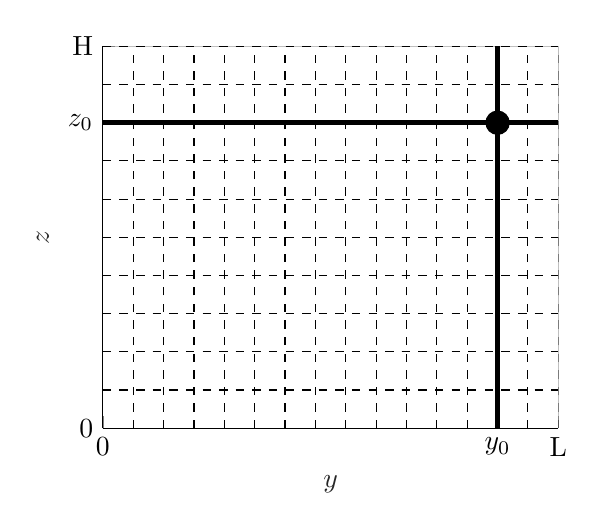
\begin{tikzpicture}

\begin{axis}[%
width=0.477\textwidth,
height=0.4\textwidth,
at={(0\textwidth,0\textwidth)},
scale only axis,
xmin=0,
xmax=15,
xtick={0,13,15},
xticklabels={{0},{$y_0$},{L}},
xlabel style={font=\color{white!15!black}},
xlabel={$y$},
ymin=0,
ymax=5,
ytick={0,4,5},
yticklabels={{0},{$z_0$},{H}},
ylabel style={font=\color{white!15!black}},
ylabel={$z$},
axis background/.style={fill=white},
axis x line*=bottom,
axis y line*=left,
xmajorgrids,
ymajorgrids
]
\addplot [color=black, dashed, forget plot]
  table[row sep=crcr]{%
0	0\\
0	0.0505050505050505\\
0	0.101010101010101\\
0	0.151515151515152\\
0	0.202020202020202\\
0	0.252525252525253\\
0	0.303030303030303\\
0	0.353535353535354\\
0	0.404040404040404\\
0	0.454545454545455\\
0	0.505050505050505\\
0	0.555555555555556\\
0	0.606060606060606\\
0	0.656565656565657\\
0	0.707070707070707\\
0	0.757575757575758\\
0	0.808080808080808\\
0	0.858585858585859\\
0	0.909090909090909\\
0	0.95959595959596\\
0	1.01010101010101\\
0	1.06060606060606\\
0	1.11111111111111\\
0	1.16161616161616\\
0	1.21212121212121\\
0	1.26262626262626\\
0	1.31313131313131\\
0	1.36363636363636\\
0	1.41414141414141\\
0	1.46464646464646\\
0	1.51515151515152\\
0	1.56565656565657\\
0	1.61616161616162\\
0	1.66666666666667\\
0	1.71717171717172\\
0	1.76767676767677\\
0	1.81818181818182\\
0	1.86868686868687\\
0	1.91919191919192\\
0	1.96969696969697\\
0	2.02020202020202\\
0	2.07070707070707\\
0	2.12121212121212\\
0	2.17171717171717\\
0	2.22222222222222\\
0	2.27272727272727\\
0	2.32323232323232\\
0	2.37373737373737\\
0	2.42424242424242\\
0	2.47474747474747\\
0	2.52525252525253\\
0	2.57575757575758\\
0	2.62626262626263\\
0	2.67676767676768\\
0	2.72727272727273\\
0	2.77777777777778\\
0	2.82828282828283\\
0	2.87878787878788\\
0	2.92929292929293\\
0	2.97979797979798\\
0	3.03030303030303\\
0	3.08080808080808\\
0	3.13131313131313\\
0	3.18181818181818\\
0	3.23232323232323\\
0	3.28282828282828\\
0	3.33333333333333\\
0	3.38383838383838\\
0	3.43434343434343\\
0	3.48484848484848\\
0	3.53535353535354\\
0	3.58585858585859\\
0	3.63636363636364\\
0	3.68686868686869\\
0	3.73737373737374\\
0	3.78787878787879\\
0	3.83838383838384\\
0	3.88888888888889\\
0	3.93939393939394\\
0	3.98989898989899\\
0	4.04040404040404\\
0	4.09090909090909\\
0	4.14141414141414\\
0	4.19191919191919\\
0	4.24242424242424\\
0	4.29292929292929\\
0	4.34343434343434\\
0	4.39393939393939\\
0	4.44444444444444\\
0	4.49494949494949\\
0	4.54545454545455\\
0	4.5959595959596\\
0	4.64646464646465\\
0	4.6969696969697\\
0	4.74747474747475\\
0	4.7979797979798\\
0	4.84848484848485\\
0	4.8989898989899\\
0	4.94949494949495\\
0	5\\
};
\addplot [color=black, dashed, forget plot]
  table[row sep=crcr]{%
1	0\\
1	0.0505050505050505\\
1	0.101010101010101\\
1	0.151515151515152\\
1	0.202020202020202\\
1	0.252525252525253\\
1	0.303030303030303\\
1	0.353535353535354\\
1	0.404040404040404\\
1	0.454545454545455\\
1	0.505050505050505\\
1	0.555555555555556\\
1	0.606060606060606\\
1	0.656565656565657\\
1	0.707070707070707\\
1	0.757575757575758\\
1	0.808080808080808\\
1	0.858585858585859\\
1	0.909090909090909\\
1	0.95959595959596\\
1	1.01010101010101\\
1	1.06060606060606\\
1	1.11111111111111\\
1	1.16161616161616\\
1	1.21212121212121\\
1	1.26262626262626\\
1	1.31313131313131\\
1	1.36363636363636\\
1	1.41414141414141\\
1	1.46464646464646\\
1	1.51515151515152\\
1	1.56565656565657\\
1	1.61616161616162\\
1	1.66666666666667\\
1	1.71717171717172\\
1	1.76767676767677\\
1	1.81818181818182\\
1	1.86868686868687\\
1	1.91919191919192\\
1	1.96969696969697\\
1	2.02020202020202\\
1	2.07070707070707\\
1	2.12121212121212\\
1	2.17171717171717\\
1	2.22222222222222\\
1	2.27272727272727\\
1	2.32323232323232\\
1	2.37373737373737\\
1	2.42424242424242\\
1	2.47474747474747\\
1	2.52525252525253\\
1	2.57575757575758\\
1	2.62626262626263\\
1	2.67676767676768\\
1	2.72727272727273\\
1	2.77777777777778\\
1	2.82828282828283\\
1	2.87878787878788\\
1	2.92929292929293\\
1	2.97979797979798\\
1	3.03030303030303\\
1	3.08080808080808\\
1	3.13131313131313\\
1	3.18181818181818\\
1	3.23232323232323\\
1	3.28282828282828\\
1	3.33333333333333\\
1	3.38383838383838\\
1	3.43434343434343\\
1	3.48484848484848\\
1	3.53535353535354\\
1	3.58585858585859\\
1	3.63636363636364\\
1	3.68686868686869\\
1	3.73737373737374\\
1	3.78787878787879\\
1	3.83838383838384\\
1	3.88888888888889\\
1	3.93939393939394\\
1	3.98989898989899\\
1	4.04040404040404\\
1	4.09090909090909\\
1	4.14141414141414\\
1	4.19191919191919\\
1	4.24242424242424\\
1	4.29292929292929\\
1	4.34343434343434\\
1	4.39393939393939\\
1	4.44444444444444\\
1	4.49494949494949\\
1	4.54545454545455\\
1	4.5959595959596\\
1	4.64646464646465\\
1	4.6969696969697\\
1	4.74747474747475\\
1	4.7979797979798\\
1	4.84848484848485\\
1	4.8989898989899\\
1	4.94949494949495\\
1	5\\
};
\addplot [color=black, dashed, forget plot]
  table[row sep=crcr]{%
2	0\\
2	0.0505050505050505\\
2	0.101010101010101\\
2	0.151515151515152\\
2	0.202020202020202\\
2	0.252525252525253\\
2	0.303030303030303\\
2	0.353535353535354\\
2	0.404040404040404\\
2	0.454545454545455\\
2	0.505050505050505\\
2	0.555555555555556\\
2	0.606060606060606\\
2	0.656565656565657\\
2	0.707070707070707\\
2	0.757575757575758\\
2	0.808080808080808\\
2	0.858585858585859\\
2	0.909090909090909\\
2	0.95959595959596\\
2	1.01010101010101\\
2	1.06060606060606\\
2	1.11111111111111\\
2	1.16161616161616\\
2	1.21212121212121\\
2	1.26262626262626\\
2	1.31313131313131\\
2	1.36363636363636\\
2	1.41414141414141\\
2	1.46464646464646\\
2	1.51515151515152\\
2	1.56565656565657\\
2	1.61616161616162\\
2	1.66666666666667\\
2	1.71717171717172\\
2	1.76767676767677\\
2	1.81818181818182\\
2	1.86868686868687\\
2	1.91919191919192\\
2	1.96969696969697\\
2	2.02020202020202\\
2	2.07070707070707\\
2	2.12121212121212\\
2	2.17171717171717\\
2	2.22222222222222\\
2	2.27272727272727\\
2	2.32323232323232\\
2	2.37373737373737\\
2	2.42424242424242\\
2	2.47474747474747\\
2	2.52525252525253\\
2	2.57575757575758\\
2	2.62626262626263\\
2	2.67676767676768\\
2	2.72727272727273\\
2	2.77777777777778\\
2	2.82828282828283\\
2	2.87878787878788\\
2	2.92929292929293\\
2	2.97979797979798\\
2	3.03030303030303\\
2	3.08080808080808\\
2	3.13131313131313\\
2	3.18181818181818\\
2	3.23232323232323\\
2	3.28282828282828\\
2	3.33333333333333\\
2	3.38383838383838\\
2	3.43434343434343\\
2	3.48484848484848\\
2	3.53535353535354\\
2	3.58585858585859\\
2	3.63636363636364\\
2	3.68686868686869\\
2	3.73737373737374\\
2	3.78787878787879\\
2	3.83838383838384\\
2	3.88888888888889\\
2	3.93939393939394\\
2	3.98989898989899\\
2	4.04040404040404\\
2	4.09090909090909\\
2	4.14141414141414\\
2	4.19191919191919\\
2	4.24242424242424\\
2	4.29292929292929\\
2	4.34343434343434\\
2	4.39393939393939\\
2	4.44444444444444\\
2	4.49494949494949\\
2	4.54545454545455\\
2	4.5959595959596\\
2	4.64646464646465\\
2	4.6969696969697\\
2	4.74747474747475\\
2	4.7979797979798\\
2	4.84848484848485\\
2	4.8989898989899\\
2	4.94949494949495\\
2	5\\
};
\addplot [color=black, dashed, forget plot]
  table[row sep=crcr]{%
3	0\\
3	0.0505050505050505\\
3	0.101010101010101\\
3	0.151515151515152\\
3	0.202020202020202\\
3	0.252525252525253\\
3	0.303030303030303\\
3	0.353535353535354\\
3	0.404040404040404\\
3	0.454545454545455\\
3	0.505050505050505\\
3	0.555555555555556\\
3	0.606060606060606\\
3	0.656565656565657\\
3	0.707070707070707\\
3	0.757575757575758\\
3	0.808080808080808\\
3	0.858585858585859\\
3	0.909090909090909\\
3	0.95959595959596\\
3	1.01010101010101\\
3	1.06060606060606\\
3	1.11111111111111\\
3	1.16161616161616\\
3	1.21212121212121\\
3	1.26262626262626\\
3	1.31313131313131\\
3	1.36363636363636\\
3	1.41414141414141\\
3	1.46464646464646\\
3	1.51515151515152\\
3	1.56565656565657\\
3	1.61616161616162\\
3	1.66666666666667\\
3	1.71717171717172\\
3	1.76767676767677\\
3	1.81818181818182\\
3	1.86868686868687\\
3	1.91919191919192\\
3	1.96969696969697\\
3	2.02020202020202\\
3	2.07070707070707\\
3	2.12121212121212\\
3	2.17171717171717\\
3	2.22222222222222\\
3	2.27272727272727\\
3	2.32323232323232\\
3	2.37373737373737\\
3	2.42424242424242\\
3	2.47474747474747\\
3	2.52525252525253\\
3	2.57575757575758\\
3	2.62626262626263\\
3	2.67676767676768\\
3	2.72727272727273\\
3	2.77777777777778\\
3	2.82828282828283\\
3	2.87878787878788\\
3	2.92929292929293\\
3	2.97979797979798\\
3	3.03030303030303\\
3	3.08080808080808\\
3	3.13131313131313\\
3	3.18181818181818\\
3	3.23232323232323\\
3	3.28282828282828\\
3	3.33333333333333\\
3	3.38383838383838\\
3	3.43434343434343\\
3	3.48484848484848\\
3	3.53535353535354\\
3	3.58585858585859\\
3	3.63636363636364\\
3	3.68686868686869\\
3	3.73737373737374\\
3	3.78787878787879\\
3	3.83838383838384\\
3	3.88888888888889\\
3	3.93939393939394\\
3	3.98989898989899\\
3	4.04040404040404\\
3	4.09090909090909\\
3	4.14141414141414\\
3	4.19191919191919\\
3	4.24242424242424\\
3	4.29292929292929\\
3	4.34343434343434\\
3	4.39393939393939\\
3	4.44444444444444\\
3	4.49494949494949\\
3	4.54545454545455\\
3	4.5959595959596\\
3	4.64646464646465\\
3	4.6969696969697\\
3	4.74747474747475\\
3	4.7979797979798\\
3	4.84848484848485\\
3	4.8989898989899\\
3	4.94949494949495\\
3	5\\
};
\addplot [color=black, dashed, forget plot]
  table[row sep=crcr]{%
4	0\\
4	0.0505050505050505\\
4	0.101010101010101\\
4	0.151515151515152\\
4	0.202020202020202\\
4	0.252525252525253\\
4	0.303030303030303\\
4	0.353535353535354\\
4	0.404040404040404\\
4	0.454545454545455\\
4	0.505050505050505\\
4	0.555555555555556\\
4	0.606060606060606\\
4	0.656565656565657\\
4	0.707070707070707\\
4	0.757575757575758\\
4	0.808080808080808\\
4	0.858585858585859\\
4	0.909090909090909\\
4	0.95959595959596\\
4	1.01010101010101\\
4	1.06060606060606\\
4	1.11111111111111\\
4	1.16161616161616\\
4	1.21212121212121\\
4	1.26262626262626\\
4	1.31313131313131\\
4	1.36363636363636\\
4	1.41414141414141\\
4	1.46464646464646\\
4	1.51515151515152\\
4	1.56565656565657\\
4	1.61616161616162\\
4	1.66666666666667\\
4	1.71717171717172\\
4	1.76767676767677\\
4	1.81818181818182\\
4	1.86868686868687\\
4	1.91919191919192\\
4	1.96969696969697\\
4	2.02020202020202\\
4	2.07070707070707\\
4	2.12121212121212\\
4	2.17171717171717\\
4	2.22222222222222\\
4	2.27272727272727\\
4	2.32323232323232\\
4	2.37373737373737\\
4	2.42424242424242\\
4	2.47474747474747\\
4	2.52525252525253\\
4	2.57575757575758\\
4	2.62626262626263\\
4	2.67676767676768\\
4	2.72727272727273\\
4	2.77777777777778\\
4	2.82828282828283\\
4	2.87878787878788\\
4	2.92929292929293\\
4	2.97979797979798\\
4	3.03030303030303\\
4	3.08080808080808\\
4	3.13131313131313\\
4	3.18181818181818\\
4	3.23232323232323\\
4	3.28282828282828\\
4	3.33333333333333\\
4	3.38383838383838\\
4	3.43434343434343\\
4	3.48484848484848\\
4	3.53535353535354\\
4	3.58585858585859\\
4	3.63636363636364\\
4	3.68686868686869\\
4	3.73737373737374\\
4	3.78787878787879\\
4	3.83838383838384\\
4	3.88888888888889\\
4	3.93939393939394\\
4	3.98989898989899\\
4	4.04040404040404\\
4	4.09090909090909\\
4	4.14141414141414\\
4	4.19191919191919\\
4	4.24242424242424\\
4	4.29292929292929\\
4	4.34343434343434\\
4	4.39393939393939\\
4	4.44444444444444\\
4	4.49494949494949\\
4	4.54545454545455\\
4	4.5959595959596\\
4	4.64646464646465\\
4	4.6969696969697\\
4	4.74747474747475\\
4	4.7979797979798\\
4	4.84848484848485\\
4	4.8989898989899\\
4	4.94949494949495\\
4	5\\
};
\addplot [color=black, dashed, forget plot]
  table[row sep=crcr]{%
5	0\\
5	0.0505050505050505\\
5	0.101010101010101\\
5	0.151515151515152\\
5	0.202020202020202\\
5	0.252525252525253\\
5	0.303030303030303\\
5	0.353535353535354\\
5	0.404040404040404\\
5	0.454545454545455\\
5	0.505050505050505\\
5	0.555555555555556\\
5	0.606060606060606\\
5	0.656565656565657\\
5	0.707070707070707\\
5	0.757575757575758\\
5	0.808080808080808\\
5	0.858585858585859\\
5	0.909090909090909\\
5	0.95959595959596\\
5	1.01010101010101\\
5	1.06060606060606\\
5	1.11111111111111\\
5	1.16161616161616\\
5	1.21212121212121\\
5	1.26262626262626\\
5	1.31313131313131\\
5	1.36363636363636\\
5	1.41414141414141\\
5	1.46464646464646\\
5	1.51515151515152\\
5	1.56565656565657\\
5	1.61616161616162\\
5	1.66666666666667\\
5	1.71717171717172\\
5	1.76767676767677\\
5	1.81818181818182\\
5	1.86868686868687\\
5	1.91919191919192\\
5	1.96969696969697\\
5	2.02020202020202\\
5	2.07070707070707\\
5	2.12121212121212\\
5	2.17171717171717\\
5	2.22222222222222\\
5	2.27272727272727\\
5	2.32323232323232\\
5	2.37373737373737\\
5	2.42424242424242\\
5	2.47474747474747\\
5	2.52525252525253\\
5	2.57575757575758\\
5	2.62626262626263\\
5	2.67676767676768\\
5	2.72727272727273\\
5	2.77777777777778\\
5	2.82828282828283\\
5	2.87878787878788\\
5	2.92929292929293\\
5	2.97979797979798\\
5	3.03030303030303\\
5	3.08080808080808\\
5	3.13131313131313\\
5	3.18181818181818\\
5	3.23232323232323\\
5	3.28282828282828\\
5	3.33333333333333\\
5	3.38383838383838\\
5	3.43434343434343\\
5	3.48484848484848\\
5	3.53535353535354\\
5	3.58585858585859\\
5	3.63636363636364\\
5	3.68686868686869\\
5	3.73737373737374\\
5	3.78787878787879\\
5	3.83838383838384\\
5	3.88888888888889\\
5	3.93939393939394\\
5	3.98989898989899\\
5	4.04040404040404\\
5	4.09090909090909\\
5	4.14141414141414\\
5	4.19191919191919\\
5	4.24242424242424\\
5	4.29292929292929\\
5	4.34343434343434\\
5	4.39393939393939\\
5	4.44444444444444\\
5	4.49494949494949\\
5	4.54545454545455\\
5	4.5959595959596\\
5	4.64646464646465\\
5	4.6969696969697\\
5	4.74747474747475\\
5	4.7979797979798\\
5	4.84848484848485\\
5	4.8989898989899\\
5	4.94949494949495\\
5	5\\
};
\addplot [color=black, dashed, forget plot]
  table[row sep=crcr]{%
6	0\\
6	0.0505050505050505\\
6	0.101010101010101\\
6	0.151515151515152\\
6	0.202020202020202\\
6	0.252525252525253\\
6	0.303030303030303\\
6	0.353535353535354\\
6	0.404040404040404\\
6	0.454545454545455\\
6	0.505050505050505\\
6	0.555555555555556\\
6	0.606060606060606\\
6	0.656565656565657\\
6	0.707070707070707\\
6	0.757575757575758\\
6	0.808080808080808\\
6	0.858585858585859\\
6	0.909090909090909\\
6	0.95959595959596\\
6	1.01010101010101\\
6	1.06060606060606\\
6	1.11111111111111\\
6	1.16161616161616\\
6	1.21212121212121\\
6	1.26262626262626\\
6	1.31313131313131\\
6	1.36363636363636\\
6	1.41414141414141\\
6	1.46464646464646\\
6	1.51515151515152\\
6	1.56565656565657\\
6	1.61616161616162\\
6	1.66666666666667\\
6	1.71717171717172\\
6	1.76767676767677\\
6	1.81818181818182\\
6	1.86868686868687\\
6	1.91919191919192\\
6	1.96969696969697\\
6	2.02020202020202\\
6	2.07070707070707\\
6	2.12121212121212\\
6	2.17171717171717\\
6	2.22222222222222\\
6	2.27272727272727\\
6	2.32323232323232\\
6	2.37373737373737\\
6	2.42424242424242\\
6	2.47474747474747\\
6	2.52525252525253\\
6	2.57575757575758\\
6	2.62626262626263\\
6	2.67676767676768\\
6	2.72727272727273\\
6	2.77777777777778\\
6	2.82828282828283\\
6	2.87878787878788\\
6	2.92929292929293\\
6	2.97979797979798\\
6	3.03030303030303\\
6	3.08080808080808\\
6	3.13131313131313\\
6	3.18181818181818\\
6	3.23232323232323\\
6	3.28282828282828\\
6	3.33333333333333\\
6	3.38383838383838\\
6	3.43434343434343\\
6	3.48484848484848\\
6	3.53535353535354\\
6	3.58585858585859\\
6	3.63636363636364\\
6	3.68686868686869\\
6	3.73737373737374\\
6	3.78787878787879\\
6	3.83838383838384\\
6	3.88888888888889\\
6	3.93939393939394\\
6	3.98989898989899\\
6	4.04040404040404\\
6	4.09090909090909\\
6	4.14141414141414\\
6	4.19191919191919\\
6	4.24242424242424\\
6	4.29292929292929\\
6	4.34343434343434\\
6	4.39393939393939\\
6	4.44444444444444\\
6	4.49494949494949\\
6	4.54545454545455\\
6	4.5959595959596\\
6	4.64646464646465\\
6	4.6969696969697\\
6	4.74747474747475\\
6	4.7979797979798\\
6	4.84848484848485\\
6	4.8989898989899\\
6	4.94949494949495\\
6	5\\
};
\addplot [color=black, dashed, forget plot]
  table[row sep=crcr]{%
7	0\\
7	0.0505050505050505\\
7	0.101010101010101\\
7	0.151515151515152\\
7	0.202020202020202\\
7	0.252525252525253\\
7	0.303030303030303\\
7	0.353535353535354\\
7	0.404040404040404\\
7	0.454545454545455\\
7	0.505050505050505\\
7	0.555555555555556\\
7	0.606060606060606\\
7	0.656565656565657\\
7	0.707070707070707\\
7	0.757575757575758\\
7	0.808080808080808\\
7	0.858585858585859\\
7	0.909090909090909\\
7	0.95959595959596\\
7	1.01010101010101\\
7	1.06060606060606\\
7	1.11111111111111\\
7	1.16161616161616\\
7	1.21212121212121\\
7	1.26262626262626\\
7	1.31313131313131\\
7	1.36363636363636\\
7	1.41414141414141\\
7	1.46464646464646\\
7	1.51515151515152\\
7	1.56565656565657\\
7	1.61616161616162\\
7	1.66666666666667\\
7	1.71717171717172\\
7	1.76767676767677\\
7	1.81818181818182\\
7	1.86868686868687\\
7	1.91919191919192\\
7	1.96969696969697\\
7	2.02020202020202\\
7	2.07070707070707\\
7	2.12121212121212\\
7	2.17171717171717\\
7	2.22222222222222\\
7	2.27272727272727\\
7	2.32323232323232\\
7	2.37373737373737\\
7	2.42424242424242\\
7	2.47474747474747\\
7	2.52525252525253\\
7	2.57575757575758\\
7	2.62626262626263\\
7	2.67676767676768\\
7	2.72727272727273\\
7	2.77777777777778\\
7	2.82828282828283\\
7	2.87878787878788\\
7	2.92929292929293\\
7	2.97979797979798\\
7	3.03030303030303\\
7	3.08080808080808\\
7	3.13131313131313\\
7	3.18181818181818\\
7	3.23232323232323\\
7	3.28282828282828\\
7	3.33333333333333\\
7	3.38383838383838\\
7	3.43434343434343\\
7	3.48484848484848\\
7	3.53535353535354\\
7	3.58585858585859\\
7	3.63636363636364\\
7	3.68686868686869\\
7	3.73737373737374\\
7	3.78787878787879\\
7	3.83838383838384\\
7	3.88888888888889\\
7	3.93939393939394\\
7	3.98989898989899\\
7	4.04040404040404\\
7	4.09090909090909\\
7	4.14141414141414\\
7	4.19191919191919\\
7	4.24242424242424\\
7	4.29292929292929\\
7	4.34343434343434\\
7	4.39393939393939\\
7	4.44444444444444\\
7	4.49494949494949\\
7	4.54545454545455\\
7	4.5959595959596\\
7	4.64646464646465\\
7	4.6969696969697\\
7	4.74747474747475\\
7	4.7979797979798\\
7	4.84848484848485\\
7	4.8989898989899\\
7	4.94949494949495\\
7	5\\
};
\addplot [color=black, dashed, forget plot]
  table[row sep=crcr]{%
8	0\\
8	0.0505050505050505\\
8	0.101010101010101\\
8	0.151515151515152\\
8	0.202020202020202\\
8	0.252525252525253\\
8	0.303030303030303\\
8	0.353535353535354\\
8	0.404040404040404\\
8	0.454545454545455\\
8	0.505050505050505\\
8	0.555555555555556\\
8	0.606060606060606\\
8	0.656565656565657\\
8	0.707070707070707\\
8	0.757575757575758\\
8	0.808080808080808\\
8	0.858585858585859\\
8	0.909090909090909\\
8	0.95959595959596\\
8	1.01010101010101\\
8	1.06060606060606\\
8	1.11111111111111\\
8	1.16161616161616\\
8	1.21212121212121\\
8	1.26262626262626\\
8	1.31313131313131\\
8	1.36363636363636\\
8	1.41414141414141\\
8	1.46464646464646\\
8	1.51515151515152\\
8	1.56565656565657\\
8	1.61616161616162\\
8	1.66666666666667\\
8	1.71717171717172\\
8	1.76767676767677\\
8	1.81818181818182\\
8	1.86868686868687\\
8	1.91919191919192\\
8	1.96969696969697\\
8	2.02020202020202\\
8	2.07070707070707\\
8	2.12121212121212\\
8	2.17171717171717\\
8	2.22222222222222\\
8	2.27272727272727\\
8	2.32323232323232\\
8	2.37373737373737\\
8	2.42424242424242\\
8	2.47474747474747\\
8	2.52525252525253\\
8	2.57575757575758\\
8	2.62626262626263\\
8	2.67676767676768\\
8	2.72727272727273\\
8	2.77777777777778\\
8	2.82828282828283\\
8	2.87878787878788\\
8	2.92929292929293\\
8	2.97979797979798\\
8	3.03030303030303\\
8	3.08080808080808\\
8	3.13131313131313\\
8	3.18181818181818\\
8	3.23232323232323\\
8	3.28282828282828\\
8	3.33333333333333\\
8	3.38383838383838\\
8	3.43434343434343\\
8	3.48484848484848\\
8	3.53535353535354\\
8	3.58585858585859\\
8	3.63636363636364\\
8	3.68686868686869\\
8	3.73737373737374\\
8	3.78787878787879\\
8	3.83838383838384\\
8	3.88888888888889\\
8	3.93939393939394\\
8	3.98989898989899\\
8	4.04040404040404\\
8	4.09090909090909\\
8	4.14141414141414\\
8	4.19191919191919\\
8	4.24242424242424\\
8	4.29292929292929\\
8	4.34343434343434\\
8	4.39393939393939\\
8	4.44444444444444\\
8	4.49494949494949\\
8	4.54545454545455\\
8	4.5959595959596\\
8	4.64646464646465\\
8	4.6969696969697\\
8	4.74747474747475\\
8	4.7979797979798\\
8	4.84848484848485\\
8	4.8989898989899\\
8	4.94949494949495\\
8	5\\
};
\addplot [color=black, dashed, forget plot]
  table[row sep=crcr]{%
9	0\\
9	0.0505050505050505\\
9	0.101010101010101\\
9	0.151515151515152\\
9	0.202020202020202\\
9	0.252525252525253\\
9	0.303030303030303\\
9	0.353535353535354\\
9	0.404040404040404\\
9	0.454545454545455\\
9	0.505050505050505\\
9	0.555555555555556\\
9	0.606060606060606\\
9	0.656565656565657\\
9	0.707070707070707\\
9	0.757575757575758\\
9	0.808080808080808\\
9	0.858585858585859\\
9	0.909090909090909\\
9	0.95959595959596\\
9	1.01010101010101\\
9	1.06060606060606\\
9	1.11111111111111\\
9	1.16161616161616\\
9	1.21212121212121\\
9	1.26262626262626\\
9	1.31313131313131\\
9	1.36363636363636\\
9	1.41414141414141\\
9	1.46464646464646\\
9	1.51515151515152\\
9	1.56565656565657\\
9	1.61616161616162\\
9	1.66666666666667\\
9	1.71717171717172\\
9	1.76767676767677\\
9	1.81818181818182\\
9	1.86868686868687\\
9	1.91919191919192\\
9	1.96969696969697\\
9	2.02020202020202\\
9	2.07070707070707\\
9	2.12121212121212\\
9	2.17171717171717\\
9	2.22222222222222\\
9	2.27272727272727\\
9	2.32323232323232\\
9	2.37373737373737\\
9	2.42424242424242\\
9	2.47474747474747\\
9	2.52525252525253\\
9	2.57575757575758\\
9	2.62626262626263\\
9	2.67676767676768\\
9	2.72727272727273\\
9	2.77777777777778\\
9	2.82828282828283\\
9	2.87878787878788\\
9	2.92929292929293\\
9	2.97979797979798\\
9	3.03030303030303\\
9	3.08080808080808\\
9	3.13131313131313\\
9	3.18181818181818\\
9	3.23232323232323\\
9	3.28282828282828\\
9	3.33333333333333\\
9	3.38383838383838\\
9	3.43434343434343\\
9	3.48484848484848\\
9	3.53535353535354\\
9	3.58585858585859\\
9	3.63636363636364\\
9	3.68686868686869\\
9	3.73737373737374\\
9	3.78787878787879\\
9	3.83838383838384\\
9	3.88888888888889\\
9	3.93939393939394\\
9	3.98989898989899\\
9	4.04040404040404\\
9	4.09090909090909\\
9	4.14141414141414\\
9	4.19191919191919\\
9	4.24242424242424\\
9	4.29292929292929\\
9	4.34343434343434\\
9	4.39393939393939\\
9	4.44444444444444\\
9	4.49494949494949\\
9	4.54545454545455\\
9	4.5959595959596\\
9	4.64646464646465\\
9	4.6969696969697\\
9	4.74747474747475\\
9	4.7979797979798\\
9	4.84848484848485\\
9	4.8989898989899\\
9	4.94949494949495\\
9	5\\
};
\addplot [color=black, dashed, forget plot]
  table[row sep=crcr]{%
10	0\\
10	0.0505050505050505\\
10	0.101010101010101\\
10	0.151515151515152\\
10	0.202020202020202\\
10	0.252525252525253\\
10	0.303030303030303\\
10	0.353535353535354\\
10	0.404040404040404\\
10	0.454545454545455\\
10	0.505050505050505\\
10	0.555555555555556\\
10	0.606060606060606\\
10	0.656565656565657\\
10	0.707070707070707\\
10	0.757575757575758\\
10	0.808080808080808\\
10	0.858585858585859\\
10	0.909090909090909\\
10	0.95959595959596\\
10	1.01010101010101\\
10	1.06060606060606\\
10	1.11111111111111\\
10	1.16161616161616\\
10	1.21212121212121\\
10	1.26262626262626\\
10	1.31313131313131\\
10	1.36363636363636\\
10	1.41414141414141\\
10	1.46464646464646\\
10	1.51515151515152\\
10	1.56565656565657\\
10	1.61616161616162\\
10	1.66666666666667\\
10	1.71717171717172\\
10	1.76767676767677\\
10	1.81818181818182\\
10	1.86868686868687\\
10	1.91919191919192\\
10	1.96969696969697\\
10	2.02020202020202\\
10	2.07070707070707\\
10	2.12121212121212\\
10	2.17171717171717\\
10	2.22222222222222\\
10	2.27272727272727\\
10	2.32323232323232\\
10	2.37373737373737\\
10	2.42424242424242\\
10	2.47474747474747\\
10	2.52525252525253\\
10	2.57575757575758\\
10	2.62626262626263\\
10	2.67676767676768\\
10	2.72727272727273\\
10	2.77777777777778\\
10	2.82828282828283\\
10	2.87878787878788\\
10	2.92929292929293\\
10	2.97979797979798\\
10	3.03030303030303\\
10	3.08080808080808\\
10	3.13131313131313\\
10	3.18181818181818\\
10	3.23232323232323\\
10	3.28282828282828\\
10	3.33333333333333\\
10	3.38383838383838\\
10	3.43434343434343\\
10	3.48484848484848\\
10	3.53535353535354\\
10	3.58585858585859\\
10	3.63636363636364\\
10	3.68686868686869\\
10	3.73737373737374\\
10	3.78787878787879\\
10	3.83838383838384\\
10	3.88888888888889\\
10	3.93939393939394\\
10	3.98989898989899\\
10	4.04040404040404\\
10	4.09090909090909\\
10	4.14141414141414\\
10	4.19191919191919\\
10	4.24242424242424\\
10	4.29292929292929\\
10	4.34343434343434\\
10	4.39393939393939\\
10	4.44444444444444\\
10	4.49494949494949\\
10	4.54545454545455\\
10	4.5959595959596\\
10	4.64646464646465\\
10	4.6969696969697\\
10	4.74747474747475\\
10	4.7979797979798\\
10	4.84848484848485\\
10	4.8989898989899\\
10	4.94949494949495\\
10	5\\
};
\addplot [color=black, dashed, forget plot]
  table[row sep=crcr]{%
11	0\\
11	0.0505050505050505\\
11	0.101010101010101\\
11	0.151515151515152\\
11	0.202020202020202\\
11	0.252525252525253\\
11	0.303030303030303\\
11	0.353535353535354\\
11	0.404040404040404\\
11	0.454545454545455\\
11	0.505050505050505\\
11	0.555555555555556\\
11	0.606060606060606\\
11	0.656565656565657\\
11	0.707070707070707\\
11	0.757575757575758\\
11	0.808080808080808\\
11	0.858585858585859\\
11	0.909090909090909\\
11	0.95959595959596\\
11	1.01010101010101\\
11	1.06060606060606\\
11	1.11111111111111\\
11	1.16161616161616\\
11	1.21212121212121\\
11	1.26262626262626\\
11	1.31313131313131\\
11	1.36363636363636\\
11	1.41414141414141\\
11	1.46464646464646\\
11	1.51515151515152\\
11	1.56565656565657\\
11	1.61616161616162\\
11	1.66666666666667\\
11	1.71717171717172\\
11	1.76767676767677\\
11	1.81818181818182\\
11	1.86868686868687\\
11	1.91919191919192\\
11	1.96969696969697\\
11	2.02020202020202\\
11	2.07070707070707\\
11	2.12121212121212\\
11	2.17171717171717\\
11	2.22222222222222\\
11	2.27272727272727\\
11	2.32323232323232\\
11	2.37373737373737\\
11	2.42424242424242\\
11	2.47474747474747\\
11	2.52525252525253\\
11	2.57575757575758\\
11	2.62626262626263\\
11	2.67676767676768\\
11	2.72727272727273\\
11	2.77777777777778\\
11	2.82828282828283\\
11	2.87878787878788\\
11	2.92929292929293\\
11	2.97979797979798\\
11	3.03030303030303\\
11	3.08080808080808\\
11	3.13131313131313\\
11	3.18181818181818\\
11	3.23232323232323\\
11	3.28282828282828\\
11	3.33333333333333\\
11	3.38383838383838\\
11	3.43434343434343\\
11	3.48484848484848\\
11	3.53535353535354\\
11	3.58585858585859\\
11	3.63636363636364\\
11	3.68686868686869\\
11	3.73737373737374\\
11	3.78787878787879\\
11	3.83838383838384\\
11	3.88888888888889\\
11	3.93939393939394\\
11	3.98989898989899\\
11	4.04040404040404\\
11	4.09090909090909\\
11	4.14141414141414\\
11	4.19191919191919\\
11	4.24242424242424\\
11	4.29292929292929\\
11	4.34343434343434\\
11	4.39393939393939\\
11	4.44444444444444\\
11	4.49494949494949\\
11	4.54545454545455\\
11	4.5959595959596\\
11	4.64646464646465\\
11	4.6969696969697\\
11	4.74747474747475\\
11	4.7979797979798\\
11	4.84848484848485\\
11	4.8989898989899\\
11	4.94949494949495\\
11	5\\
};
\addplot [color=black, dashed, forget plot]
  table[row sep=crcr]{%
12	0\\
12	0.0505050505050505\\
12	0.101010101010101\\
12	0.151515151515152\\
12	0.202020202020202\\
12	0.252525252525253\\
12	0.303030303030303\\
12	0.353535353535354\\
12	0.404040404040404\\
12	0.454545454545455\\
12	0.505050505050505\\
12	0.555555555555556\\
12	0.606060606060606\\
12	0.656565656565657\\
12	0.707070707070707\\
12	0.757575757575758\\
12	0.808080808080808\\
12	0.858585858585859\\
12	0.909090909090909\\
12	0.95959595959596\\
12	1.01010101010101\\
12	1.06060606060606\\
12	1.11111111111111\\
12	1.16161616161616\\
12	1.21212121212121\\
12	1.26262626262626\\
12	1.31313131313131\\
12	1.36363636363636\\
12	1.41414141414141\\
12	1.46464646464646\\
12	1.51515151515152\\
12	1.56565656565657\\
12	1.61616161616162\\
12	1.66666666666667\\
12	1.71717171717172\\
12	1.76767676767677\\
12	1.81818181818182\\
12	1.86868686868687\\
12	1.91919191919192\\
12	1.96969696969697\\
12	2.02020202020202\\
12	2.07070707070707\\
12	2.12121212121212\\
12	2.17171717171717\\
12	2.22222222222222\\
12	2.27272727272727\\
12	2.32323232323232\\
12	2.37373737373737\\
12	2.42424242424242\\
12	2.47474747474747\\
12	2.52525252525253\\
12	2.57575757575758\\
12	2.62626262626263\\
12	2.67676767676768\\
12	2.72727272727273\\
12	2.77777777777778\\
12	2.82828282828283\\
12	2.87878787878788\\
12	2.92929292929293\\
12	2.97979797979798\\
12	3.03030303030303\\
12	3.08080808080808\\
12	3.13131313131313\\
12	3.18181818181818\\
12	3.23232323232323\\
12	3.28282828282828\\
12	3.33333333333333\\
12	3.38383838383838\\
12	3.43434343434343\\
12	3.48484848484848\\
12	3.53535353535354\\
12	3.58585858585859\\
12	3.63636363636364\\
12	3.68686868686869\\
12	3.73737373737374\\
12	3.78787878787879\\
12	3.83838383838384\\
12	3.88888888888889\\
12	3.93939393939394\\
12	3.98989898989899\\
12	4.04040404040404\\
12	4.09090909090909\\
12	4.14141414141414\\
12	4.19191919191919\\
12	4.24242424242424\\
12	4.29292929292929\\
12	4.34343434343434\\
12	4.39393939393939\\
12	4.44444444444444\\
12	4.49494949494949\\
12	4.54545454545455\\
12	4.5959595959596\\
12	4.64646464646465\\
12	4.6969696969697\\
12	4.74747474747475\\
12	4.7979797979798\\
12	4.84848484848485\\
12	4.8989898989899\\
12	4.94949494949495\\
12	5\\
};
\addplot [color=black, dashed, forget plot]
  table[row sep=crcr]{%
13	0\\
13	0.0505050505050505\\
13	0.101010101010101\\
13	0.151515151515152\\
13	0.202020202020202\\
13	0.252525252525253\\
13	0.303030303030303\\
13	0.353535353535354\\
13	0.404040404040404\\
13	0.454545454545455\\
13	0.505050505050505\\
13	0.555555555555556\\
13	0.606060606060606\\
13	0.656565656565657\\
13	0.707070707070707\\
13	0.757575757575758\\
13	0.808080808080808\\
13	0.858585858585859\\
13	0.909090909090909\\
13	0.95959595959596\\
13	1.01010101010101\\
13	1.06060606060606\\
13	1.11111111111111\\
13	1.16161616161616\\
13	1.21212121212121\\
13	1.26262626262626\\
13	1.31313131313131\\
13	1.36363636363636\\
13	1.41414141414141\\
13	1.46464646464646\\
13	1.51515151515152\\
13	1.56565656565657\\
13	1.61616161616162\\
13	1.66666666666667\\
13	1.71717171717172\\
13	1.76767676767677\\
13	1.81818181818182\\
13	1.86868686868687\\
13	1.91919191919192\\
13	1.96969696969697\\
13	2.02020202020202\\
13	2.07070707070707\\
13	2.12121212121212\\
13	2.17171717171717\\
13	2.22222222222222\\
13	2.27272727272727\\
13	2.32323232323232\\
13	2.37373737373737\\
13	2.42424242424242\\
13	2.47474747474747\\
13	2.52525252525253\\
13	2.57575757575758\\
13	2.62626262626263\\
13	2.67676767676768\\
13	2.72727272727273\\
13	2.77777777777778\\
13	2.82828282828283\\
13	2.87878787878788\\
13	2.92929292929293\\
13	2.97979797979798\\
13	3.03030303030303\\
13	3.08080808080808\\
13	3.13131313131313\\
13	3.18181818181818\\
13	3.23232323232323\\
13	3.28282828282828\\
13	3.33333333333333\\
13	3.38383838383838\\
13	3.43434343434343\\
13	3.48484848484848\\
13	3.53535353535354\\
13	3.58585858585859\\
13	3.63636363636364\\
13	3.68686868686869\\
13	3.73737373737374\\
13	3.78787878787879\\
13	3.83838383838384\\
13	3.88888888888889\\
13	3.93939393939394\\
13	3.98989898989899\\
13	4.04040404040404\\
13	4.09090909090909\\
13	4.14141414141414\\
13	4.19191919191919\\
13	4.24242424242424\\
13	4.29292929292929\\
13	4.34343434343434\\
13	4.39393939393939\\
13	4.44444444444444\\
13	4.49494949494949\\
13	4.54545454545455\\
13	4.5959595959596\\
13	4.64646464646465\\
13	4.6969696969697\\
13	4.74747474747475\\
13	4.7979797979798\\
13	4.84848484848485\\
13	4.8989898989899\\
13	4.94949494949495\\
13	5\\
};
\addplot [color=black, dashed, forget plot]
  table[row sep=crcr]{%
14	0\\
14	0.0505050505050505\\
14	0.101010101010101\\
14	0.151515151515152\\
14	0.202020202020202\\
14	0.252525252525253\\
14	0.303030303030303\\
14	0.353535353535354\\
14	0.404040404040404\\
14	0.454545454545455\\
14	0.505050505050505\\
14	0.555555555555556\\
14	0.606060606060606\\
14	0.656565656565657\\
14	0.707070707070707\\
14	0.757575757575758\\
14	0.808080808080808\\
14	0.858585858585859\\
14	0.909090909090909\\
14	0.95959595959596\\
14	1.01010101010101\\
14	1.06060606060606\\
14	1.11111111111111\\
14	1.16161616161616\\
14	1.21212121212121\\
14	1.26262626262626\\
14	1.31313131313131\\
14	1.36363636363636\\
14	1.41414141414141\\
14	1.46464646464646\\
14	1.51515151515152\\
14	1.56565656565657\\
14	1.61616161616162\\
14	1.66666666666667\\
14	1.71717171717172\\
14	1.76767676767677\\
14	1.81818181818182\\
14	1.86868686868687\\
14	1.91919191919192\\
14	1.96969696969697\\
14	2.02020202020202\\
14	2.07070707070707\\
14	2.12121212121212\\
14	2.17171717171717\\
14	2.22222222222222\\
14	2.27272727272727\\
14	2.32323232323232\\
14	2.37373737373737\\
14	2.42424242424242\\
14	2.47474747474747\\
14	2.52525252525253\\
14	2.57575757575758\\
14	2.62626262626263\\
14	2.67676767676768\\
14	2.72727272727273\\
14	2.77777777777778\\
14	2.82828282828283\\
14	2.87878787878788\\
14	2.92929292929293\\
14	2.97979797979798\\
14	3.03030303030303\\
14	3.08080808080808\\
14	3.13131313131313\\
14	3.18181818181818\\
14	3.23232323232323\\
14	3.28282828282828\\
14	3.33333333333333\\
14	3.38383838383838\\
14	3.43434343434343\\
14	3.48484848484848\\
14	3.53535353535354\\
14	3.58585858585859\\
14	3.63636363636364\\
14	3.68686868686869\\
14	3.73737373737374\\
14	3.78787878787879\\
14	3.83838383838384\\
14	3.88888888888889\\
14	3.93939393939394\\
14	3.98989898989899\\
14	4.04040404040404\\
14	4.09090909090909\\
14	4.14141414141414\\
14	4.19191919191919\\
14	4.24242424242424\\
14	4.29292929292929\\
14	4.34343434343434\\
14	4.39393939393939\\
14	4.44444444444444\\
14	4.49494949494949\\
14	4.54545454545455\\
14	4.5959595959596\\
14	4.64646464646465\\
14	4.6969696969697\\
14	4.74747474747475\\
14	4.7979797979798\\
14	4.84848484848485\\
14	4.8989898989899\\
14	4.94949494949495\\
14	5\\
};
\addplot [color=black, dashed, forget plot]
  table[row sep=crcr]{%
15	0\\
15	0.0505050505050505\\
15	0.101010101010101\\
15	0.151515151515152\\
15	0.202020202020202\\
15	0.252525252525253\\
15	0.303030303030303\\
15	0.353535353535354\\
15	0.404040404040404\\
15	0.454545454545455\\
15	0.505050505050505\\
15	0.555555555555556\\
15	0.606060606060606\\
15	0.656565656565657\\
15	0.707070707070707\\
15	0.757575757575758\\
15	0.808080808080808\\
15	0.858585858585859\\
15	0.909090909090909\\
15	0.95959595959596\\
15	1.01010101010101\\
15	1.06060606060606\\
15	1.11111111111111\\
15	1.16161616161616\\
15	1.21212121212121\\
15	1.26262626262626\\
15	1.31313131313131\\
15	1.36363636363636\\
15	1.41414141414141\\
15	1.46464646464646\\
15	1.51515151515152\\
15	1.56565656565657\\
15	1.61616161616162\\
15	1.66666666666667\\
15	1.71717171717172\\
15	1.76767676767677\\
15	1.81818181818182\\
15	1.86868686868687\\
15	1.91919191919192\\
15	1.96969696969697\\
15	2.02020202020202\\
15	2.07070707070707\\
15	2.12121212121212\\
15	2.17171717171717\\
15	2.22222222222222\\
15	2.27272727272727\\
15	2.32323232323232\\
15	2.37373737373737\\
15	2.42424242424242\\
15	2.47474747474747\\
15	2.52525252525253\\
15	2.57575757575758\\
15	2.62626262626263\\
15	2.67676767676768\\
15	2.72727272727273\\
15	2.77777777777778\\
15	2.82828282828283\\
15	2.87878787878788\\
15	2.92929292929293\\
15	2.97979797979798\\
15	3.03030303030303\\
15	3.08080808080808\\
15	3.13131313131313\\
15	3.18181818181818\\
15	3.23232323232323\\
15	3.28282828282828\\
15	3.33333333333333\\
15	3.38383838383838\\
15	3.43434343434343\\
15	3.48484848484848\\
15	3.53535353535354\\
15	3.58585858585859\\
15	3.63636363636364\\
15	3.68686868686869\\
15	3.73737373737374\\
15	3.78787878787879\\
15	3.83838383838384\\
15	3.88888888888889\\
15	3.93939393939394\\
15	3.98989898989899\\
15	4.04040404040404\\
15	4.09090909090909\\
15	4.14141414141414\\
15	4.19191919191919\\
15	4.24242424242424\\
15	4.29292929292929\\
15	4.34343434343434\\
15	4.39393939393939\\
15	4.44444444444444\\
15	4.49494949494949\\
15	4.54545454545455\\
15	4.5959595959596\\
15	4.64646464646465\\
15	4.6969696969697\\
15	4.74747474747475\\
15	4.7979797979798\\
15	4.84848484848485\\
15	4.8989898989899\\
15	4.94949494949495\\
15	5\\
};
\addplot [color=black, dashed, forget plot]
  table[row sep=crcr]{%
0	0\\
0.151515151515152	0\\
0.303030303030303	0\\
0.454545454545455	0\\
0.606060606060606	0\\
0.757575757575758	0\\
0.909090909090909	0\\
1.06060606060606	0\\
1.21212121212121	0\\
1.36363636363636	0\\
1.51515151515152	0\\
1.66666666666667	0\\
1.81818181818182	0\\
1.96969696969697	0\\
2.12121212121212	0\\
2.27272727272727	0\\
2.42424242424242	0\\
2.57575757575758	0\\
2.72727272727273	0\\
2.87878787878788	0\\
3.03030303030303	0\\
3.18181818181818	0\\
3.33333333333333	0\\
3.48484848484848	0\\
3.63636363636364	0\\
3.78787878787879	0\\
3.93939393939394	0\\
4.09090909090909	0\\
4.24242424242424	0\\
4.39393939393939	0\\
4.54545454545455	0\\
4.6969696969697	0\\
4.84848484848485	0\\
5	0\\
5.15151515151515	0\\
5.3030303030303	0\\
5.45454545454545	0\\
5.60606060606061	0\\
5.75757575757576	0\\
5.90909090909091	0\\
6.06060606060606	0\\
6.21212121212121	0\\
6.36363636363636	0\\
6.51515151515152	0\\
6.66666666666667	0\\
6.81818181818182	0\\
6.96969696969697	0\\
7.12121212121212	0\\
7.27272727272727	0\\
7.42424242424242	0\\
7.57575757575758	0\\
7.72727272727273	0\\
7.87878787878788	0\\
8.03030303030303	0\\
8.18181818181818	0\\
8.33333333333333	0\\
8.48484848484848	0\\
8.63636363636364	0\\
8.78787878787879	0\\
8.93939393939394	0\\
9.09090909090909	0\\
9.24242424242424	0\\
9.39393939393939	0\\
9.54545454545454	0\\
9.6969696969697	0\\
9.84848484848485	0\\
10	0\\
10.1515151515152	0\\
10.3030303030303	0\\
10.4545454545455	0\\
10.6060606060606	0\\
10.7575757575758	0\\
10.9090909090909	0\\
11.0606060606061	0\\
11.2121212121212	0\\
11.3636363636364	0\\
11.5151515151515	0\\
11.6666666666667	0\\
11.8181818181818	0\\
11.969696969697	0\\
12.1212121212121	0\\
12.2727272727273	0\\
12.4242424242424	0\\
12.5757575757576	0\\
12.7272727272727	0\\
12.8787878787879	0\\
13.030303030303	0\\
13.1818181818182	0\\
13.3333333333333	0\\
13.4848484848485	0\\
13.6363636363636	0\\
13.7878787878788	0\\
13.9393939393939	0\\
14.0909090909091	0\\
14.2424242424242	0\\
14.3939393939394	0\\
14.5454545454545	0\\
14.6969696969697	0\\
14.8484848484848	0\\
15	0\\
};
\addplot [color=black, dashed, forget plot]
  table[row sep=crcr]{%
0	0.5\\
0.151515151515152	0.5\\
0.303030303030303	0.5\\
0.454545454545455	0.5\\
0.606060606060606	0.5\\
0.757575757575758	0.5\\
0.909090909090909	0.5\\
1.06060606060606	0.5\\
1.21212121212121	0.5\\
1.36363636363636	0.5\\
1.51515151515152	0.5\\
1.66666666666667	0.5\\
1.81818181818182	0.5\\
1.96969696969697	0.5\\
2.12121212121212	0.5\\
2.27272727272727	0.5\\
2.42424242424242	0.5\\
2.57575757575758	0.5\\
2.72727272727273	0.5\\
2.87878787878788	0.5\\
3.03030303030303	0.5\\
3.18181818181818	0.5\\
3.33333333333333	0.5\\
3.48484848484848	0.5\\
3.63636363636364	0.5\\
3.78787878787879	0.5\\
3.93939393939394	0.5\\
4.09090909090909	0.5\\
4.24242424242424	0.5\\
4.39393939393939	0.5\\
4.54545454545455	0.5\\
4.6969696969697	0.5\\
4.84848484848485	0.5\\
5	0.5\\
5.15151515151515	0.5\\
5.3030303030303	0.5\\
5.45454545454545	0.5\\
5.60606060606061	0.5\\
5.75757575757576	0.5\\
5.90909090909091	0.5\\
6.06060606060606	0.5\\
6.21212121212121	0.5\\
6.36363636363636	0.5\\
6.51515151515152	0.5\\
6.66666666666667	0.5\\
6.81818181818182	0.5\\
6.96969696969697	0.5\\
7.12121212121212	0.5\\
7.27272727272727	0.5\\
7.42424242424242	0.5\\
7.57575757575758	0.5\\
7.72727272727273	0.5\\
7.87878787878788	0.5\\
8.03030303030303	0.5\\
8.18181818181818	0.5\\
8.33333333333333	0.5\\
8.48484848484848	0.5\\
8.63636363636364	0.5\\
8.78787878787879	0.5\\
8.93939393939394	0.5\\
9.09090909090909	0.5\\
9.24242424242424	0.5\\
9.39393939393939	0.5\\
9.54545454545454	0.5\\
9.6969696969697	0.5\\
9.84848484848485	0.5\\
10	0.5\\
10.1515151515152	0.5\\
10.3030303030303	0.5\\
10.4545454545455	0.5\\
10.6060606060606	0.5\\
10.7575757575758	0.5\\
10.9090909090909	0.5\\
11.0606060606061	0.5\\
11.2121212121212	0.5\\
11.3636363636364	0.5\\
11.5151515151515	0.5\\
11.6666666666667	0.5\\
11.8181818181818	0.5\\
11.969696969697	0.5\\
12.1212121212121	0.5\\
12.2727272727273	0.5\\
12.4242424242424	0.5\\
12.5757575757576	0.5\\
12.7272727272727	0.5\\
12.8787878787879	0.5\\
13.030303030303	0.5\\
13.1818181818182	0.5\\
13.3333333333333	0.5\\
13.4848484848485	0.5\\
13.6363636363636	0.5\\
13.7878787878788	0.5\\
13.9393939393939	0.5\\
14.0909090909091	0.5\\
14.2424242424242	0.5\\
14.3939393939394	0.5\\
14.5454545454545	0.5\\
14.6969696969697	0.5\\
14.8484848484848	0.5\\
15	0.5\\
};
\addplot [color=black, dashed, forget plot]
  table[row sep=crcr]{%
0	1\\
0.151515151515152	1\\
0.303030303030303	1\\
0.454545454545455	1\\
0.606060606060606	1\\
0.757575757575758	1\\
0.909090909090909	1\\
1.06060606060606	1\\
1.21212121212121	1\\
1.36363636363636	1\\
1.51515151515152	1\\
1.66666666666667	1\\
1.81818181818182	1\\
1.96969696969697	1\\
2.12121212121212	1\\
2.27272727272727	1\\
2.42424242424242	1\\
2.57575757575758	1\\
2.72727272727273	1\\
2.87878787878788	1\\
3.03030303030303	1\\
3.18181818181818	1\\
3.33333333333333	1\\
3.48484848484848	1\\
3.63636363636364	1\\
3.78787878787879	1\\
3.93939393939394	1\\
4.09090909090909	1\\
4.24242424242424	1\\
4.39393939393939	1\\
4.54545454545455	1\\
4.6969696969697	1\\
4.84848484848485	1\\
5	1\\
5.15151515151515	1\\
5.3030303030303	1\\
5.45454545454545	1\\
5.60606060606061	1\\
5.75757575757576	1\\
5.90909090909091	1\\
6.06060606060606	1\\
6.21212121212121	1\\
6.36363636363636	1\\
6.51515151515152	1\\
6.66666666666667	1\\
6.81818181818182	1\\
6.96969696969697	1\\
7.12121212121212	1\\
7.27272727272727	1\\
7.42424242424242	1\\
7.57575757575758	1\\
7.72727272727273	1\\
7.87878787878788	1\\
8.03030303030303	1\\
8.18181818181818	1\\
8.33333333333333	1\\
8.48484848484848	1\\
8.63636363636364	1\\
8.78787878787879	1\\
8.93939393939394	1\\
9.09090909090909	1\\
9.24242424242424	1\\
9.39393939393939	1\\
9.54545454545454	1\\
9.6969696969697	1\\
9.84848484848485	1\\
10	1\\
10.1515151515152	1\\
10.3030303030303	1\\
10.4545454545455	1\\
10.6060606060606	1\\
10.7575757575758	1\\
10.9090909090909	1\\
11.0606060606061	1\\
11.2121212121212	1\\
11.3636363636364	1\\
11.5151515151515	1\\
11.6666666666667	1\\
11.8181818181818	1\\
11.969696969697	1\\
12.1212121212121	1\\
12.2727272727273	1\\
12.4242424242424	1\\
12.5757575757576	1\\
12.7272727272727	1\\
12.8787878787879	1\\
13.030303030303	1\\
13.1818181818182	1\\
13.3333333333333	1\\
13.4848484848485	1\\
13.6363636363636	1\\
13.7878787878788	1\\
13.9393939393939	1\\
14.0909090909091	1\\
14.2424242424242	1\\
14.3939393939394	1\\
14.5454545454545	1\\
14.6969696969697	1\\
14.8484848484848	1\\
15	1\\
};
\addplot [color=black, dashed, forget plot]
  table[row sep=crcr]{%
0	1.5\\
0.151515151515152	1.5\\
0.303030303030303	1.5\\
0.454545454545455	1.5\\
0.606060606060606	1.5\\
0.757575757575758	1.5\\
0.909090909090909	1.5\\
1.06060606060606	1.5\\
1.21212121212121	1.5\\
1.36363636363636	1.5\\
1.51515151515152	1.5\\
1.66666666666667	1.5\\
1.81818181818182	1.5\\
1.96969696969697	1.5\\
2.12121212121212	1.5\\
2.27272727272727	1.5\\
2.42424242424242	1.5\\
2.57575757575758	1.5\\
2.72727272727273	1.5\\
2.87878787878788	1.5\\
3.03030303030303	1.5\\
3.18181818181818	1.5\\
3.33333333333333	1.5\\
3.48484848484848	1.5\\
3.63636363636364	1.5\\
3.78787878787879	1.5\\
3.93939393939394	1.5\\
4.09090909090909	1.5\\
4.24242424242424	1.5\\
4.39393939393939	1.5\\
4.54545454545455	1.5\\
4.6969696969697	1.5\\
4.84848484848485	1.5\\
5	1.5\\
5.15151515151515	1.5\\
5.3030303030303	1.5\\
5.45454545454545	1.5\\
5.60606060606061	1.5\\
5.75757575757576	1.5\\
5.90909090909091	1.5\\
6.06060606060606	1.5\\
6.21212121212121	1.5\\
6.36363636363636	1.5\\
6.51515151515152	1.5\\
6.66666666666667	1.5\\
6.81818181818182	1.5\\
6.96969696969697	1.5\\
7.12121212121212	1.5\\
7.27272727272727	1.5\\
7.42424242424242	1.5\\
7.57575757575758	1.5\\
7.72727272727273	1.5\\
7.87878787878788	1.5\\
8.03030303030303	1.5\\
8.18181818181818	1.5\\
8.33333333333333	1.5\\
8.48484848484848	1.5\\
8.63636363636364	1.5\\
8.78787878787879	1.5\\
8.93939393939394	1.5\\
9.09090909090909	1.5\\
9.24242424242424	1.5\\
9.39393939393939	1.5\\
9.54545454545454	1.5\\
9.6969696969697	1.5\\
9.84848484848485	1.5\\
10	1.5\\
10.1515151515152	1.5\\
10.3030303030303	1.5\\
10.4545454545455	1.5\\
10.6060606060606	1.5\\
10.7575757575758	1.5\\
10.9090909090909	1.5\\
11.0606060606061	1.5\\
11.2121212121212	1.5\\
11.3636363636364	1.5\\
11.5151515151515	1.5\\
11.6666666666667	1.5\\
11.8181818181818	1.5\\
11.969696969697	1.5\\
12.1212121212121	1.5\\
12.2727272727273	1.5\\
12.4242424242424	1.5\\
12.5757575757576	1.5\\
12.7272727272727	1.5\\
12.8787878787879	1.5\\
13.030303030303	1.5\\
13.1818181818182	1.5\\
13.3333333333333	1.5\\
13.4848484848485	1.5\\
13.6363636363636	1.5\\
13.7878787878788	1.5\\
13.9393939393939	1.5\\
14.0909090909091	1.5\\
14.2424242424242	1.5\\
14.3939393939394	1.5\\
14.5454545454545	1.5\\
14.6969696969697	1.5\\
14.8484848484848	1.5\\
15	1.5\\
};
\addplot [color=black, dashed, forget plot]
  table[row sep=crcr]{%
0	2\\
0.151515151515152	2\\
0.303030303030303	2\\
0.454545454545455	2\\
0.606060606060606	2\\
0.757575757575758	2\\
0.909090909090909	2\\
1.06060606060606	2\\
1.21212121212121	2\\
1.36363636363636	2\\
1.51515151515152	2\\
1.66666666666667	2\\
1.81818181818182	2\\
1.96969696969697	2\\
2.12121212121212	2\\
2.27272727272727	2\\
2.42424242424242	2\\
2.57575757575758	2\\
2.72727272727273	2\\
2.87878787878788	2\\
3.03030303030303	2\\
3.18181818181818	2\\
3.33333333333333	2\\
3.48484848484848	2\\
3.63636363636364	2\\
3.78787878787879	2\\
3.93939393939394	2\\
4.09090909090909	2\\
4.24242424242424	2\\
4.39393939393939	2\\
4.54545454545455	2\\
4.6969696969697	2\\
4.84848484848485	2\\
5	2\\
5.15151515151515	2\\
5.3030303030303	2\\
5.45454545454545	2\\
5.60606060606061	2\\
5.75757575757576	2\\
5.90909090909091	2\\
6.06060606060606	2\\
6.21212121212121	2\\
6.36363636363636	2\\
6.51515151515152	2\\
6.66666666666667	2\\
6.81818181818182	2\\
6.96969696969697	2\\
7.12121212121212	2\\
7.27272727272727	2\\
7.42424242424242	2\\
7.57575757575758	2\\
7.72727272727273	2\\
7.87878787878788	2\\
8.03030303030303	2\\
8.18181818181818	2\\
8.33333333333333	2\\
8.48484848484848	2\\
8.63636363636364	2\\
8.78787878787879	2\\
8.93939393939394	2\\
9.09090909090909	2\\
9.24242424242424	2\\
9.39393939393939	2\\
9.54545454545454	2\\
9.6969696969697	2\\
9.84848484848485	2\\
10	2\\
10.1515151515152	2\\
10.3030303030303	2\\
10.4545454545455	2\\
10.6060606060606	2\\
10.7575757575758	2\\
10.9090909090909	2\\
11.0606060606061	2\\
11.2121212121212	2\\
11.3636363636364	2\\
11.5151515151515	2\\
11.6666666666667	2\\
11.8181818181818	2\\
11.969696969697	2\\
12.1212121212121	2\\
12.2727272727273	2\\
12.4242424242424	2\\
12.5757575757576	2\\
12.7272727272727	2\\
12.8787878787879	2\\
13.030303030303	2\\
13.1818181818182	2\\
13.3333333333333	2\\
13.4848484848485	2\\
13.6363636363636	2\\
13.7878787878788	2\\
13.9393939393939	2\\
14.0909090909091	2\\
14.2424242424242	2\\
14.3939393939394	2\\
14.5454545454545	2\\
14.6969696969697	2\\
14.8484848484848	2\\
15	2\\
};
\addplot [color=black, dashed, forget plot]
  table[row sep=crcr]{%
0	2.5\\
0.151515151515152	2.5\\
0.303030303030303	2.5\\
0.454545454545455	2.5\\
0.606060606060606	2.5\\
0.757575757575758	2.5\\
0.909090909090909	2.5\\
1.06060606060606	2.5\\
1.21212121212121	2.5\\
1.36363636363636	2.5\\
1.51515151515152	2.5\\
1.66666666666667	2.5\\
1.81818181818182	2.5\\
1.96969696969697	2.5\\
2.12121212121212	2.5\\
2.27272727272727	2.5\\
2.42424242424242	2.5\\
2.57575757575758	2.5\\
2.72727272727273	2.5\\
2.87878787878788	2.5\\
3.03030303030303	2.5\\
3.18181818181818	2.5\\
3.33333333333333	2.5\\
3.48484848484848	2.5\\
3.63636363636364	2.5\\
3.78787878787879	2.5\\
3.93939393939394	2.5\\
4.09090909090909	2.5\\
4.24242424242424	2.5\\
4.39393939393939	2.5\\
4.54545454545455	2.5\\
4.6969696969697	2.5\\
4.84848484848485	2.5\\
5	2.5\\
5.15151515151515	2.5\\
5.3030303030303	2.5\\
5.45454545454545	2.5\\
5.60606060606061	2.5\\
5.75757575757576	2.5\\
5.90909090909091	2.5\\
6.06060606060606	2.5\\
6.21212121212121	2.5\\
6.36363636363636	2.5\\
6.51515151515152	2.5\\
6.66666666666667	2.5\\
6.81818181818182	2.5\\
6.96969696969697	2.5\\
7.12121212121212	2.5\\
7.27272727272727	2.5\\
7.42424242424242	2.5\\
7.57575757575758	2.5\\
7.72727272727273	2.5\\
7.87878787878788	2.5\\
8.03030303030303	2.5\\
8.18181818181818	2.5\\
8.33333333333333	2.5\\
8.48484848484848	2.5\\
8.63636363636364	2.5\\
8.78787878787879	2.5\\
8.93939393939394	2.5\\
9.09090909090909	2.5\\
9.24242424242424	2.5\\
9.39393939393939	2.5\\
9.54545454545454	2.5\\
9.6969696969697	2.5\\
9.84848484848485	2.5\\
10	2.5\\
10.1515151515152	2.5\\
10.3030303030303	2.5\\
10.4545454545455	2.5\\
10.6060606060606	2.5\\
10.7575757575758	2.5\\
10.9090909090909	2.5\\
11.0606060606061	2.5\\
11.2121212121212	2.5\\
11.3636363636364	2.5\\
11.5151515151515	2.5\\
11.6666666666667	2.5\\
11.8181818181818	2.5\\
11.969696969697	2.5\\
12.1212121212121	2.5\\
12.2727272727273	2.5\\
12.4242424242424	2.5\\
12.5757575757576	2.5\\
12.7272727272727	2.5\\
12.8787878787879	2.5\\
13.030303030303	2.5\\
13.1818181818182	2.5\\
13.3333333333333	2.5\\
13.4848484848485	2.5\\
13.6363636363636	2.5\\
13.7878787878788	2.5\\
13.9393939393939	2.5\\
14.0909090909091	2.5\\
14.2424242424242	2.5\\
14.3939393939394	2.5\\
14.5454545454545	2.5\\
14.6969696969697	2.5\\
14.8484848484848	2.5\\
15	2.5\\
};
\addplot [color=black, dashed, forget plot]
  table[row sep=crcr]{%
0	3\\
0.151515151515152	3\\
0.303030303030303	3\\
0.454545454545455	3\\
0.606060606060606	3\\
0.757575757575758	3\\
0.909090909090909	3\\
1.06060606060606	3\\
1.21212121212121	3\\
1.36363636363636	3\\
1.51515151515152	3\\
1.66666666666667	3\\
1.81818181818182	3\\
1.96969696969697	3\\
2.12121212121212	3\\
2.27272727272727	3\\
2.42424242424242	3\\
2.57575757575758	3\\
2.72727272727273	3\\
2.87878787878788	3\\
3.03030303030303	3\\
3.18181818181818	3\\
3.33333333333333	3\\
3.48484848484848	3\\
3.63636363636364	3\\
3.78787878787879	3\\
3.93939393939394	3\\
4.09090909090909	3\\
4.24242424242424	3\\
4.39393939393939	3\\
4.54545454545455	3\\
4.6969696969697	3\\
4.84848484848485	3\\
5	3\\
5.15151515151515	3\\
5.3030303030303	3\\
5.45454545454545	3\\
5.60606060606061	3\\
5.75757575757576	3\\
5.90909090909091	3\\
6.06060606060606	3\\
6.21212121212121	3\\
6.36363636363636	3\\
6.51515151515152	3\\
6.66666666666667	3\\
6.81818181818182	3\\
6.96969696969697	3\\
7.12121212121212	3\\
7.27272727272727	3\\
7.42424242424242	3\\
7.57575757575758	3\\
7.72727272727273	3\\
7.87878787878788	3\\
8.03030303030303	3\\
8.18181818181818	3\\
8.33333333333333	3\\
8.48484848484848	3\\
8.63636363636364	3\\
8.78787878787879	3\\
8.93939393939394	3\\
9.09090909090909	3\\
9.24242424242424	3\\
9.39393939393939	3\\
9.54545454545454	3\\
9.6969696969697	3\\
9.84848484848485	3\\
10	3\\
10.1515151515152	3\\
10.3030303030303	3\\
10.4545454545455	3\\
10.6060606060606	3\\
10.7575757575758	3\\
10.9090909090909	3\\
11.0606060606061	3\\
11.2121212121212	3\\
11.3636363636364	3\\
11.5151515151515	3\\
11.6666666666667	3\\
11.8181818181818	3\\
11.969696969697	3\\
12.1212121212121	3\\
12.2727272727273	3\\
12.4242424242424	3\\
12.5757575757576	3\\
12.7272727272727	3\\
12.8787878787879	3\\
13.030303030303	3\\
13.1818181818182	3\\
13.3333333333333	3\\
13.4848484848485	3\\
13.6363636363636	3\\
13.7878787878788	3\\
13.9393939393939	3\\
14.0909090909091	3\\
14.2424242424242	3\\
14.3939393939394	3\\
14.5454545454545	3\\
14.6969696969697	3\\
14.8484848484848	3\\
15	3\\
};
\addplot [color=black, dashed, forget plot]
  table[row sep=crcr]{%
0	3.5\\
0.151515151515152	3.5\\
0.303030303030303	3.5\\
0.454545454545455	3.5\\
0.606060606060606	3.5\\
0.757575757575758	3.5\\
0.909090909090909	3.5\\
1.06060606060606	3.5\\
1.21212121212121	3.5\\
1.36363636363636	3.5\\
1.51515151515152	3.5\\
1.66666666666667	3.5\\
1.81818181818182	3.5\\
1.96969696969697	3.5\\
2.12121212121212	3.5\\
2.27272727272727	3.5\\
2.42424242424242	3.5\\
2.57575757575758	3.5\\
2.72727272727273	3.5\\
2.87878787878788	3.5\\
3.03030303030303	3.5\\
3.18181818181818	3.5\\
3.33333333333333	3.5\\
3.48484848484848	3.5\\
3.63636363636364	3.5\\
3.78787878787879	3.5\\
3.93939393939394	3.5\\
4.09090909090909	3.5\\
4.24242424242424	3.5\\
4.39393939393939	3.5\\
4.54545454545455	3.5\\
4.6969696969697	3.5\\
4.84848484848485	3.5\\
5	3.5\\
5.15151515151515	3.5\\
5.3030303030303	3.5\\
5.45454545454545	3.5\\
5.60606060606061	3.5\\
5.75757575757576	3.5\\
5.90909090909091	3.5\\
6.06060606060606	3.5\\
6.21212121212121	3.5\\
6.36363636363636	3.5\\
6.51515151515152	3.5\\
6.66666666666667	3.5\\
6.81818181818182	3.5\\
6.96969696969697	3.5\\
7.12121212121212	3.5\\
7.27272727272727	3.5\\
7.42424242424242	3.5\\
7.57575757575758	3.5\\
7.72727272727273	3.5\\
7.87878787878788	3.5\\
8.03030303030303	3.5\\
8.18181818181818	3.5\\
8.33333333333333	3.5\\
8.48484848484848	3.5\\
8.63636363636364	3.5\\
8.78787878787879	3.5\\
8.93939393939394	3.5\\
9.09090909090909	3.5\\
9.24242424242424	3.5\\
9.39393939393939	3.5\\
9.54545454545454	3.5\\
9.6969696969697	3.5\\
9.84848484848485	3.5\\
10	3.5\\
10.1515151515152	3.5\\
10.3030303030303	3.5\\
10.4545454545455	3.5\\
10.6060606060606	3.5\\
10.7575757575758	3.5\\
10.9090909090909	3.5\\
11.0606060606061	3.5\\
11.2121212121212	3.5\\
11.3636363636364	3.5\\
11.5151515151515	3.5\\
11.6666666666667	3.5\\
11.8181818181818	3.5\\
11.969696969697	3.5\\
12.1212121212121	3.5\\
12.2727272727273	3.5\\
12.4242424242424	3.5\\
12.5757575757576	3.5\\
12.7272727272727	3.5\\
12.8787878787879	3.5\\
13.030303030303	3.5\\
13.1818181818182	3.5\\
13.3333333333333	3.5\\
13.4848484848485	3.5\\
13.6363636363636	3.5\\
13.7878787878788	3.5\\
13.9393939393939	3.5\\
14.0909090909091	3.5\\
14.2424242424242	3.5\\
14.3939393939394	3.5\\
14.5454545454545	3.5\\
14.6969696969697	3.5\\
14.8484848484848	3.5\\
15	3.5\\
};
\addplot [color=black, dashed, forget plot]
  table[row sep=crcr]{%
0	4\\
0.151515151515152	4\\
0.303030303030303	4\\
0.454545454545455	4\\
0.606060606060606	4\\
0.757575757575758	4\\
0.909090909090909	4\\
1.06060606060606	4\\
1.21212121212121	4\\
1.36363636363636	4\\
1.51515151515152	4\\
1.66666666666667	4\\
1.81818181818182	4\\
1.96969696969697	4\\
2.12121212121212	4\\
2.27272727272727	4\\
2.42424242424242	4\\
2.57575757575758	4\\
2.72727272727273	4\\
2.87878787878788	4\\
3.03030303030303	4\\
3.18181818181818	4\\
3.33333333333333	4\\
3.48484848484848	4\\
3.63636363636364	4\\
3.78787878787879	4\\
3.93939393939394	4\\
4.09090909090909	4\\
4.24242424242424	4\\
4.39393939393939	4\\
4.54545454545455	4\\
4.6969696969697	4\\
4.84848484848485	4\\
5	4\\
5.15151515151515	4\\
5.3030303030303	4\\
5.45454545454545	4\\
5.60606060606061	4\\
5.75757575757576	4\\
5.90909090909091	4\\
6.06060606060606	4\\
6.21212121212121	4\\
6.36363636363636	4\\
6.51515151515152	4\\
6.66666666666667	4\\
6.81818181818182	4\\
6.96969696969697	4\\
7.12121212121212	4\\
7.27272727272727	4\\
7.42424242424242	4\\
7.57575757575758	4\\
7.72727272727273	4\\
7.87878787878788	4\\
8.03030303030303	4\\
8.18181818181818	4\\
8.33333333333333	4\\
8.48484848484848	4\\
8.63636363636364	4\\
8.78787878787879	4\\
8.93939393939394	4\\
9.09090909090909	4\\
9.24242424242424	4\\
9.39393939393939	4\\
9.54545454545454	4\\
9.6969696969697	4\\
9.84848484848485	4\\
10	4\\
10.1515151515152	4\\
10.3030303030303	4\\
10.4545454545455	4\\
10.6060606060606	4\\
10.7575757575758	4\\
10.9090909090909	4\\
11.0606060606061	4\\
11.2121212121212	4\\
11.3636363636364	4\\
11.5151515151515	4\\
11.6666666666667	4\\
11.8181818181818	4\\
11.969696969697	4\\
12.1212121212121	4\\
12.2727272727273	4\\
12.4242424242424	4\\
12.5757575757576	4\\
12.7272727272727	4\\
12.8787878787879	4\\
13.030303030303	4\\
13.1818181818182	4\\
13.3333333333333	4\\
13.4848484848485	4\\
13.6363636363636	4\\
13.7878787878788	4\\
13.9393939393939	4\\
14.0909090909091	4\\
14.2424242424242	4\\
14.3939393939394	4\\
14.5454545454545	4\\
14.6969696969697	4\\
14.8484848484848	4\\
15	4\\
};
\addplot [color=black, dashed, forget plot]
  table[row sep=crcr]{%
0	4.5\\
0.151515151515152	4.5\\
0.303030303030303	4.5\\
0.454545454545455	4.5\\
0.606060606060606	4.5\\
0.757575757575758	4.5\\
0.909090909090909	4.5\\
1.06060606060606	4.5\\
1.21212121212121	4.5\\
1.36363636363636	4.5\\
1.51515151515152	4.5\\
1.66666666666667	4.5\\
1.81818181818182	4.5\\
1.96969696969697	4.5\\
2.12121212121212	4.5\\
2.27272727272727	4.5\\
2.42424242424242	4.5\\
2.57575757575758	4.5\\
2.72727272727273	4.5\\
2.87878787878788	4.5\\
3.03030303030303	4.5\\
3.18181818181818	4.5\\
3.33333333333333	4.5\\
3.48484848484848	4.5\\
3.63636363636364	4.5\\
3.78787878787879	4.5\\
3.93939393939394	4.5\\
4.09090909090909	4.5\\
4.24242424242424	4.5\\
4.39393939393939	4.5\\
4.54545454545455	4.5\\
4.6969696969697	4.5\\
4.84848484848485	4.5\\
5	4.5\\
5.15151515151515	4.5\\
5.3030303030303	4.5\\
5.45454545454545	4.5\\
5.60606060606061	4.5\\
5.75757575757576	4.5\\
5.90909090909091	4.5\\
6.06060606060606	4.5\\
6.21212121212121	4.5\\
6.36363636363636	4.5\\
6.51515151515152	4.5\\
6.66666666666667	4.5\\
6.81818181818182	4.5\\
6.96969696969697	4.5\\
7.12121212121212	4.5\\
7.27272727272727	4.5\\
7.42424242424242	4.5\\
7.57575757575758	4.5\\
7.72727272727273	4.5\\
7.87878787878788	4.5\\
8.03030303030303	4.5\\
8.18181818181818	4.5\\
8.33333333333333	4.5\\
8.48484848484848	4.5\\
8.63636363636364	4.5\\
8.78787878787879	4.5\\
8.93939393939394	4.5\\
9.09090909090909	4.5\\
9.24242424242424	4.5\\
9.39393939393939	4.5\\
9.54545454545454	4.5\\
9.6969696969697	4.5\\
9.84848484848485	4.5\\
10	4.5\\
10.1515151515152	4.5\\
10.3030303030303	4.5\\
10.4545454545455	4.5\\
10.6060606060606	4.5\\
10.7575757575758	4.5\\
10.9090909090909	4.5\\
11.0606060606061	4.5\\
11.2121212121212	4.5\\
11.3636363636364	4.5\\
11.5151515151515	4.5\\
11.6666666666667	4.5\\
11.8181818181818	4.5\\
11.969696969697	4.5\\
12.1212121212121	4.5\\
12.2727272727273	4.5\\
12.4242424242424	4.5\\
12.5757575757576	4.5\\
12.7272727272727	4.5\\
12.8787878787879	4.5\\
13.030303030303	4.5\\
13.1818181818182	4.5\\
13.3333333333333	4.5\\
13.4848484848485	4.5\\
13.6363636363636	4.5\\
13.7878787878788	4.5\\
13.9393939393939	4.5\\
14.0909090909091	4.5\\
14.2424242424242	4.5\\
14.3939393939394	4.5\\
14.5454545454545	4.5\\
14.6969696969697	4.5\\
14.8484848484848	4.5\\
15	4.5\\
};
\addplot [color=black, dashed, forget plot]
  table[row sep=crcr]{%
0	5\\
0.151515151515152	5\\
0.303030303030303	5\\
0.454545454545455	5\\
0.606060606060606	5\\
0.757575757575758	5\\
0.909090909090909	5\\
1.06060606060606	5\\
1.21212121212121	5\\
1.36363636363636	5\\
1.51515151515152	5\\
1.66666666666667	5\\
1.81818181818182	5\\
1.96969696969697	5\\
2.12121212121212	5\\
2.27272727272727	5\\
2.42424242424242	5\\
2.57575757575758	5\\
2.72727272727273	5\\
2.87878787878788	5\\
3.03030303030303	5\\
3.18181818181818	5\\
3.33333333333333	5\\
3.48484848484848	5\\
3.63636363636364	5\\
3.78787878787879	5\\
3.93939393939394	5\\
4.09090909090909	5\\
4.24242424242424	5\\
4.39393939393939	5\\
4.54545454545455	5\\
4.6969696969697	5\\
4.84848484848485	5\\
5	5\\
5.15151515151515	5\\
5.3030303030303	5\\
5.45454545454545	5\\
5.60606060606061	5\\
5.75757575757576	5\\
5.90909090909091	5\\
6.06060606060606	5\\
6.21212121212121	5\\
6.36363636363636	5\\
6.51515151515152	5\\
6.66666666666667	5\\
6.81818181818182	5\\
6.96969696969697	5\\
7.12121212121212	5\\
7.27272727272727	5\\
7.42424242424242	5\\
7.57575757575758	5\\
7.72727272727273	5\\
7.87878787878788	5\\
8.03030303030303	5\\
8.18181818181818	5\\
8.33333333333333	5\\
8.48484848484848	5\\
8.63636363636364	5\\
8.78787878787879	5\\
8.93939393939394	5\\
9.09090909090909	5\\
9.24242424242424	5\\
9.39393939393939	5\\
9.54545454545454	5\\
9.6969696969697	5\\
9.84848484848485	5\\
10	5\\
10.1515151515152	5\\
10.3030303030303	5\\
10.4545454545455	5\\
10.6060606060606	5\\
10.7575757575758	5\\
10.9090909090909	5\\
11.0606060606061	5\\
11.2121212121212	5\\
11.3636363636364	5\\
11.5151515151515	5\\
11.6666666666667	5\\
11.8181818181818	5\\
11.969696969697	5\\
12.1212121212121	5\\
12.2727272727273	5\\
12.4242424242424	5\\
12.5757575757576	5\\
12.7272727272727	5\\
12.8787878787879	5\\
13.030303030303	5\\
13.1818181818182	5\\
13.3333333333333	5\\
13.4848484848485	5\\
13.6363636363636	5\\
13.7878787878788	5\\
13.9393939393939	5\\
14.0909090909091	5\\
14.2424242424242	5\\
14.3939393939394	5\\
14.5454545454545	5\\
14.6969696969697	5\\
14.8484848484848	5\\
15	5\\
};
\addplot [color=black, line width=2.0pt, forget plot]
  table[row sep=crcr]{%
0	4\\
0.151515151515152	4\\
0.303030303030303	4\\
0.454545454545455	4\\
0.606060606060606	4\\
0.757575757575758	4\\
0.909090909090909	4\\
1.06060606060606	4\\
1.21212121212121	4\\
1.36363636363636	4\\
1.51515151515152	4\\
1.66666666666667	4\\
1.81818181818182	4\\
1.96969696969697	4\\
2.12121212121212	4\\
2.27272727272727	4\\
2.42424242424242	4\\
2.57575757575758	4\\
2.72727272727273	4\\
2.87878787878788	4\\
3.03030303030303	4\\
3.18181818181818	4\\
3.33333333333333	4\\
3.48484848484848	4\\
3.63636363636364	4\\
3.78787878787879	4\\
3.93939393939394	4\\
4.09090909090909	4\\
4.24242424242424	4\\
4.39393939393939	4\\
4.54545454545455	4\\
4.6969696969697	4\\
4.84848484848485	4\\
5	4\\
5.15151515151515	4\\
5.3030303030303	4\\
5.45454545454545	4\\
5.60606060606061	4\\
5.75757575757576	4\\
5.90909090909091	4\\
6.06060606060606	4\\
6.21212121212121	4\\
6.36363636363636	4\\
6.51515151515152	4\\
6.66666666666667	4\\
6.81818181818182	4\\
6.96969696969697	4\\
7.12121212121212	4\\
7.27272727272727	4\\
7.42424242424242	4\\
7.57575757575758	4\\
7.72727272727273	4\\
7.87878787878788	4\\
8.03030303030303	4\\
8.18181818181818	4\\
8.33333333333333	4\\
8.48484848484848	4\\
8.63636363636364	4\\
8.78787878787879	4\\
8.93939393939394	4\\
9.09090909090909	4\\
9.24242424242424	4\\
9.39393939393939	4\\
9.54545454545454	4\\
9.6969696969697	4\\
9.84848484848485	4\\
10	4\\
10.1515151515152	4\\
10.3030303030303	4\\
10.4545454545455	4\\
10.6060606060606	4\\
10.7575757575758	4\\
10.9090909090909	4\\
11.0606060606061	4\\
11.2121212121212	4\\
11.3636363636364	4\\
11.5151515151515	4\\
11.6666666666667	4\\
11.8181818181818	4\\
11.969696969697	4\\
12.1212121212121	4\\
12.2727272727273	4\\
12.4242424242424	4\\
12.5757575757576	4\\
12.7272727272727	4\\
12.8787878787879	4\\
13.030303030303	4\\
13.1818181818182	4\\
13.3333333333333	4\\
13.4848484848485	4\\
13.6363636363636	4\\
13.7878787878788	4\\
13.9393939393939	4\\
14.0909090909091	4\\
14.2424242424242	4\\
14.3939393939394	4\\
14.5454545454545	4\\
14.6969696969697	4\\
14.8484848484848	4\\
15	4\\
};
\addplot [color=black, line width=2.0pt, forget plot]
  table[row sep=crcr]{%
13	0\\
13	0.0505050505050505\\
13	0.101010101010101\\
13	0.151515151515152\\
13	0.202020202020202\\
13	0.252525252525253\\
13	0.303030303030303\\
13	0.353535353535354\\
13	0.404040404040404\\
13	0.454545454545455\\
13	0.505050505050505\\
13	0.555555555555556\\
13	0.606060606060606\\
13	0.656565656565657\\
13	0.707070707070707\\
13	0.757575757575758\\
13	0.808080808080808\\
13	0.858585858585859\\
13	0.909090909090909\\
13	0.95959595959596\\
13	1.01010101010101\\
13	1.06060606060606\\
13	1.11111111111111\\
13	1.16161616161616\\
13	1.21212121212121\\
13	1.26262626262626\\
13	1.31313131313131\\
13	1.36363636363636\\
13	1.41414141414141\\
13	1.46464646464646\\
13	1.51515151515152\\
13	1.56565656565657\\
13	1.61616161616162\\
13	1.66666666666667\\
13	1.71717171717172\\
13	1.76767676767677\\
13	1.81818181818182\\
13	1.86868686868687\\
13	1.91919191919192\\
13	1.96969696969697\\
13	2.02020202020202\\
13	2.07070707070707\\
13	2.12121212121212\\
13	2.17171717171717\\
13	2.22222222222222\\
13	2.27272727272727\\
13	2.32323232323232\\
13	2.37373737373737\\
13	2.42424242424242\\
13	2.47474747474747\\
13	2.52525252525253\\
13	2.57575757575758\\
13	2.62626262626263\\
13	2.67676767676768\\
13	2.72727272727273\\
13	2.77777777777778\\
13	2.82828282828283\\
13	2.87878787878788\\
13	2.92929292929293\\
13	2.97979797979798\\
13	3.03030303030303\\
13	3.08080808080808\\
13	3.13131313131313\\
13	3.18181818181818\\
13	3.23232323232323\\
13	3.28282828282828\\
13	3.33333333333333\\
13	3.38383838383838\\
13	3.43434343434343\\
13	3.48484848484848\\
13	3.53535353535354\\
13	3.58585858585859\\
13	3.63636363636364\\
13	3.68686868686869\\
13	3.73737373737374\\
13	3.78787878787879\\
13	3.83838383838384\\
13	3.88888888888889\\
13	3.93939393939394\\
13	3.98989898989899\\
13	4.04040404040404\\
13	4.09090909090909\\
13	4.14141414141414\\
13	4.19191919191919\\
13	4.24242424242424\\
13	4.29292929292929\\
13	4.34343434343434\\
13	4.39393939393939\\
13	4.44444444444444\\
13	4.49494949494949\\
13	4.54545454545455\\
13	4.5959595959596\\
13	4.64646464646465\\
13	4.6969696969697\\
13	4.74747474747475\\
13	4.7979797979798\\
13	4.84848484848485\\
13	4.8989898989899\\
13	4.94949494949495\\
13	5\\
};
\addplot [color=black, draw=none, mark size=4.2pt, mark=*, mark options={solid, black}, forget plot]
  table[row sep=crcr]{%
13	4\\
};
\end{axis}
\end{tikzpicture}%
% 	\caption{Illustration of the decomposition of the domain into boxes with $\nby = 15$ and $\nbz = 10$.}
% 	\label{fig:box_scheme}
% \end{figure}

Figures~\ref{fig:stab0}, \ref{fig:stab1}, \ref{fig:stab5} and~\ref{fig:stab10} show the stability curves, the number of communities and the variation of information as functions of the Markov time for $T = 1$, $10$, $50$ and $100$ years respectively. As discussed in section~\ref{subsec:robustness}, robust partitions correspond to plateaux in the community curve of the graphs. By using this criterion, partitions of 6, 5, 4, 3 and 2 communities are found at different time scales. Those partitions are summarized in table~\ref{tab:partitions_summary} along with the physical time range at which they reveal themselves. Figure~\ref{fig:cluster0}, \ref{fig:cluster1}, \ref{fig:cluster5} and~\ref{fig:cluster10} shows the most robust clusterings for $T=1$, $10$, $50$ and $100$ respectively. From table~\ref{tab:partitions_summary}, we observe that some similar partitions happen to be the most relevant at different time scales when we modify $T$. For example, for $T=1$, 6 communities are found in the time range 9 - 12 years (figure~\ref{fig:cluster0_6_}). A similar clustering is found for $T = 10$ and $T = 50$ but in the time ranges 24 - 48 years and 36-48 years respectively (figures~\ref{fig:cluster1_6_} and~\ref{fig:cluster5_6_}).

It is important to notice that the community detection algorithm may fail to detect the right number of communities. Take figure~\ref{fig:cluster1_2_} for example : the stability software detects 2 communities. However, the white community consists of two noncontiguous blocks. Intuitively, particles leaving the lower white block should enter the khaki block first before entering the upper white block. Hence, there should be 3 communities rather than 2 for this partitioning. A way to quantify this intuition is by looking at
\begin{equation}
	\b M_{\P}(T) = \diag^{-1}(\b n)\b H^{\t}_{\P} \b M(T) \b H_{\P},
\end{equation}
where $\b n$ is the $c$-dimensional vector containing the number of blocks in each community. $[\b M_{\P}]_{kl}$ is the transition probability from community $k$ to community $l$. By considering the clustering where the lower and the upper white blocks are separated communities, we get
\begin{equation}
	\b M_{\P}(10) = 
	\begin{pmatrix}
		0.886 & 0.114 & 0.000\\
	    0.052 & 0.895 & 0.053\\
	    0.017 & 0.256 & 0.727\\
    \end{pmatrix}.
\end{equation}
Here, community 1 is the lower white block, community 2 is the khaki block and community 3 is the upper white block. We observe that $[\b M_{\P}]_{13} = 0$ and $[\b M_{\P}]_{31} = 0.017$, indicating very weak links between the lower and the upper white blocks. Hence, they should indeed be considered as separated communities. However, this does not mean that~\ref{fig:cluster1_2_} provides then the optimal clustering with 3 communities ! Such a clustering is rather given by figure~\ref{fig:cluster1_3_}, and the clustering proposed in figure~\ref{fig:cluster1_2_} should simply be disregarded as being non-relevant.

Now, let us analyze a seemingly relevant community structure. By looking at table~\ref{tab:partitions_summary} together with figures~\ref{fig:cluster1_5_} and~\ref{fig:cluster5_5_}, we observe that two similar 5-communities clusterings arise in the time range 50 - 63 years when $T = 10$ and $T = 50$. This indicates that those community structures might be more resilient than others. There is only a 2 boxes difference between the two clusterings; we will therefore focus on the clustering found for $T = 10$, namely the one from figure~\ref{fig:cluster1_5_}. The communities are numbered from 1 to 5 on the figure. The matrix $\b M_{\P}$ for this community structure is
\begin{equation}
	\b M_{\P}(10) = 
	\begin{pmatrix}
	0.907 & 0.024 &     0 & 0.024 & 0.045\\
    0.073 & 0.827 & 0.043 & 0.057 & 0\\
        0 & 0.029 & 0.925 & 0.036 & 0.010\\
    0.039 & 0.041 & 0.089 & 0.776 & 0.055\\
    0.020 &     0 & 0.048 & 0.022 & 0.910\\
	\end{pmatrix}.
\end{equation}
Obviously, particles in a community tends to stay in that community. But what are the main interconnections between communities ? By looking at matrix $\b M_{\P}$, we observe that particles leaving community 1 goes preferentially to community 5; from community 2, the main tendency is to go to community 1; from 3 to 4 and 2; from 4 to 3 (mainly because of the size of 3) and from 5 to 3. Hence, the dominant tendency is that the particles tend to describes a clockwise cycle in the domain, which is exactly the expected behavior. 

\textcolor{blue}{J'aimerais aller un peu plus loin dans mes commentaires mais les idées ne se bousculent pas... Et les commentaires que je fais ci-dessus ne nous apprennent rien. Cela fait sans doute beaucoup d'images d'images pour au final pas grand chose.}

\begin{table}[H]
\centering
\caption{Summary of the dominant clusterings found by inspection of the transition probability matrix $\b M(T)$ for $T = 1$, $10$, $50$ and $100$ years.}
\label{tab:partitions_summary}
\begin{tabular}{l|ccccc}
\hline
\multirow{2}{*}{$T$} & \multicolumn{5}{c}{Time range [year]} \\ \cline{2-6} 
                  &  6 communities &  5 communities  &  4 communities  &  3 communities &  2 communities \\ \hline
              1   & \phantom{0}9 - 12  & 15 - 26 & 28 - 36 & \phantom{0}38 - $\dots$  &   \\
              10  & 24 - 48 &  50 - 63 & & \phantom{0}91 - 316 & 331 - $\dots$ \\
              50  & 36 - 48 & 50 - 66 & & \phantom{0}69 - 138 & 144 - 190 \\
              100 & 58 - 76 & 79 - 105 & &120 - 229 & 240 - 316 \\ \hline
\end{tabular}
\end{table}

%------------------ T = 1 ------------------------------%
\begin{figure}[H]
	\centering
	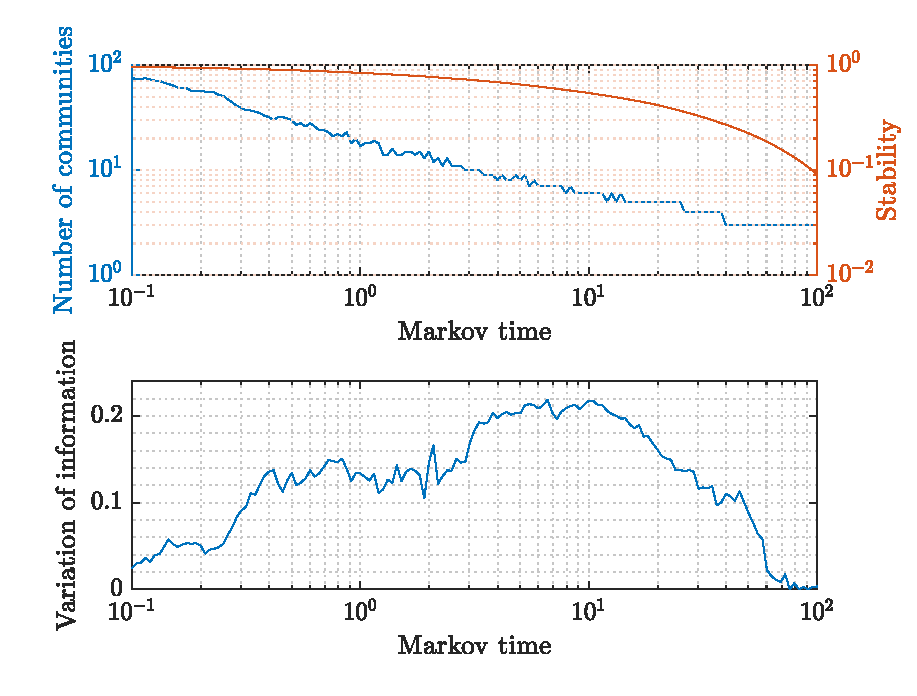
\includegraphics[width = .7\textwidth]{clusters/stab0.eps}
	\caption{Stability, number of communities and variation of information as a function of the Markov time for $T=1$ year.}
	\label{fig:stab0}
\end{figure}

\begin{figure}[H]
	\centering
	\begin{subfigure}[t]{0.49\textwidth}
		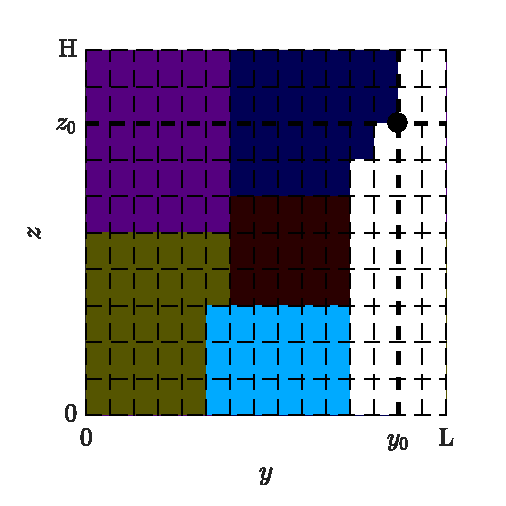
\includegraphics[width=\textwidth]{clusters/cluster0_6_.eps}
		\caption{6 communities.}
		\label{fig:cluster0_6_}
	\end{subfigure}
	\begin{subfigure}[t]{0.49\textwidth}
		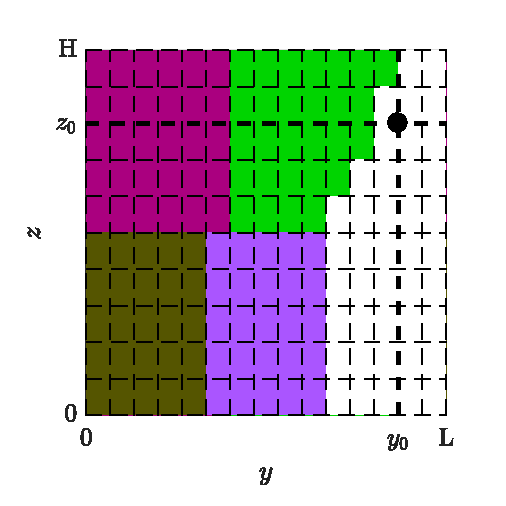
\includegraphics[width=\textwidth]{clusters/cluster0_5_.eps}
		\caption{5 communities.}
		\label{fig:cluster0_5_}
	\end{subfigure}
	\begin{subfigure}[t]{0.49\textwidth}
		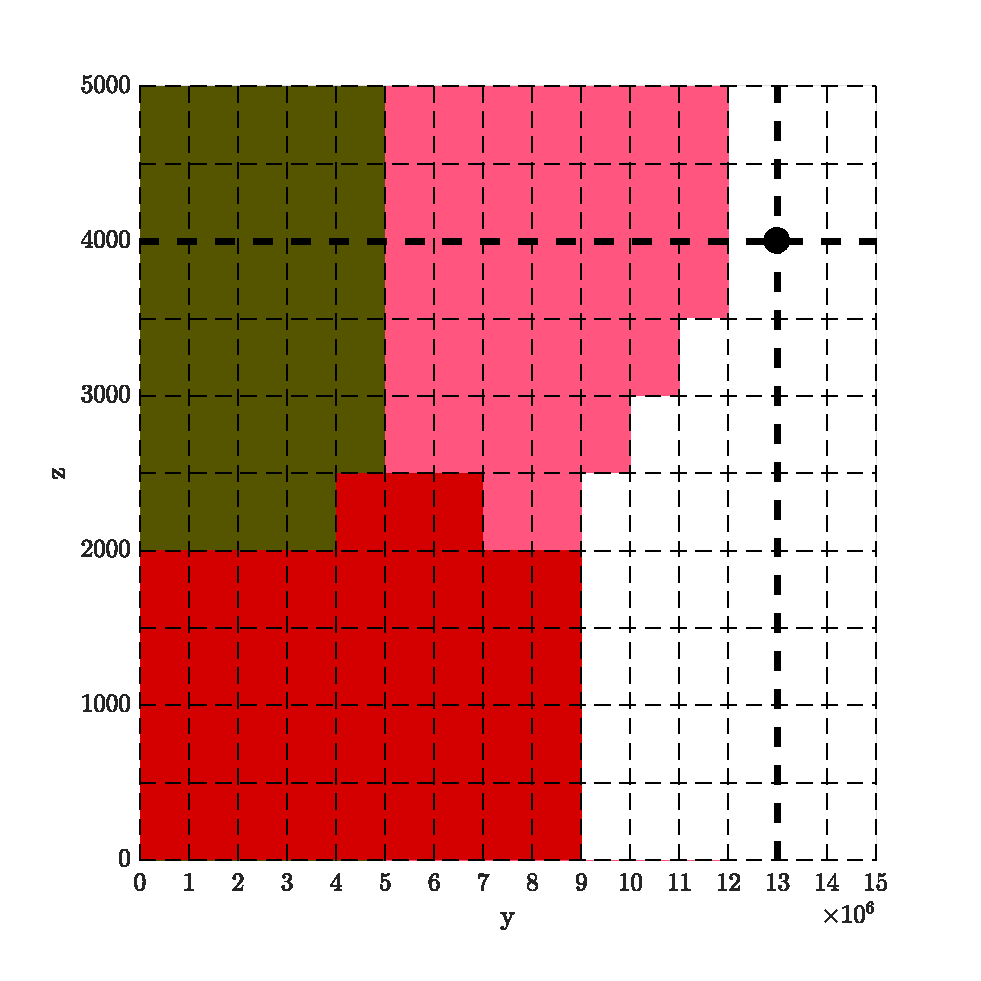
\includegraphics[width=\textwidth]{clusters/cluster0_4_.eps}
		\caption{4 communities.}
		\label{fig:cluster0_4_}
	\end{subfigure}
	\begin{subfigure}[t]{0.49\textwidth}
		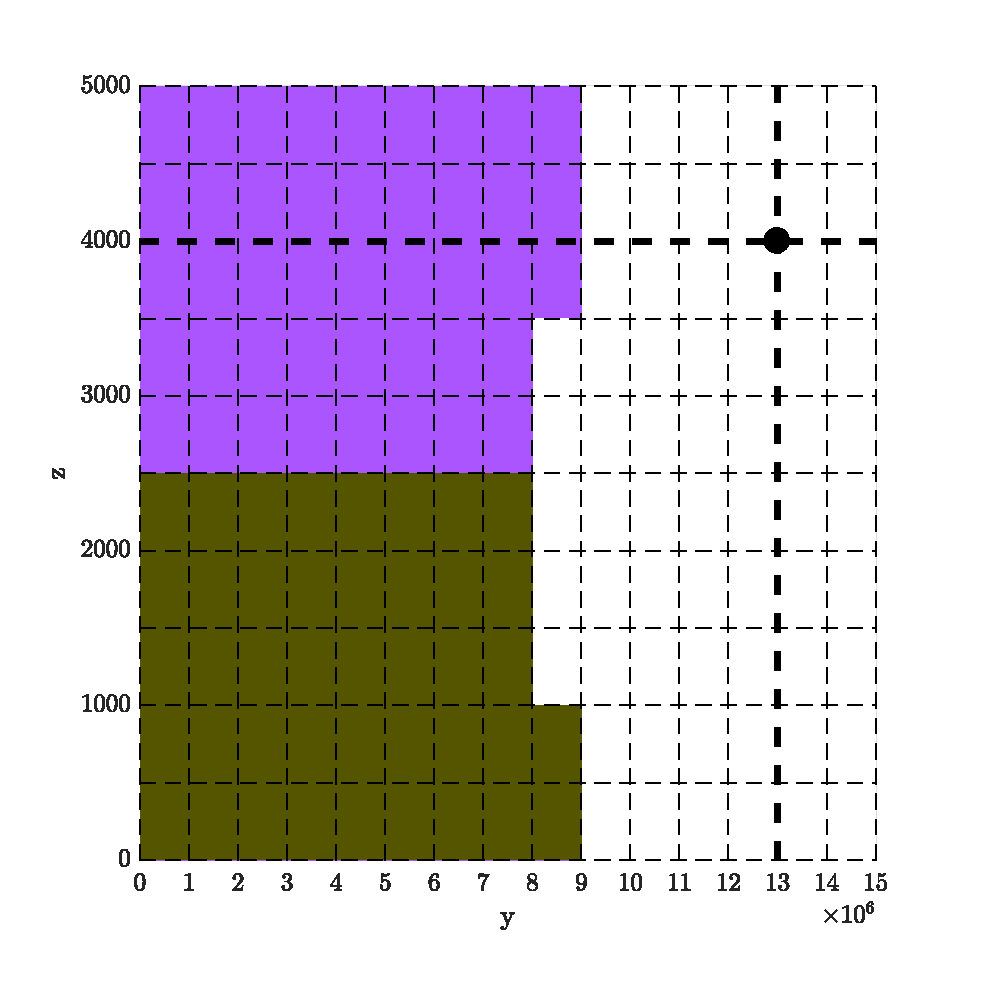
\includegraphics[width=\textwidth]{clusters/cluster0_3_.eps}
		\caption{3 communities.}
		\label{fig:cluster0_3_}
	\end{subfigure}
	\caption{The relevant clusterings detected at different time scales for $T=1$ year.}
	\label{fig:cluster0}
\end{figure}

%------------------ T = 10 -----------------------------%

\begin{figure}[H]
	\centering
	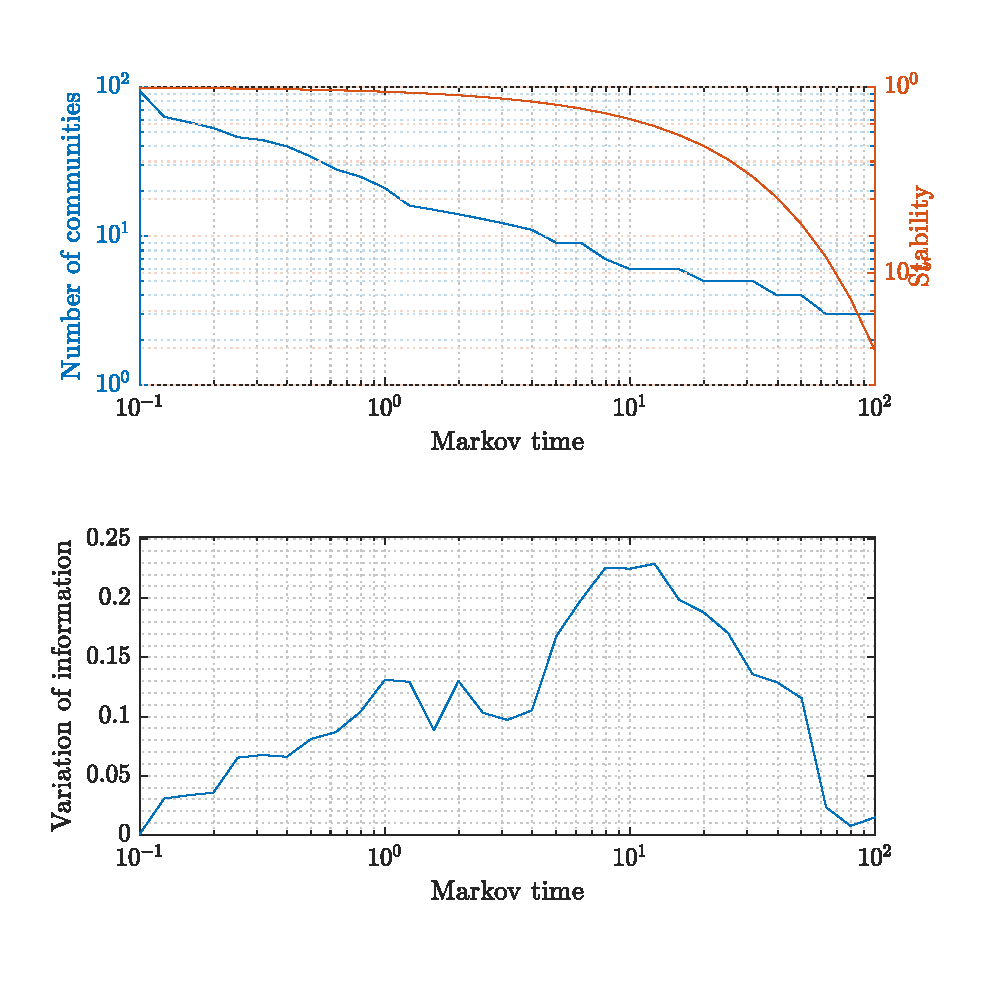
\includegraphics[width = .7\textwidth]{clusters/stab1.eps}
	\caption{Stability, number of communities and variation of information as a function of the Markov time for $T=10$ years.}
	\label{fig:stab1}
\end{figure}

\begin{figure}[H]
	\centering
	\begin{subfigure}[t]{0.49\textwidth}
		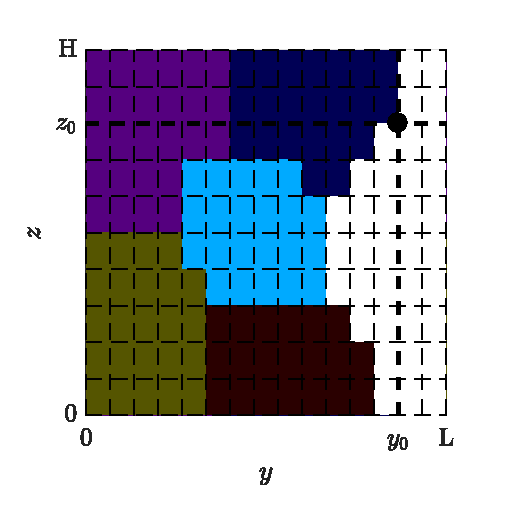
\includegraphics[width=\textwidth]{clusters/cluster1_6_.eps}
		\caption{6 communities.}
		\label{fig:cluster1_6_}
	\end{subfigure}
	\begin{subfigure}[t]{0.49\textwidth}
		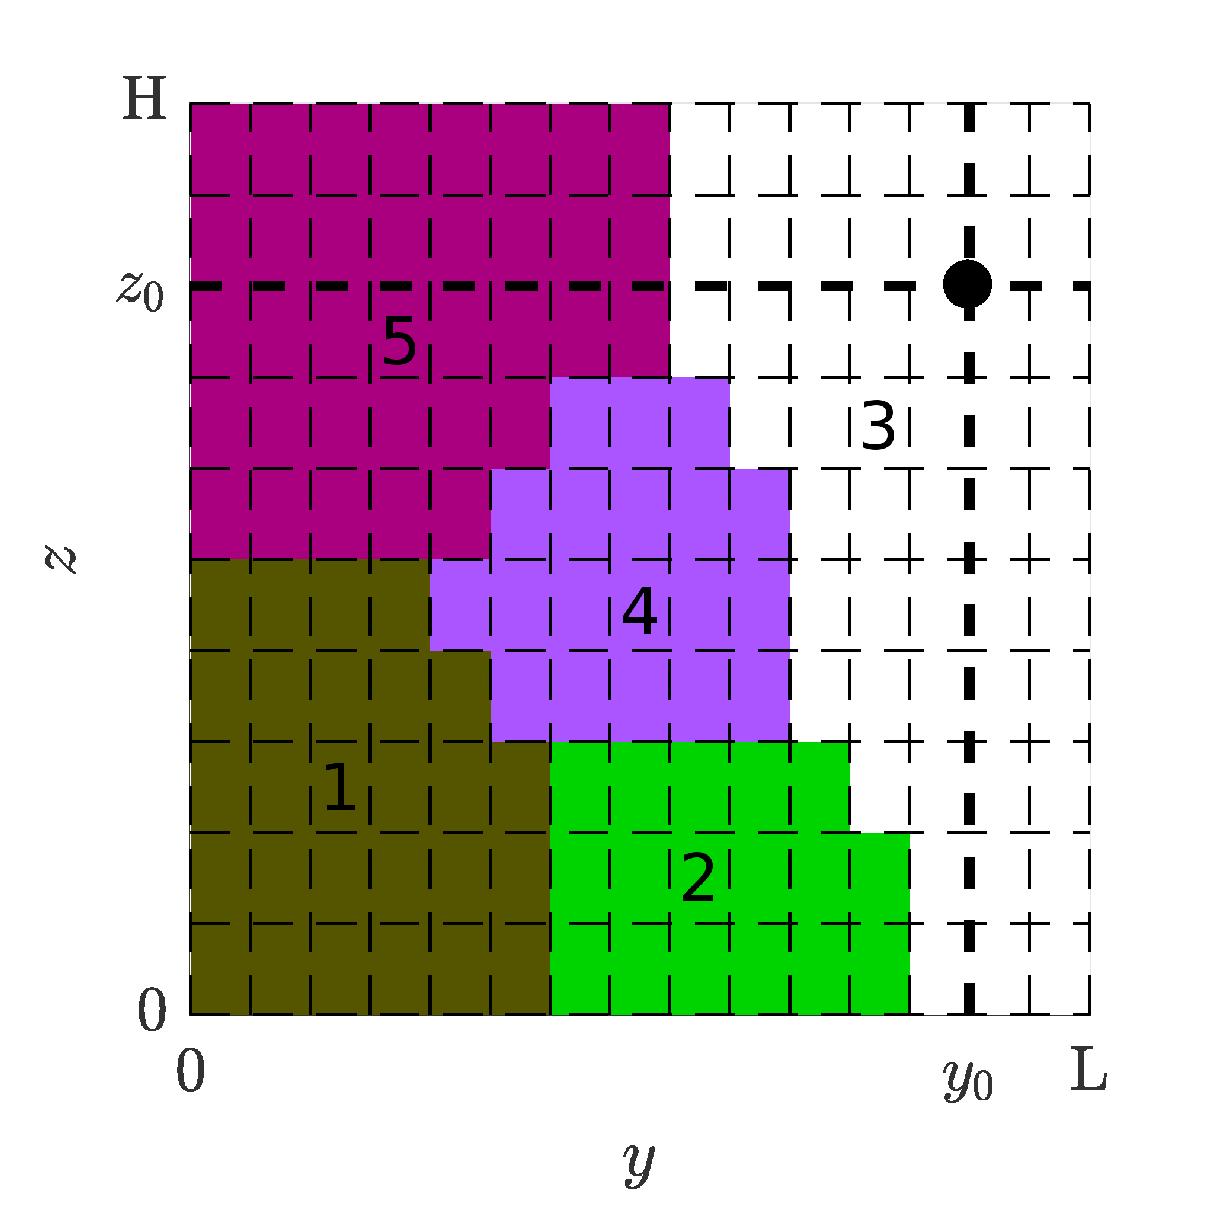
\includegraphics[width=\textwidth]{clusters/cluster1_5_num.eps}
		\caption{5 communities.}
		\label{fig:cluster1_5_}
	\end{subfigure}
	\begin{subfigure}[t]{0.49\textwidth}
		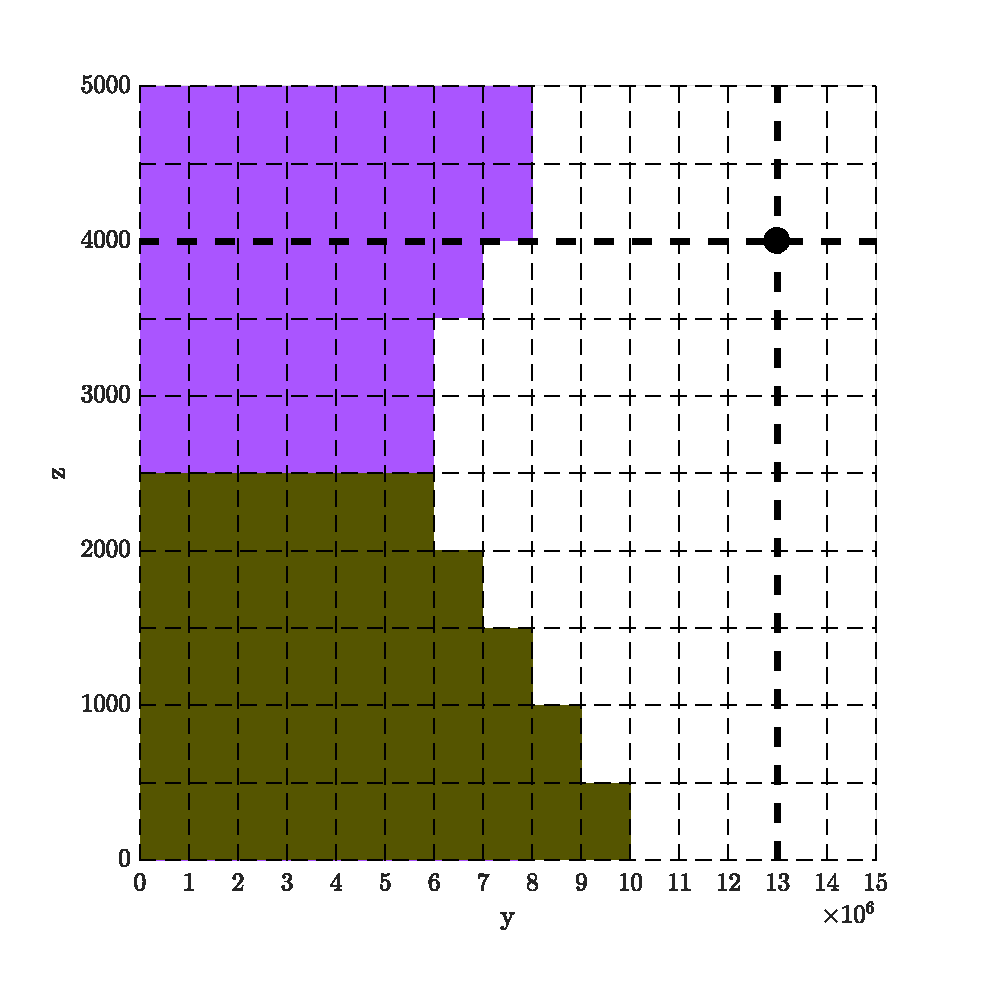
\includegraphics[width=\textwidth]{clusters/cluster1_3_.eps}
		\caption{3 communities.}
		\label{fig:cluster1_3_}
	\end{subfigure}
	\begin{subfigure}[t]{0.49\textwidth}
		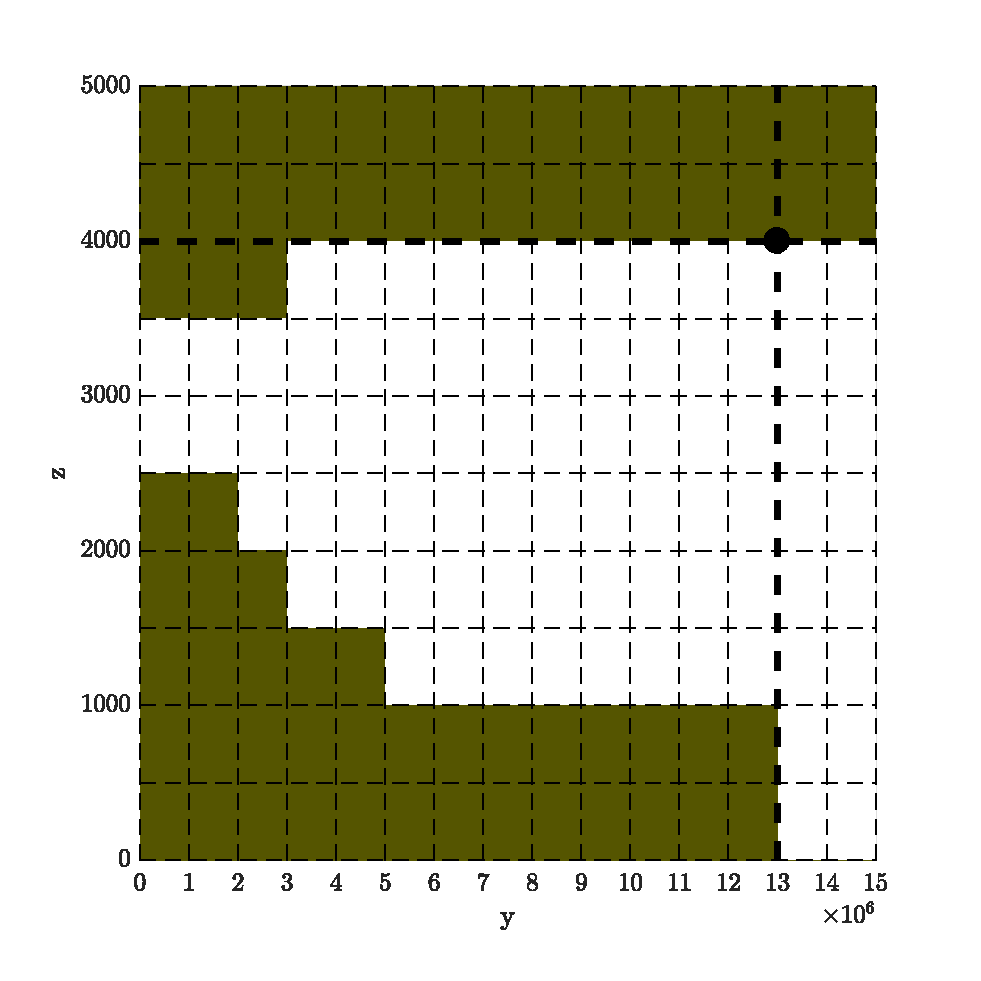
\includegraphics[width=\textwidth]{clusters/cluster1_2_.eps}
		\caption{2 communities detected by the algorithm which should rather be considered as being 3 communities.}
		\label{fig:cluster1_2_}
	\end{subfigure}
	\caption{The relevant clusterings detected at different time scales for $T=10$ years.}
	\label{fig:cluster1}
\end{figure}

%------------------ T = 50 -----------------------------%
\begin{figure}[H]
	\centering
	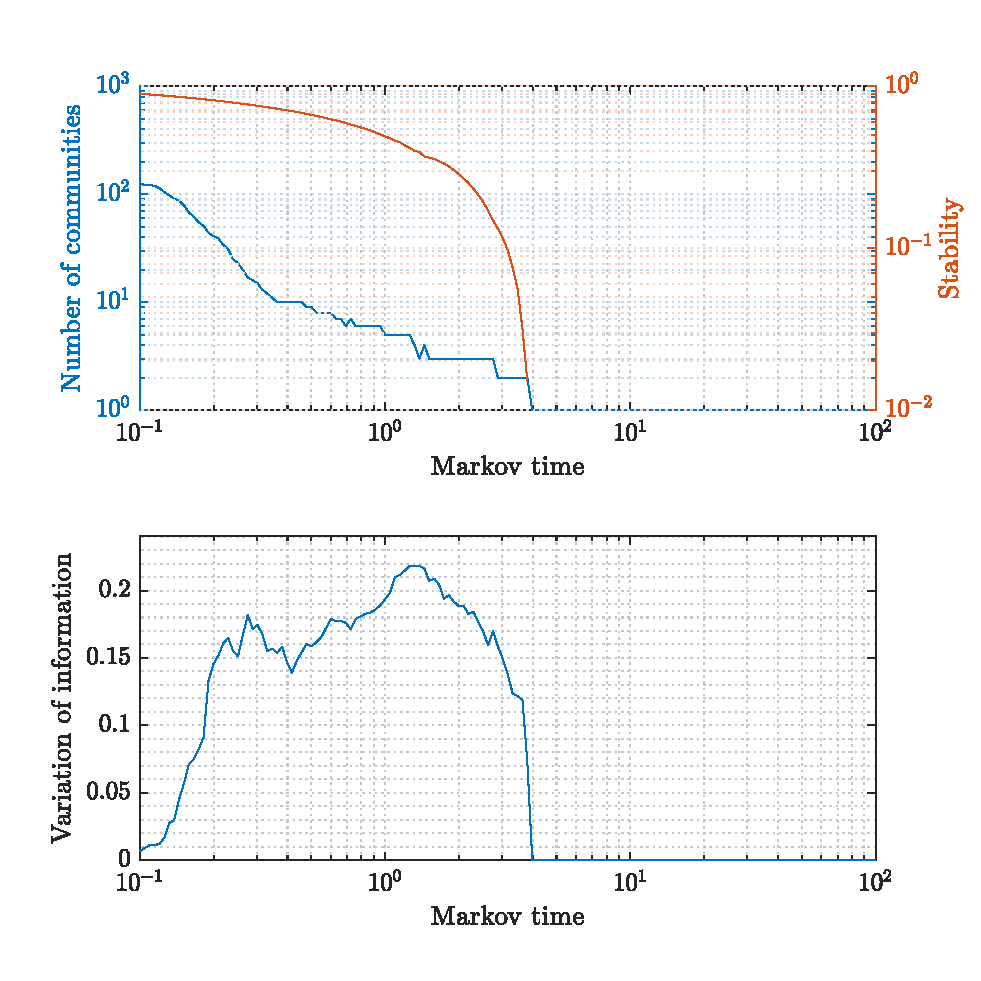
\includegraphics[width = .7\textwidth]{clusters/stab5.eps}
	\caption{Stability, number of communities and variation of information as a function of the Markov time for $T=50$ years.}
	\label{fig:stab5}
\end{figure}

\begin{figure}[H]
	\centering
	\begin{subfigure}[t]{0.49\textwidth}
		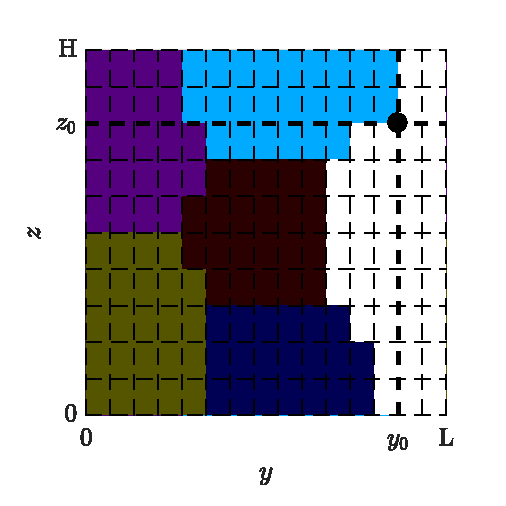
\includegraphics[width=\textwidth]{clusters/cluster5_6_.eps}
		\caption{6 communities.}
		\label{fig:cluster5_6_}
	\end{subfigure}
	\begin{subfigure}[t]{0.49\textwidth}
		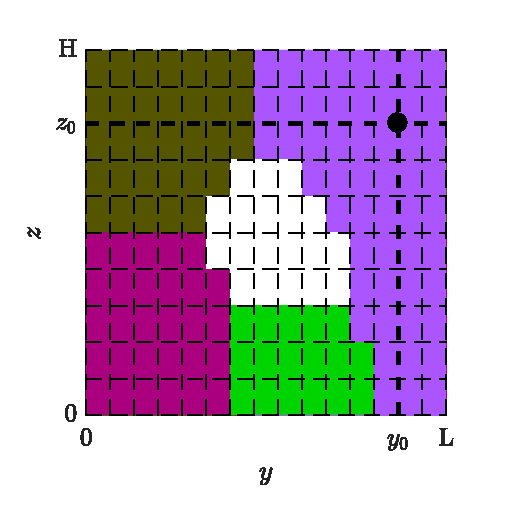
\includegraphics[width=\textwidth]{clusters/cluster5_5_.eps}
		\caption{5 communities.}
		\label{fig:cluster5_5_}
	\end{subfigure}
	\begin{subfigure}[t]{0.49\textwidth}
		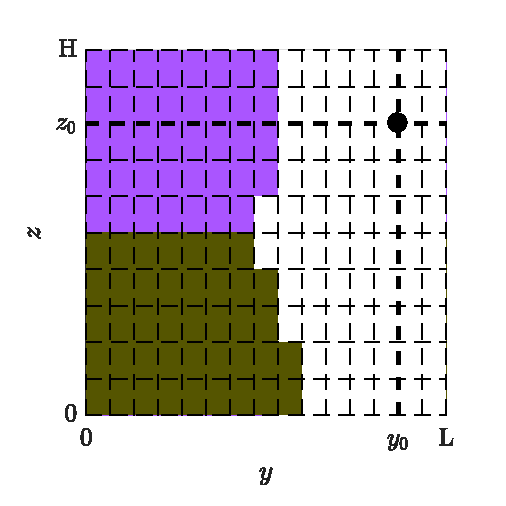
\includegraphics[width=\textwidth]{clusters/cluster5_3_.eps}
		\caption{3 communities.}
		\label{fig:cluster5_3_}
	\end{subfigure}
	\begin{subfigure}[t]{0.49\textwidth}
		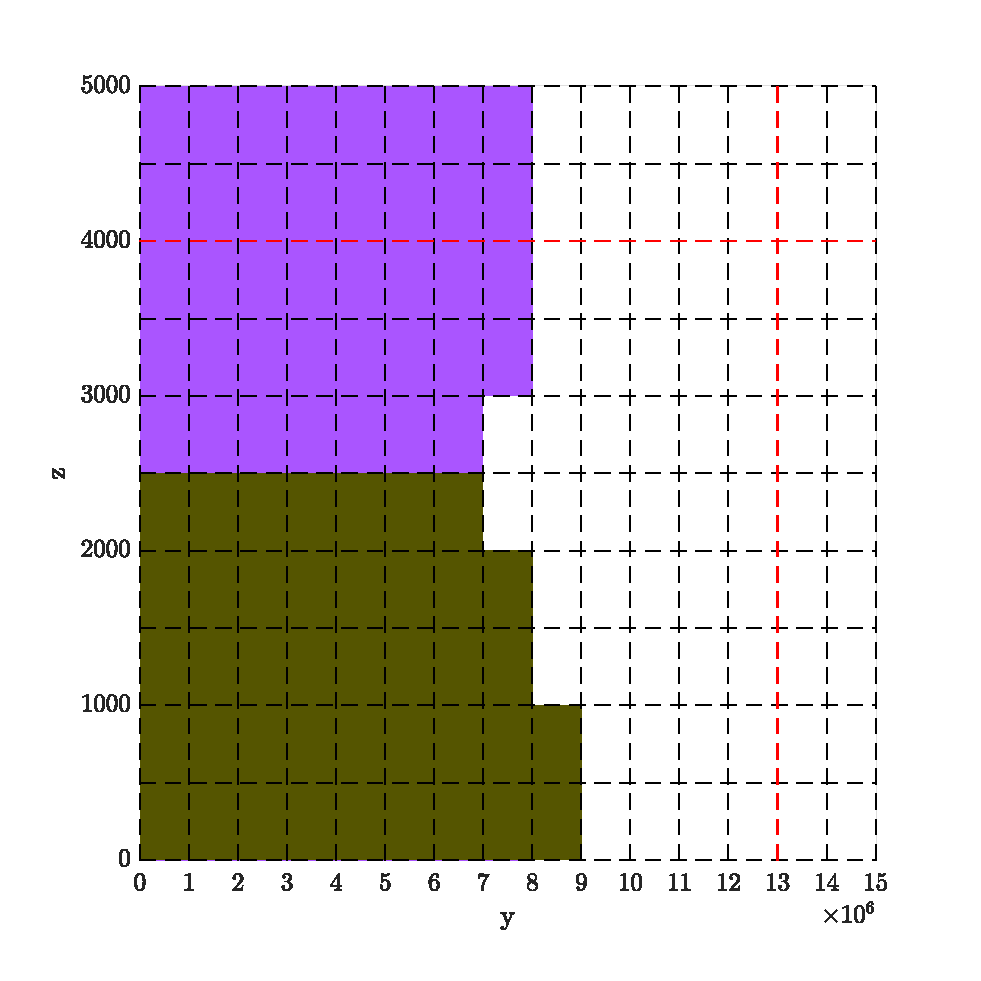
\includegraphics[width=\textwidth]{clusters/cluster5_2_.eps}
		\caption{2 communities.}
		\label{fig:cluster5_2_}
	\end{subfigure}
	\caption{The relevant clusterings detected at different time scales for $T=50$ years.}
	\label{fig:cluster5}
\end{figure}

%------------------ T = 100 ----------------------------%
\begin{figure}[H]
	\centering
	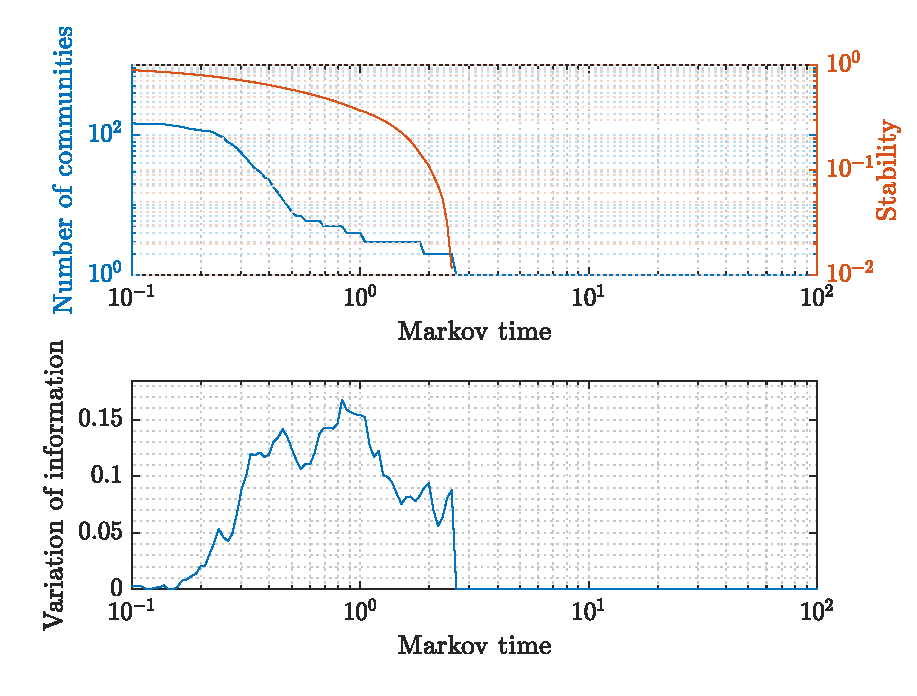
\includegraphics[width = .7\textwidth]{clusters/stab10.eps}
	\caption{Stability, number of communities and variation of information as a function of the Markov time for $T=100$ years.}
	\label{fig:stab10}
\end{figure}

\begin{figure}[H]
	\centering
	\begin{subfigure}[t]{0.49\textwidth}
		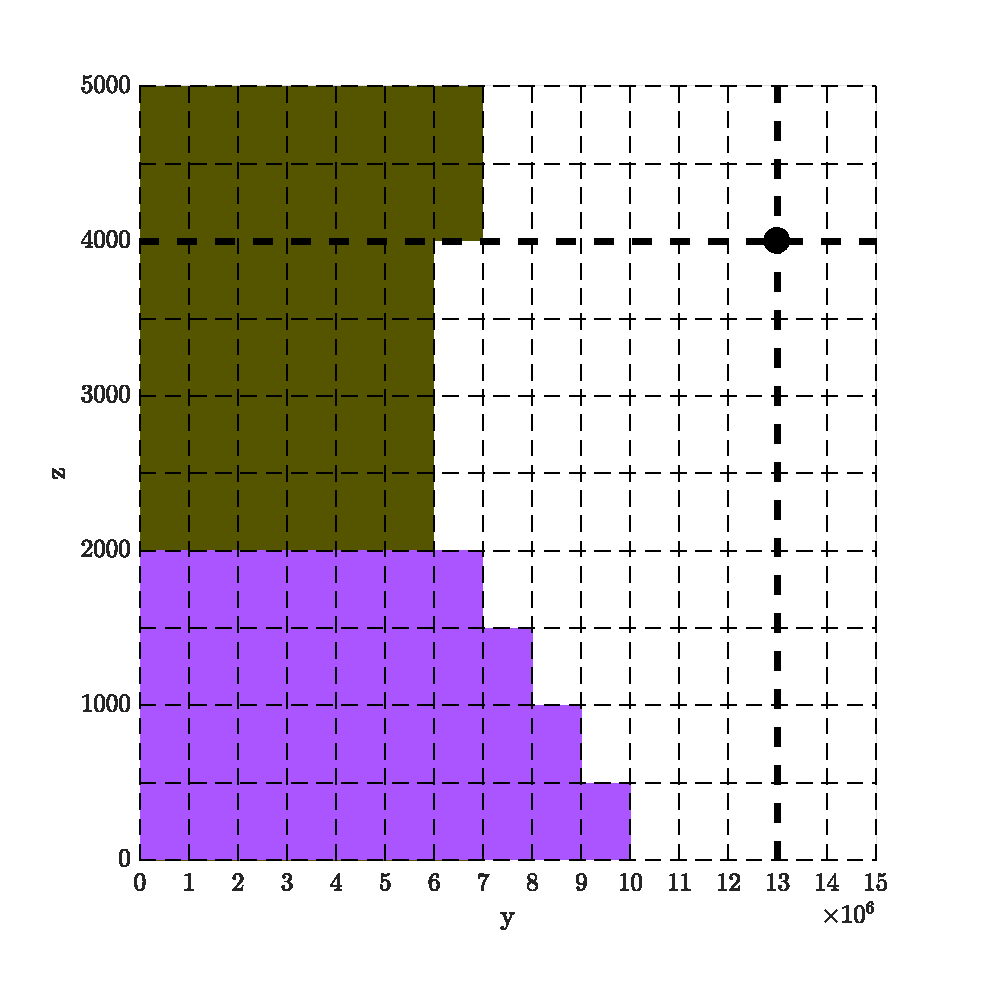
\includegraphics[width=\textwidth]{clusters/cluster10_3_.eps}
		\caption{3 communities.}
		\label{fig:cluster10_3_}
	\end{subfigure}
	\begin{subfigure}[t]{0.49\textwidth}
		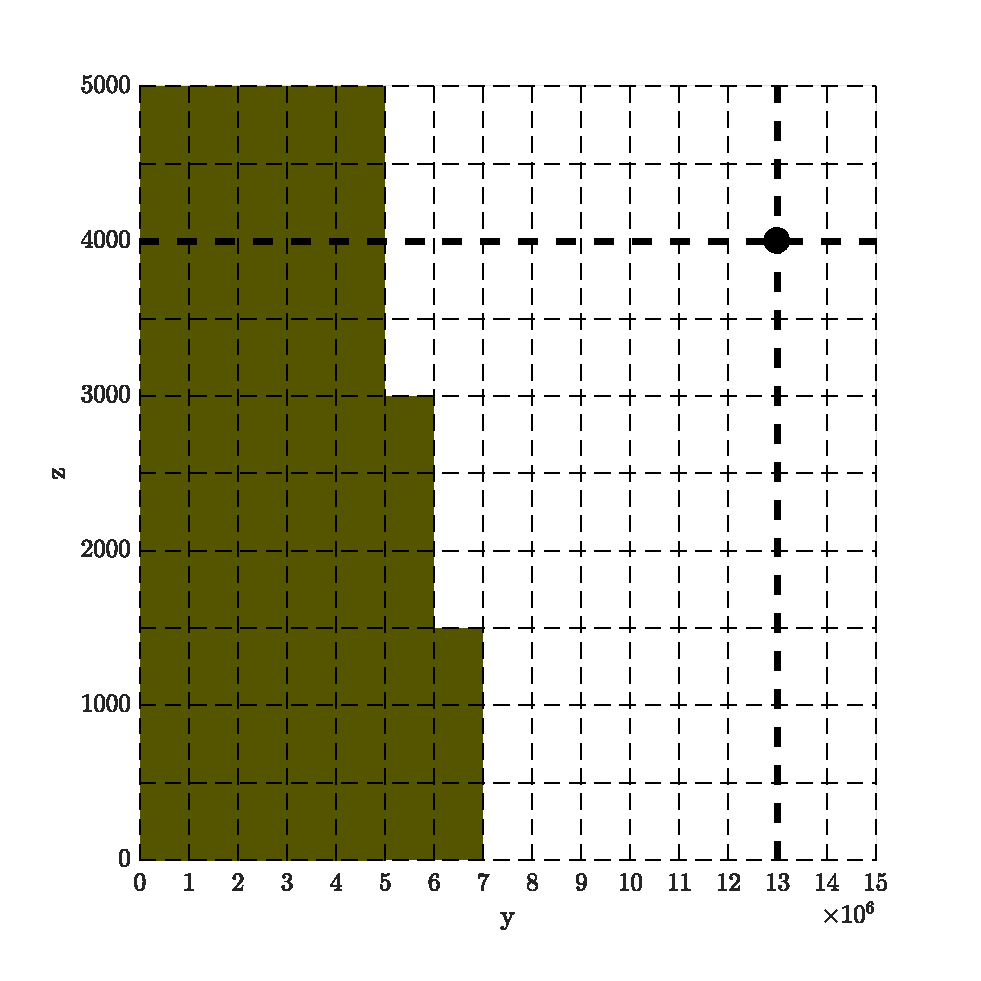
\includegraphics[width=\textwidth]{clusters/cluster10_2_.eps}
		\caption{2 communities.}
		\label{fig:cluster10_2_}
	\end{subfigure}
	\caption{The relevant clusterings detected at different time scales for $T=100$ years.}
	\label{fig:cluster10}
\end{figure}